% ======================================================================
% TRABAJO DE FIN DE GRADO - ETSIIT UNIVERSIDAD DE GRANADA
% Título: Análisis predictivo de fatiga mediante datos biométricos multimodales
% Autor: Emilio Gullón
% Convocatoria: 2025/2026
% ======================================================================

\documentclass[11pt, a4paper, twoside, openright]{report}

% Cargar configuración y paquetes
% ======================================================================
% CONFIGURACIÓN Y PREÁMBULO GLOBAL - MEMORIA TFG ETSIIT - UGR
% ======================================================================

% ---- Codificación e Idioma ----
\usepackage[utf8]{inputenc}
\usepackage[T1]{fontenc}
\usepackage[spanish,es-tabla,es-nodecimaldot]{babel}

% ---- Tipografía y Márgenes ----
\usepackage{lmodern}
\usepackage[a4paper, top=2.5cm, bottom=2.5cm, left=3.0cm, right=2.5cm, headheight=16pt]{geometry}
\renewcommand{\baselinestretch}{1.18} % Interlineado académico profesional

% ---- Matemáticas y Símbolos ----
\usepackage{amsmath, amssymb}
\usepackage{xspace}
\providecommand{\bm}[1]{\mathbf{#1}}

% ---- Tablas y Figuras ----
\usepackage{graphicx}
\usepackage{booktabs}
\usepackage{multirow}
\usepackage{longtable}
\usepackage{tabularx}
\usepackage{array}
\usepackage{float}
\usepackage{caption}
\usepackage{subcaption}

% ---- Encabezados y Pies de Página ----
\usepackage{fancyhdr}
\pagestyle{fancy}
\fancyhf{}
\fancyhead[LE,RO]{\thepage}
\fancyhead[RE]{\small\nouppercase{\leftmark}}
\fancyhead[LO]{\small\nouppercase{\rightmark}}
\renewcommand{\headrulewidth}{0.4pt}
\renewcommand{\footrulewidth}{0pt}

% ---- Colores Corporativos y de Diseño ----
\usepackage{xcolor}
\definecolor{ugrred}{RGB}{198, 12, 48}       % Rojo institucional UGR
\definecolor{etsiitblue}{RGB}{0, 68, 124}     % Azul institucional ETSIIT
\definecolor{darkblue}{RGB}{12, 45, 110}
\definecolor{darkgreen}{RGB}{20, 110, 45}
\definecolor{codebg}{RGB}{248, 249, 250}
\definecolor{codeframe}{RGB}{220, 224, 230}
\definecolor{codekeyword}{RGB}{175, 0, 80}
\definecolor{codestring}{RGB}{20, 130, 40}
\definecolor{codecomment}{RGB}{110, 115, 125}

% ---- Formato de Código Fuente ----
\usepackage{listings}
\lstdefinestyle{pythonstyle}{
    language=Python,
    backgroundcolor=\color{codebg},
    basicstyle=\ttfamily\footnotesize,
    keywordstyle=\color{codekeyword}\bfseries,
    stringstyle=\color{codestring},
    commentstyle=\color{codecomment}\itshape,
    numbers=left,
    numberstyle=\tiny\color{gray},
    stepnumber=1,
    numbersep=8pt,
    frame=single,
    rulecolor=\color{codeframe},
    breaklines=true,
    breakatwhitespace=true,
    showstringspaces=false,
    tabsize=4,
    captionpos=b,
    xleftmargin=1.5em,
    framexleftmargin=1.5em
}
\lstdefinestyle{bashstyle}{
    language=bash,
    backgroundcolor=\color{codebg},
    basicstyle=\ttfamily\footnotesize,
    keywordstyle=\color{codekeyword}\bfseries,
    commentstyle=\color{codecomment}\itshape,
    numbers=none,
    frame=single,
    rulecolor=\color{codeframe},
    breaklines=true,
    showstringspaces=false,
    tabsize=2,
    captionpos=b
}
\lstset{style=pythonstyle}

% ---- Diagramas Vectoriales TikZ ----
\usepackage{tikz}
\usetikzlibrary{shapes.geometric, arrows, positioning, calc, fit, backgrounds, patterns}

% ---- Hipervínculos ----
% Limpiar páginas en blanco creadas por \cleardoublepage sin dependencias externas
\makeatletter
\def\cleardoublepage{\clearpage\if@twoside \ifodd\c@page\else
  \hbox{}\thispagestyle{empty}\newpage\if@twocolumn\hbox{}\newpage\fi\fi\fi}
\makeatother

\usepackage{hyperref}
\hypersetup{
    colorlinks=true,
    linkcolor=etsiitblue,
    citecolor=darkgreen,
    urlcolor=etsiitblue,
    filecolor=etsiitblue,
    pdfauthor={Emilio Gullón},
    pdftitle={Análisis predictivo de fatiga mediante datos biométricos multimodales},
    pdfsubject={Trabajo de Fin de Grado - ETSIIT UGR},
    pdfkeywords={Fatiga Mental, Fatiga Física, FatigueSet, Deep Learning, PyTorch, sLSTM, xLSTM, Foundation Models, MOMENT, Chronos, TimesFM, Optuna, Series Temporales}
}

% ---- Listas e Índices ----
\usepackage{enumitem}
\setlist{itemsep=3pt, topsep=4pt}
\usepackage{tocbibind}

% ---- Comandos y Macros Personalizadas ----
\providecommand{\euro}{€}
\newcommand{\fatigueset}{\textsc{FatigueSet}}
\newcommand{\moment}{\textsc{MOMENT}}
\newcommand{\chronos}{\textsc{Chronos}}
\newcommand{\timesfm}{\textsc{TimesFM}}
\newcommand{\xlstm}{\textsc{xLSTM}}
\newcommand{\slstm}{\textsc{sLSTM}}
\newcommand{\mlstm}{\textsc{mLSTM}}
\newcommand{\patchtst}{\textsc{PatchTST}}
\newcommand{\code}[1]{\texttt{#1}}

% ---- Entornos Teorema/Definición Estándar ----
\newtheorem{definicion}{Definición}[chapter]
\newtheorem{hipotesis}{Hipótesis}[chapter]
\newtheorem{observacion}{Observación}[chapter]


\begin{document}

% ----------------------------------------------------------------------
% PARTE PRELIMINAR (Frontmatter)
% ----------------------------------------------------------------------
\pagenumbering{roman}
% ======================================================================
% PARTE PRELIMINAR (FRONTMATTER) - SEGUIMIENTO DE PLANTILLA UGR ETSIIT
% ======================================================================

% ----------------------------------------------------------------------
% PORTADA PRINCIPAL OFICIAL ETSIIT (Plantilla_TFG_latex/portada/portada.tex)
% ----------------------------------------------------------------------
\begin{titlepage}

\newlength{\centeroffset}
\setlength{\centeroffset}{-0.5\oddsidemargin}
\addtolength{\centeroffset}{0.5\evensidemargin}
\thispagestyle{empty}

\noindent\hspace*{\centeroffset}\begin{minipage}{\textwidth}

\centering

\includegraphics[width=0.9\textwidth]{figures/logo_ugr.jpg}\\[1.4cm]

\textsc{ \Large TRABAJO FIN DE GRADO\\[0.2cm]}
\textsc{ GRADO EN INGENIERÍA INFORMÁTICA}\\[1cm]

% Título Principal Completo
{\Huge\bfseries Análisis predictivo de fatiga mediante datos biométricos multimodales\\
}
\noindent\rule[-1ex]{\textwidth}{3pt}\\[3.5ex]
\end{minipage}

\vspace{2.5cm}
\noindent\hspace*{\centeroffset}\begin{minipage}{\textwidth}
\centering

\textbf{Autor}\\ {Emilio Gullón López}\\[2.5ex]
\textbf{Director}\\
{Diego Jesús García Gil}\\[2cm]

\includegraphics[width=0.3\textwidth]{figures/etsiit_logo.png}\\[0.1cm]
\textsc{Escuela Técnica Superior de Ingenierías Informática y de Telecomunicación}\\
\textsc{---}\\
Granada, Julio de 2026
\end{minipage}
\end{titlepage}

\clearpage

% ----------------------------------------------------------------------
% CRÉDITOS, LICENCIA Y DECLARACIÓN DE USO ÉTICO DE IA
% ----------------------------------------------------------------------
\thispagestyle{empty}
\vspace*{\fill}

\begin{center}
    \textbf{Análisis predictivo de fatiga mediante datos biométricos multimodales}
\end{center}

\vspace{0.5cm}
\noindent\copyright\,2026 por \textbf{Emilio Gullón López}.

\vspace{0.4cm}
\noindent\begin{minipage}{0.15\textwidth}
    
\includegraphics[width=\textwidth]{figures/cc_by_nc_sa.png}
\end{minipage}
\hfill
\begin{minipage}{0.82\textwidth}
\small
Esta memoria de Trabajo de Fin de Grado se distribuye bajo una licencia internacional \textbf{Creative Commons Atribución-NoComercial-CompartirIgual 4.0 Internacional (CC BY-NC-SA 4.0)}. Para consultar los términos legales completos de esta licencia, visite: \url{https://creativecommons.org/licenses/by-nc-sa/4.0/}.

\vspace{0.2cm}
Se autoriza la consulta, copia y redistribución sin fines comerciales, siempre que se reconozca expresamente la autoría original y las obras derivadas se distribuyan bajo la misma licencia. Este documento será depositado en acceso abierto en el repositorio institucional \textbf{Digibug} de la Universidad de Granada (\url{https://digibug.ugr.es}).
\end{minipage}

\vspace{0.8cm}
\noindent\rule{\linewidth}{0.4pt}

\vspace{0.3cm}
\noindent\textbf{Declaración de uso ético de herramientas de Inteligencia Artificial Generativa:}
\begin{small}
En cumplimiento de las directrices del Vicerrectorado de Transformación Digital y del CEPRUD de la Universidad de Granada \cite{ceprud2025ia}, se declara que se han utilizado herramientas de asistencia basada en modelos de lenguaje (LLM) como apoyo para la corrección ortotipográfica y formateo LaTeX. Todo el diseño metodológico, desarrollo de la librería \code{fatigueset-lib}, ejecución experimental y análisis de datos son aportaciones intelectuales originales del autor.
\end{small}

\vspace*{\fill}
\clearpage

% ----------------------------------------------------------------------
% DECLARACIÓN DE AUTORIZACIÓN DE DEPÓSITO EN BIBLIOTECA (PLANTILLA UGR)
% ----------------------------------------------------------------------
\thispagestyle{empty}

\noindent\rule[-1ex]{\textwidth}{2pt}\\[4.5ex]

Yo, \textbf{Emilio Gullón López}, alumno de la titulación Grado en Ingeniería Informática de la \textbf{Escuela Técnica Superior de Ingenierías Informática y de Telecomunicación de la Universidad de Granada}, autorizo la ubicación de la siguiente copia de mi Trabajo Fin de Grado en la biblioteca del centro para que pueda ser consultada por las personas que lo deseen.

\vspace{5cm}

\noindent Fdo: Emilio Gullón López

\vspace{2cm}

\begin{flushright}
Granada, Julio de 2026.
\end{flushright}

\clearpage

% ----------------------------------------------------------------------
% INFORME Y VISTO BUENO DEL DIRECTOR (PLANTILLA UGR)
% ----------------------------------------------------------------------
\thispagestyle{empty}

\noindent\rule[-1ex]{\textwidth}{2pt}\\[4.5ex]

D. \textbf{Diego Jesús García Gil}, Profesor del Departamento de Lenguajes y Sistemas Informáticos de la Universidad de Granada.

\vspace{1.0cm}

\textbf{Informa:}

\vspace{0.8cm}

Que el presente trabajo, titulado \textit{\textbf{Análisis predictivo de fatiga mediante datos biométricos multimodales}}, ha sido realizado bajo su supervisión por \textbf{Emilio Gullón López}, y autoriza la defensa de dicho trabajo ante el tribunal que corresponda.

\vspace{1.0cm}

Y para que conste, expide y firma el presente informe en Granada, Julio de 2026.

\vspace{2cm}

\textbf{El director:}

\vspace{4cm}

\noindent \textbf{Diego Jesús García Gil}

\clearpage

% ----------------------------------------------------------------------
% RESUMEN EN ESPAÑOL (CON FORMATO PLANTILLA UGR)
% ----------------------------------------------------------------------
\thispagestyle{empty}

\begin{center}
{\large\bfseries Análisis predictivo de fatiga mediante datos biométricos multimodales}\\
\end{center}
\begin{center}
Emilio Gullón López (alumno)\\
\end{center}

\vspace{0.5cm}
\noindent{\textbf{Palabras clave}: Predicción de Fatiga, FatigueSet, Señales Fisiológicas Multimodales, Deep Learning, PyTorch, xLSTM, sLSTM, Modelos Fundacionales, MOMENT, Chronos, TimesFM, Optuna, GroupKFold, Series Temporales.}\\

\vspace{0.7cm}
\noindent{\textbf{Resumen}}\\

La fatiga humana es un fenómeno psicofisiológico complejo que deteriora de forma crítica el rendimiento cognitivo, la coordinación motora y la toma de decisiones, constituyendo una de las principales causas de accidentes laborales, siniestros viales y patologías crónicas por estrés. La monitorización objetiva y no invasiva de la fatiga en entornos cotidianos representa un desafío abierto en la intersección entre computación ubicua, procesamiento de bioseñales y aprendizaje profundo.

Este Trabajo de Fin de Grado aborda el modelado cuantitativo y la predicción simultánea de fatiga física y mental a partir de señales fisiológicas multimodales registradas mediante dispositivos vestibles. Se utiliza el dataset de referencia internacional \fatigueset{}, que recopila registros de 12 participantes mediante cuatro dispositivos comerciales (Empatica E4, Zephyr BioHarness 3.0, Muse S y Nokia eSense), totalizando 23 canales fisiológicos heterogéneos (ritmo cardíaco, HRV, actividad electrodérmica EDA, EEG en cuatro bandas espectrales, frecuencia respiratoria y acelerometría triaxial).

En el plano metodológico e ingenieril, se ha desarrollado la librería modular en Python \code{fatigueset-lib}, que desacopla la carga de datos, el procesamiento temporal de señales (filtrado, segmentación en ventanas y extracción de características estadísticas y espectrales), la factoría de modelos de redes neuronales en PyTorch, la optimización bayesiana de hiperparámetros mediante el algoritmo TPE con Optuna, y la evaluación reproducible mediante validación cruzada estratificada por participante (\textit{GroupKFold}).

Se ha llevado a cabo un estudio comparativo exhaustivo que abarca cuatro paradigmas de modelado:
\begin{enumerate}
    \item \textbf{Modelos Clásicos de Machine Learning:} Baselines tabulares (Random Forest, KNN, Árboles de Decisión, Ridge y SVR).
    \item \textbf{Redes Neuronales Profundas Clásicas y Recurrentes:} RNN estándar, LSTM y GRU.
    \item \textbf{Arquitecturas Avanzadas de Series Temporales:} TCN, modelos híbridos CNN-LSTM, Transformers, \patchtst{} y la reciente arquitectura recurrente extendida \xlstm{} (implementando la variante estabilizada \slstm{}).
    \item \textbf{Modelos Fundacionales de Series Temporales:} Evaluación en régimen \textit{zero-shot} y \textit{fine-tuning} de arquitecturas preentrenadas: \moment{}, \chronos{} y \timesfm{} 2.5, desplegados en un clúster universitario GPU con SLURM.
\end{enumerate}

Los resultados experimentales demuestran que las arquitecturas recurrentes optimizadas con Optuna (Custom GRU con $\text{MAE}=16.99$, Custom \xlstm{} con $\text{MAE}=17.33$ y Custom LSTM con $\text{MAE}=17.50$) ofrecen el equilibrio óptimo entre precisión predictiva, estabilidad y eficiencia computacional. Asimismo, los modelos fundacionales como Chronos-T5 demuestran una prometedora capacidad \textit{zero-shot} ($\text{MAE}=14.11$ en fatiga física), aunque con un coste computacional significativamente superior. El trabajo concluye con el análisis del impacto ético, la privacidad de datos biométricos y la alineación con los Objetivos de Desarrollo Sostenible (ODS 3, 8 y 9).

\clearpage

% ----------------------------------------------------------------------
% ABSTRACT IN ENGLISH (CON FORMATO PLANTILLA UGR)
% ----------------------------------------------------------------------
\thispagestyle{empty}

\begin{center}
{\large\bfseries Predictive Fatigue Analysis Using Multimodal Biometric Data}\\
\end{center}
\begin{center}
Emilio Gullón López (student)\\
\end{center}

\vspace{0.5cm}
\noindent{\textbf{Keywords}: Fatigue Prediction, FatigueSet, Multimodal Physiological Signals, Deep Learning, PyTorch, xLSTM, sLSTM, Foundation Models, MOMENT, Chronos, TimesFM, Optuna, GroupKFold, Time Series.}\\

\vspace{0.7cm}
\noindent{\textbf{Abstract}}\\

Human fatigue is a complex psychophysiological phenomenon that critically impairs cognitive performance, motor coordination and decision-making, constituting one of the leading causes of occupational accidents, road incidents and chronic stress-related pathologies. Objective, non-invasive fatigue monitoring in real-world settings remains an open challenge at the intersection of ubiquitous computing, biosignal processing and deep learning.

This Bachelor's Thesis addresses the quantitative modelling and simultaneous prediction of physical fatigue and mental fatigue from multimodal physiological signals recorded by wearable devices. To this end, the international benchmark dataset \fatigueset{} is employed, which collects continuous physiological recordings from 12 participants across cognitive and physical sessions using four commercial devices (Empatica E4, Zephyr BioHarness 3.0, Muse S and Nokia eSense), comprising 23 heterogeneous physiological channels (heart rate, heart rate variability HRV, electrodermal activity EDA, electroencephalography EEG in four spectral bands, respiratory rate and triaxial accelerometry).

From a methodological and software engineering perspective, the modular library \code{fatigue\-set-\-lib} has been designed and implemented in Python, decoupling data loading, temporal signal processing (filtering, windowing and extraction of statistical and spectral features), a PyTorch neural network model factory, Bayesian hyperparameter optimisation via the TPE (\textit{Tree-structured Parzen Estimator}) algorithm with Optuna, and reproducible evaluation through participant-stratified cross-validation (\textit{GroupKFold}) to ensure the complete absence of data leakage.

A comprehensive comparative study has been conducted spanning four modelling paradigms:
\begin{enumerate}
    \item \textbf{Classical Machine Learning Models:} Tabular baselines (Random Forest, KNN, Decision Trees, Ridge and SVR).
    \item \textbf{Classical and Recurrent Deep Neural Networks:} Standard RNN, LSTM and GRU.
    \item \textbf{Advanced Time Series Architectures:} Dilated causal temporal convolutions (TCN), spatio-temporal hybrid models (CNN-LSTM), time series Transformers, patch-based models (\patchtst{}) and the recent extended recurrent architecture \xlstm{} (implementing the stabilised variant \slstm{}).
    \item \textbf{Time Series Foundation Models:} Zero-shot and fine-tuning evaluation of large-scale pretrained architectures: \moment{}, \chronos{} and \timesfm{} 2.5, deployed on a university GPU cluster managed by SLURM.
\end{enumerate}

Experimental results demonstrate that Optuna-optimised recurrent architectures (Custom GRU with $\text{MAE}=16.99$, Custom \xlstm{} with $\text{MAE}=17.33$ and Custom LSTM with $\text{MAE}=17.50$) achieve the optimal balance between predictive accuracy, stability and computational efficiency. Furthermore, foundation models such as Chronos-T5 exhibit promising zero-shot inference capability ($\text{MAE}=14.11$ on physical fatigue), albeit with significantly higher computational cost. The work concludes with an analysis of ethical impact, biometric data privacy and alignment with the Sustainable Development Goals (SDGs 3, 8 and 9).

\cleardoublepage

% ----------------------------------------------------------------------
% AGRADECIMIENTOS
% ----------------------------------------------------------------------
\chapter*{Agradecimientos}
\addcontentsline{toc}{chapter}{Agradecimientos}

A mi familia, por su apoyo incondicional y paciencia infinita a lo largo de todos estos años de formación académica. Su aliento en los momentos de mayor fatiga ha sido el verdadero motor que ha hecho posible la culminación de este grado.

A la persona que ha tutorizado este Trabajo de Fin de Grado, por su guía experta, rigor científico, disponibilidad constante y certeras orientaciones tanto en la formulación del problema como en la revisión de los resultados experimentales.

A mis compañeros y amigos de la Escuela Técnica Superior de Ingenierías Informática y de Telecomunicación (ETSIIT), con quienes he compartido interminables sesiones de estudio, proyectos y debates que han enriquecido mi crecimiento personal y profesional como ingeniero informático.

Al profesorado de la Universidad de Granada, por transmitir con vocación los fundamentos científicos y técnicos de la computación y la ciencia de datos. Asimismo, agradezco al Centro de Servicios de Informática y Redes de Comunicación (CSIRC) por proveer la infraestructura de computación de altas prestaciones en el clúster GPU universitario.

\vspace{1cm}
\begin{flushright}
    \emph{Emilio Gullón López}\\
    \emph{Granada, Julio de 2026}
\end{flushright}

\cleardoublepage

% ----------------------------------------------------------------------
% ÍNDICES GENERALES
% ----------------------------------------------------------------------
\tableofcontents
\cleardoublepage

\listoffigures
\cleardoublepage

\listoftables
\cleardoublepage


% ----------------------------------------------------------------------
% CUERPO PRINCIPAL DE LA MEMORIA (Mainmatter)
% ----------------------------------------------------------------------
\cleardoublepage
\pagenumbering{arabic}

% Capítulo 1: Introducción
% ======================================================================
% CAPÍTULO 1: INTRODUCCIÓN
% ======================================================================

\chapter{Introducción}
\label{cap:introduccion}

\section{Contexto y Antecedentes}
\label{sec:intro_contexto}

Cualquier persona ha experimentado en algún momento de su vida la sensación de agotamiento tras una larga jornada de trabajo o esfuerzo prolongado. Sin embargo, en entornos profesionales de alta responsabilidad ---como la conducción de vehículos de transporte, la intervención quirúrgica en hospitales, el control del tráfico aéreo o la operación de maquinaria industrial pesada--- la fatiga no es un simple malestar pasajero: representa un deterioro inadvertido pero crítico de la capacidad de reacción y juicio que puede desembocar en accidentes graves o pérdidas humanas. En la era de la computación ubicua y los dispositivos inteligentes de uso cotidiano, surge una pregunta científica e ingenieril apasionante: ¿es posible detectar y predecir de forma objetiva, automática y no invasiva este estado de agotamiento fisiológico a partir de señales biométricas registradas por sensores vestibles antes de que se produzca una falla de seguridad?

Desde una perspectiva psicofisiológica formal, la fatiga no constituye un estado unívoco ni estático, sino un proceso dinámico de degradación progresiva de la capacidad funcional, derivado de la actividad sostenida en el tiempo, la privación de descanso o la sobrecarga psicofísica \cite{enoka2008muscle, grandjean1979fatigue}. En el ámbito de la ingeniería informática y las ciencias biomédicas, resulta indispensable delimitar con precisión la terminología empleada, distinguiendo formalmente entre cuatro conceptos estrechamente vinculados pero metodológicamente diferenciados:
\begin{itemize}
    \item \textbf{Fatiga Física (o Periférica/Muscular):} Se define como la reducción transitoria y reversible de la capacidad máxima de generación de fuerza o potencia mecánica de los grupos musculares tras un esfuerzo contráctil sostenido o repetitivo \cite{enoka2008muscle}. A nivel metabólico y sistémico, involucra el agotamiento de sustratos energéticos, la acumulación de metabolitos (como el lactato y protones $H^+$) y alteraciones en el acoplamiento excitación-contracción en las fibras musculares.
    \item \textbf{Fatiga Mental (o Central/Cognitiva):} Es un estado psicofisiológico inducido por la ejecución prolongada de tareas cognitivas exigentes, caracterizado por una sensación subjetiva de cansancio, disminución del estado de alerta, ralentización en los tiempos de reacción y un deterioro sensible en las funciones ejecutivas, tales como la memoria de trabajo, la atención sostenida y la flexibilidad cognitiva \cite{boksem2005effects}.
    \item \textbf{Somnolencia (\textit{Sleepiness}):} Hace referencia a la propensión, presión homeostática o necesidad biológica inminente hacia el sueño \cite{akerstedt1990subjective, hoddes1973quantification}, la cual, aunque interactúa con la fatiga mental, obedece a ritmos circadianos e historia previa de vigilia.
    \item \textbf{Fatigabilidad (\textit{Fatigability}):} Describe la tasa o velocidad a la que un individuo particular experimenta fatiga ante una carga de trabajo estandarizada, reflejando diferencias individuales intrínsecas en la tolerancia al esfuerzo \cite{kalanadhabhatta2021fatigueset}.
\end{itemize}

Históricamente, la cuantificación de la fatiga se ha sustentado de manera predominante en instrumentos de autoevaluación subjetiva mediante cuestionarios psicométricos estandarizados, tales como la Escala de Somnolencia de Stanford (SSS) \cite{hoddes1973quantification}, la Escala Visual Analógica (VAS), la escala de esfuerzo percibido de Borg o el índice NASA-TLX. Si bien estas escalas proporcionan una ventana directa a la percepción del usuario, presentan severas limitaciones metodológicas: adolecen de sesgos de memoria, susceptibilidad al estado anímico, baja resolución temporal y la necesidad imperativa de interrumpir la actividad del sujeto para su cumplimentación, lo que invalida su aplicabilidad en escenarios de monitorización continua en tiempo real. Para superar estas barreras mediante monitorización biomédica continua, en este trabajo se formula un estudio exhaustivo sustentado en una taxonomía integral de paradigmas computacionales (esquematizada en la Figura~\ref{fig:intro_taxonomia}).

\begin{figure}[H]
    \centering
    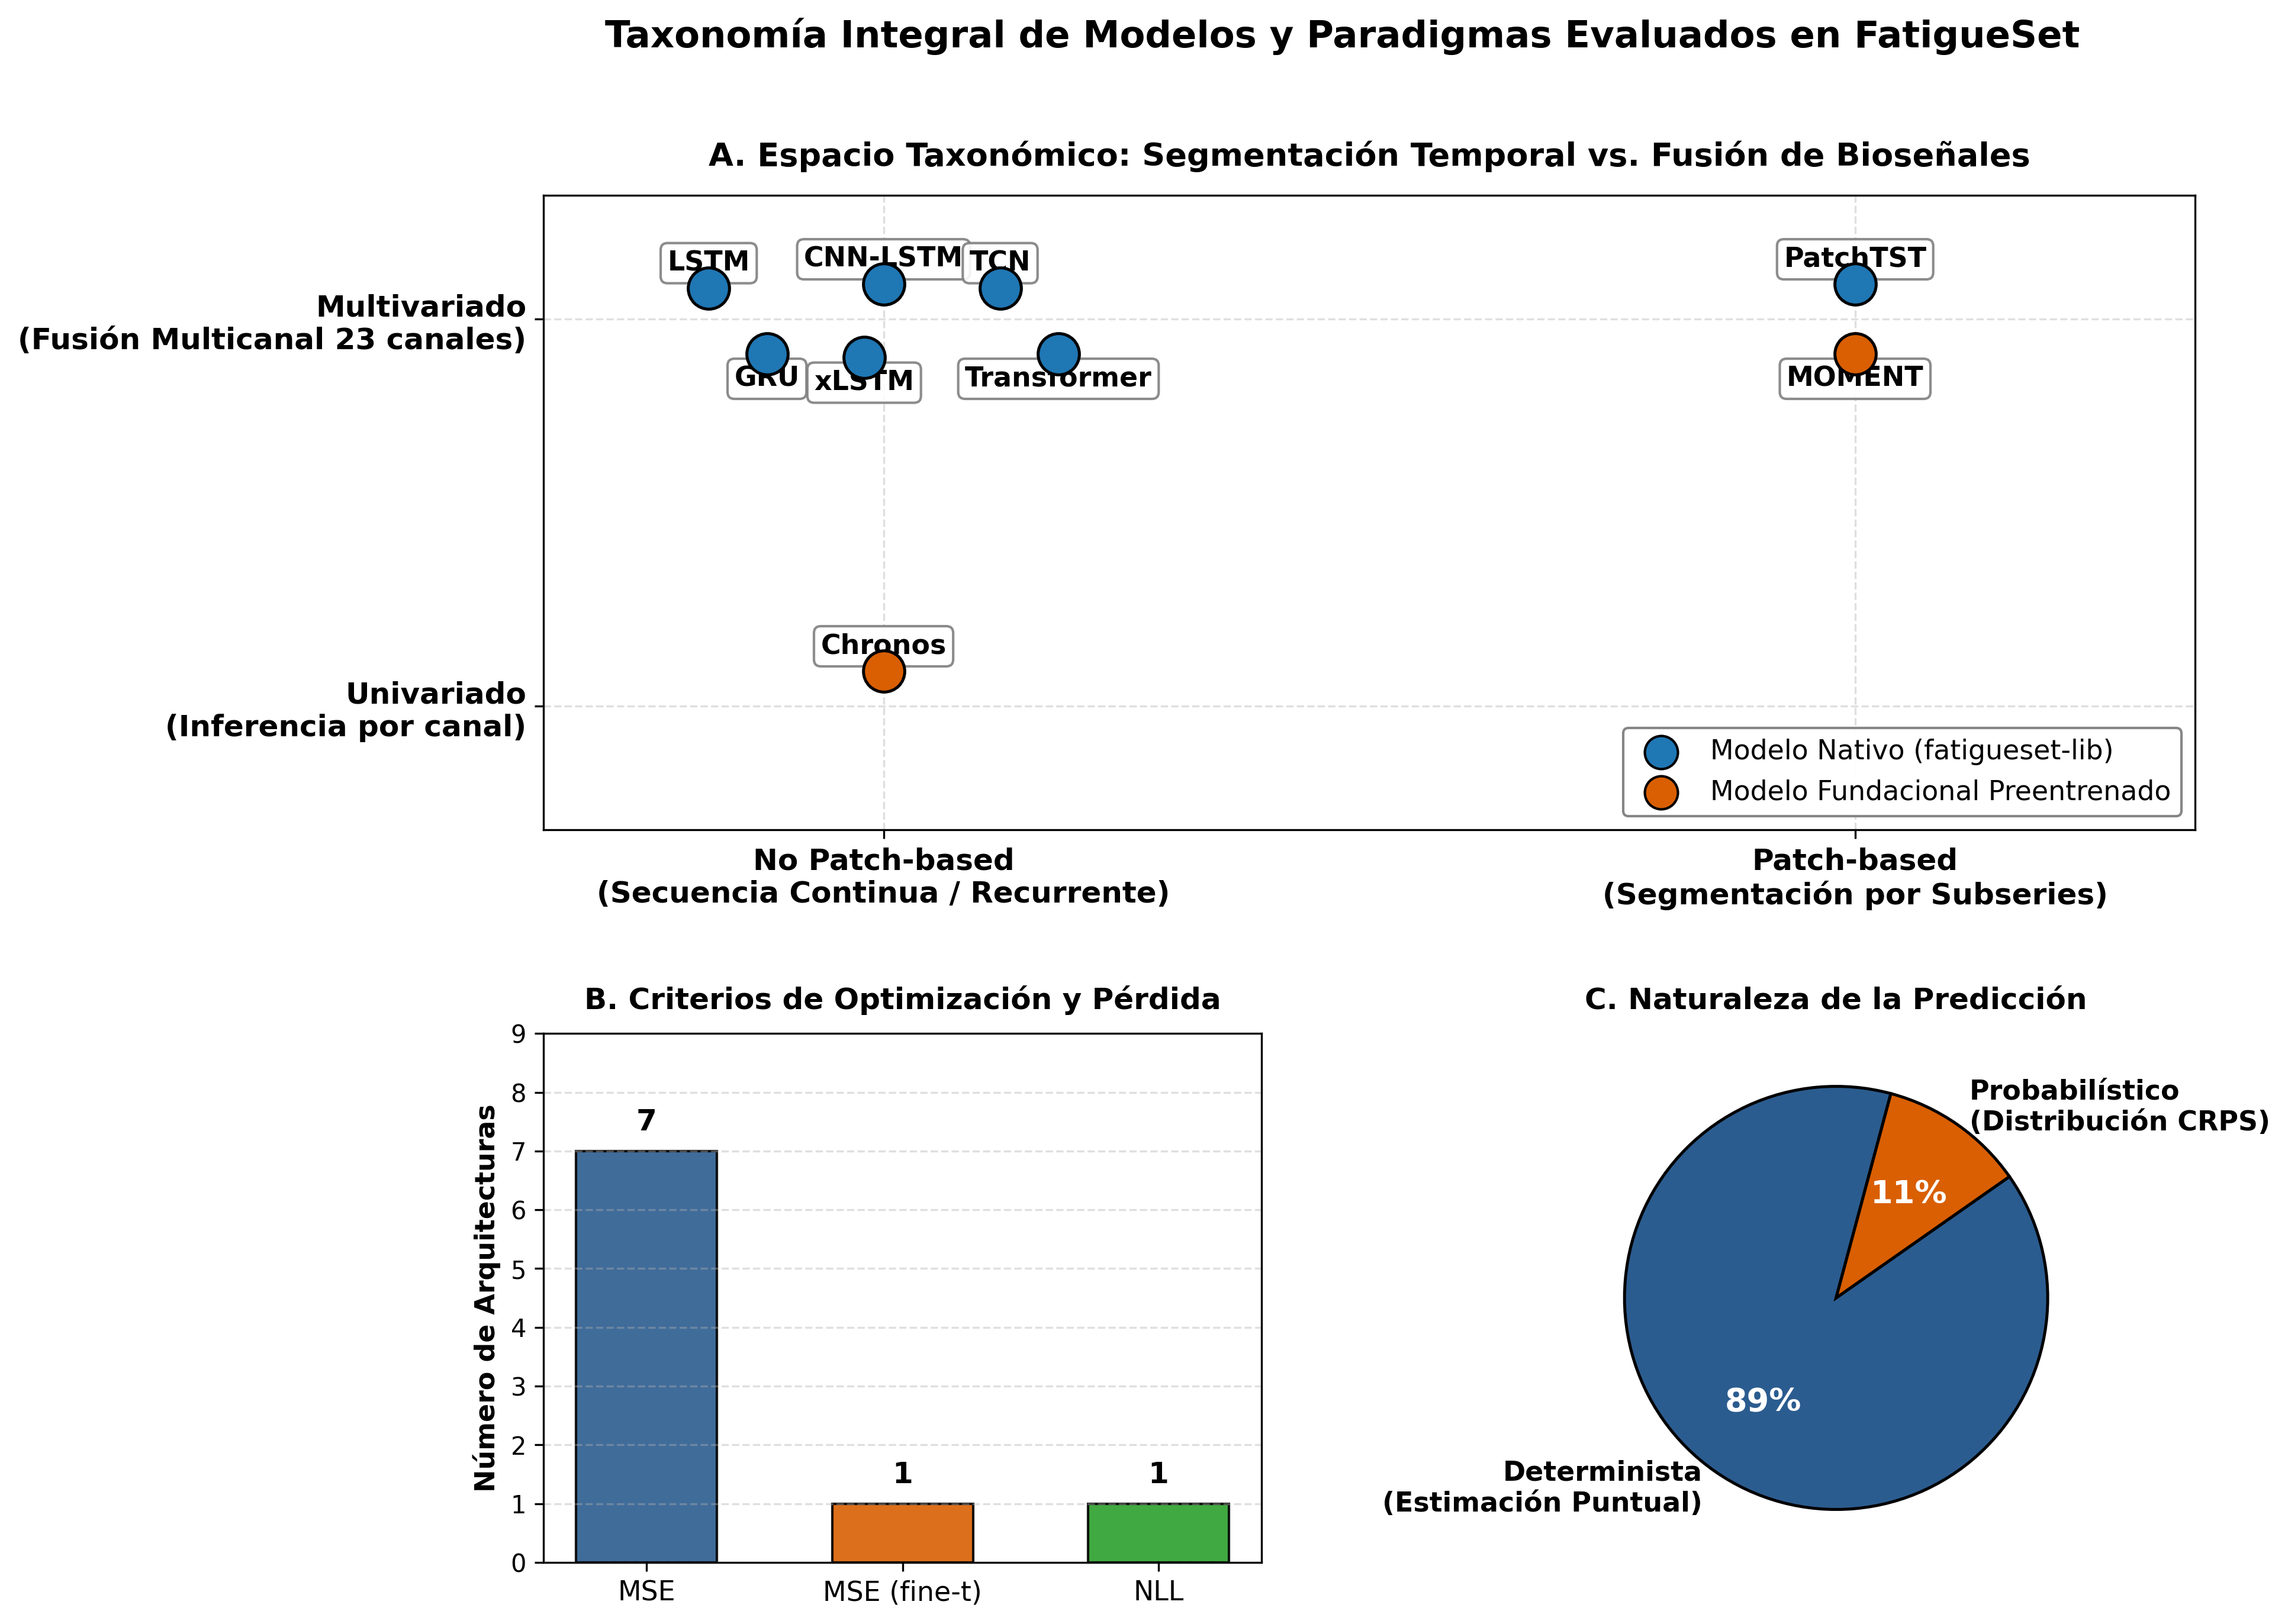
\includegraphics[width=0.86\textwidth]{figures/taxonomia_modelos_tfg.png}
    \caption{Taxonomía integral de modelos y paradigmas evaluados en este Trabajo de Fin de Grado: (A) espacio de segmentación temporal y fusión multicanal de bioseñales, (B) funciones de pérdida y criterios de optimización, y (C) naturaleza determinista frente a probabilística de la predicción. (Fuente: Elaboración propia).}
    \label{fig:intro_taxonomia}
\end{figure}

En la última década, la convergencia entre la microelectrónica de bajo consumo, la computación ubicua (\textit{ubiquitous computing}) y los sensores biomédicos no invasivos ha impulsado la proliferación de dispositivos vestibles (\textit{wearables}) de alta precisión \cite{kalanadhabhatta2022fatigueset}. Dispositivos comerciales como pulseras de fotopletismografía y conductancia cutánea (Empatica E4), bandas torácicas con electrocardiografía y monitorización respiratoria (Zephyr BioHarness 3.0), diademas de electroencefalografía (Muse S) y sensores intrauriculares (Nokia eSense) permiten registrar de forma ininterrumpida bioseñales complejas como:
\begin{enumerate}
    \item \textbf{Variabilidad de la Frecuencia Cardíaca (HRV):} Reflejo de la modulación autonómica simpática y parasimpática en el nódulo sinoauricular \cite{taskforce1996heart}.
    \item \textbf{Actividad Electrodérmica (EDA):} Indicador directo de la activación simpática periférica mediante la sudoración ecrina \cite{boucsein2012electrodermal}.
    \item \textbf{Ritmos Electroencefalográficos (EEG):} Oscilaciones neuroeléctricas corticales organizadas en bandas delta ($\delta$, 0.5--4 Hz), theta ($\theta$, 4--8 Hz), alfa ($\alpha$, 8--12 Hz), beta ($\beta$, 12--30 Hz) y gamma ($\gamma$, >30 Hz), cuyos ratios de potencia relativa correlacionan fuertemente con la carga mental y el decaimiento de la vigilia \cite{klimesch1999eeg}.
    \item \textbf{Patrones Respiratorios y Dinámica Cinemática:} Frecuencia respiratoria e índices de acelerometría triaxial que contextualizan la intensidad motora y la agitación corporal.
\end{enumerate}

No obstante, el modelado automático de estas señales plantea retos de enorme calado en el campo de la Ciencia de Datos y el Aprendizaje Automático: las series temporales fisiológicas son altamente no estacionarias, exhiben marcadas discrepancias en frecuencias de muestreo (desde 1 Hz hasta 256 Hz), contienen artefactos de movimiento y presentan una gran variabilidad inter-sujeto (dos individuos sometidos a la misma tarea cognitiva o física experimentan respuestas fisiológicas divergentes).

En este escenario, el conjunto de datos de referencia internacional \fatigueset{} \cite{kalanadhabhatta2021fatigueset}, publicado por investigadores de Nokia Bell Labs y la Universidad de Cambridge, constituye una plataforma experimental idónea y pionera. \fatigueset{} captura de forma sincronizada las señales de 12 sujetos a lo largo de múltiples sesiones experimentales estructuradas con protocolos rigurosos de fatiga física y mental, proveyendo un total de 23 canales fisiológicos continuos emparejados con evaluaciones cuantitativas de fatiga física y mental en escala continua (0--100).

\section{Motivación y Justificación}
\label{sec:intro_motivacion}

La necesidad de investigar y desarrollar sistemas capaces de predecir la fatiga de forma continua, objetiva y no invasiva está plenamente justificada desde múltiples perspectivas socioeconómicas, científicas, tecnológicas y metodológicas:

\begin{enumerate}[label=\bfseries M\arabic*.]
    \item \textbf{Seguridad Laboral y Prevención de Riesgos:} Según la Organización Internacional del Trabajo (OIT), una fracción sustancial de los accidentes de alta gravedad en sectores críticos ---como el transporte de pasajeros y mercancías, el control del tráfico aéreo, la minería, la construcción y las guardias médicas hospitalarias--- están directa o indirectamente vinculados al agotamiento físico o al colapso cognitivo por fatiga. Disponer de algoritmos predictivos capaces de alertar con antelación del inicio de la fatiga antes de que se produzca una pérdida crítica de reflejos salvaría miles de vidas al año y reduciría costes millonarios derivados de indemnizaciones y bajas laborales.
    \item \textbf{Salud Ocupacional y Ergonomía Digital:} El estrés crónico y la sobrecarga laboral en entornos de teletrabajo e interacción prolongada con pantallas generan fatiga mental crónica y síndrome de desgaste profesional (\textit{burnout}). La computación ubicua ofrece la oportunidad de modular dinámicamente las pausas de descanso en función del estado fisiológico real del trabajador, mejorando el bienestar y la sostenibilidad laboral.
    \item \textbf{Desafío Teórico en Series Temporales Multimodales:} Desde la perspectiva de la Inteligencia Artificial, las bioseñales representan uno de los dominios más complejos para los modelos de aprendizaje profundo: la presencia simultánea de dinámicas de corto plazo (picos fásicos en la conductancia cutánea o latidos cardíacos) y dependencias de largo plazo (acumulación gradual de fatiga a lo largo de horas de actividad continua).
    \item \textbf{La Revolución de los Modelos Fundacionales para Series Temporales (\textit{Time Series Foundation Models}):} En el último año (2024--2025), el paradigma de la Inteligencia Artificial ha experimentado un salto cualitativo con la aparición de modelos fundacionales preentrenados a gran escala sobre miles de millones de puntos temporales, tales como \moment{} \cite{goswami2024moment}, \chronos{} \cite{ansari2024chronos} y \timesfm{} \cite{das2024decoder}. Sin embargo, su capacidad de transferencia (\textit{zero-shot}) y su adaptabilidad mediante \textit{fine-tuning} sobre bioseñales fisiológicas complejas y heterogéneas sigue siendo un terreno científico inexplorado y de máxima actualidad.
    \item \textbf{Evolución de las Arquitecturas Recurrentes (\xlstm{}):} Paralelamente, la superación de las limitaciones clásicas de las redes LSTM mediante nuevos mecanismos como compuertas exponenciales y estabilización numérica en matrices de estado (arquitectura \xlstm{} / \slstm{}, Beck et al. \cite{beck2024xlstm}) plantea la hipótesis de si los modelos recurrentes avanzados pueden competir o superar a los Transformers y Modelos Fundacionales manteniendo una huella computacional y memoria drásticamente inferiores.
    \item \textbf{Aportación e Imprescindibilidad de la Ingeniería Informática:} Abordar este problema requiere competencias técnico-científicas que trascienden el mero análisis médico o biológico. Exige la intervención directa de la Ingeniería Informática para diseñar pipelines de datos de alto rendimiento capaces de ingestar y resincronizar canales heterogéneos entre 1 Hz y 256 Hz; programar una arquitectura software limpia, modular y orientada a objetos (\code{fatigueset-lib}); implementar algoritmos de optimización bayesiana de hiperparámetros con validación estratificada sin fuga de datos; y gestionar eficientemente cargas computacionales de Deep Learning en clústeres GPU mediante gestores de colas SLURM.
\end{enumerate}

Por todo ello, este Trabajo de Fin de Grado se articula en torno a una necesidad científica y tecnológica de vanguardia: construir un marco de experimentación riguroso, reproducible y modular que someta a prueba de forma comparativa desde modelos clásicos de Machine Learning hasta las arquitecturas más avanzadas de Deep Learning y Modelos Fundacionales sobre el dataset \fatigueset{}.

\section{Objetivos del TFG}
\label{sec:intro_objetivos}

El trabajo se diseña bajo las directrices del marco metodológico SMART (\textit{Specific, Measurable, Achievable, Relevant, Time-Bound}) \cite{guillen2025libro}, estableciendo un objetivo general y un conjunto estructurado de objetivos específicos:

\subsection{Objetivo General (OG)}

\begin{quote}
\textbf{OG:} Diseñar, implementar y evaluar un framework software modular en Python y PyTorch para la predicción cuantitativa de fatiga física y fatiga mental a partir de series temporales fisiológicas multimodales del dataset \fatigueset{}, realizando un estudio comparativo exhaustivo y reproducible que abarque modelos clásicos de Machine Learning, redes neuronales profundas avanzadas (\xlstm{}, \patchtst{}, TCN) y Modelos Fundacionales de Series Temporales (\moment{}, \chronos{}, \timesfm{}) bajo optimización bayesiana con Optuna en un entorno de computación GPU de altas prestaciones.
\end{quote}

\subsection{Objetivos Específicos (OE)}

Para materializar con éxito el objetivo general, el proyecto se divide en seis objetivos específicos secuenciales e interconectados:

\begin{description}[font=\bfseries, leftmargin=1.4cm]
    \item[OE1] \textbf{(Revisión Teórica y Estado del Arte):} Realizar una investigación bibliográfica sistemática sobre los fundamentos fisiológicos de la fatiga, las bioseñales capturadas por sensores vestibles (HRV, EDA, EEG, respiración, acelerometría) y los paradigmas de modelado de series temporales, construyendo una taxonomía comparativa rigurosa del estado de la cuestión.
    \item[OE2] \textbf{(Ingeniería de Características y Procesamiento de Bioseñales):} Diseñar e implementar un pipeline reproducible de ingesta de datos, sincronización temporal multimodal, segmentación en ventanas deslizantes, tratamiento de valores anómalos/ausentes y extracción de características matemáticas en dominios temporal, frecuencial (PSD, Welch) y no lineal sobre las 23 señales de \fatigueset{}.
    \item[OE3] \textbf{(Desarrollo del Framework Software \code{fatigueset-lib}):} Diseñar y programar una librería de código abierto en Python (\code{fatigueset-lib}) siguiendo principios de ingeniería del software (código limpio, tipado estático, modularidad, bajo acoplamiento y pruebas unitarias con \code{pytest}), que estandarice la factoría de modelos, motores de entrenamiento y pipelines de datos.
    \item[OE4] \textbf{(Optimización Bayesiana de Hiperparámetros):} Implementar un motor de búsqueda bayesiana con Optuna empleando el algoritmo TPE (\textit{Tree-structured Parzen Estimator}) para optimizar simultáneamente hiperparámetros estructurales y optimizadores avanzados (Adam, AdamW, RMSprop) con validación cruzada estratificada por participante (\textit{GroupKFold}) para evitar fugas de información.
    \item[OE5] \textbf{(Benchmarking y Computación en Clúster GPU):} Desplegar, entrenar y evaluar más de 12 configuraciones de modelos (desde baselines clásicos como Random Forest y Ridge, pasando por RNN, LSTM, GRU, CNN-LSTM, TCN, Transformers, \patchtst{}, \xlstm{}, hasta Modelos Fundacionales \moment{}, \chronos{} y \timesfm{}) en el clúster GPU universitario con gestión de colas SLURM.
    \item[OE6] \textbf{(Análisis de Resultados, Impacto Ético y ODS):} Evaluar cuantitativamente los modelos mediante métricas de regresión ($R^2$, MAE, RMSE, Pearson $r$), analizar los trade-offs entre precisión predictiva, número de parámetros y latencia de inferencia, analizar el impacto legal y de privacidad biométrica (LPDGDD) y evaluar la alineación del proyecto con los Objetivos de Desarrollo Sostenible (ODS 3, 8 y 9).
\end{description}

\subsection{Objetivos Personales y Competencias Formativas}

De manera complementaria a los objetivos científico-técnicos, y en concordancia con los marcos de evaluación por competencias y rúbricas del Grado en Ingeniería Informática \cite{fernandez2023rubricas, guillen2025libro}, el desarrollo de este TFG se articula como una oportunidad de aprendizaje práctico para consolidar y poner a prueba las competencias clave del Grado en la Universidad de Granada:
\begin{itemize}
    \item \textbf{[CE-1] Aprendizaje Profundo y Modelado Matemático:} Consolidar competencias en la formulación, diseño e implementación de arquitecturas neuronales complejas en PyTorch para series temporales complejas.
    \item \textbf{[CE-2] Ingeniería del Software y Arquitectura Modular:} Desarrollar habilidades en el diseño de librerías de código abierto profesional en Python (\code{fatigueset-lib}), aplicando patrones de diseño, tipado estático, modularidad y desarrollo guiado por pruebas (\code{pytest}).
    \item \textbf{[CE-3] Computación de Altas Prestaciones y Entornos GPU:} Adquirir experiencia práctica avanzada en la gestión de recursos de supercomputación remota con GPUs mediante el gestor de colas SLURM en el clúster de la UGR.
    \item \textbf{[CE-4] Optimización y Metodología Experimental:} Dominar la aplicación de métodos de optimización bayesiana a gran escala con Optuna y protocolos de validación cruzada rigurosos (\textit{GroupKFold}) para garantizar la reproducibilidad científica.
    \item \textbf{[CE-5] Comunicación Científica y Redacción Académica:} Perfeccionar la capacidad de comunicación técnica y redacción formal en LaTeX siguiendo los estándares de excelencia académica de la ETSIIT y la UGR.
\end{itemize}

\section{Estructura de la Memoria}
\label{sec:intro_estructura}

El presente documento se estructura en nueve capítulos principales y cinco apéndices complementarios, organizados de forma secuencial y coherente para guiar al lector a lo largo de todo el ciclo de desarrollo de la investigación:

\begin{itemize}
    \item \textbf{Capítulo~\ref{cap:introduccion} (Introducción):} Presenta el contexto general del trabajo, la motivación socioeconómica e ingenieril, la aportación de la disciplina, los objetivos SMART y la estructura de la memoria.
    \item \textbf{Capítulo~\ref{cap:estado_del_arte} (Estado del Arte y Marco Teórico):} Fundamenta la fisiología de la fatiga, describe las bioseñales y sensores vestibles, y formula matemáticamente los cuatro paradigmas de modelado evaluados (modelos clásicos, redes recurrentes, redes convolucionales/atencionales y modelos fundacionales).
    \item \textbf{Capítulo~\ref{cap:dataset_preprocesamiento} (Dataset FatigueSet y Procesamiento de Señales):} Detalla las características del dataset \fatigueset{}, la descripción de los 23 canales fisiológicos y los pipelines de preprocesamiento, sincronización multimodal e ingeniería de características.
    \item \textbf{Capítulo~\ref{cap:arquitectura_framework} (Diseño e Implementación del Framework \code{fatigueset-lib}):} Describe la arquitectura software de la librería desarrollada, sus submódulos en Python, la factoría de modelos PyTorch, la integración de la celda \slstm{}, la optimización con Optuna y las pruebas de calidad.
    \item \textbf{Capítulo~\ref{cap:experimentacion} (Metodología Experimental y Benchmarking):} Presenta el diseño experimental basado en el método científico, la validación \textit{GroupKFold} por participante, las métricas multiobjetivo y el despliegue en el clúster GPU con SLURM.
    \item \textbf{Capítulo~\ref{cap:resultados} (Resultados Experimentales y Discusión Crítica):} Analiza comparativamente el rendimiento de las 12 configuraciones de modelos, la estabilidad por participante, la divergencia entre fatiga física y mental, la frontera de Pareto (precisión vs latencia vs parámetros) y la validación de hipótesis.
    \item \textbf{Capítulo~\ref{cap:valorizacion_casos} (Valorización Tecnológica, Aplicaciones Prácticas y Marco Regulatorio):} Analiza la transferencia tecnológica en cuatro sectores industriales (transporte, minería, sanidad y defensa), la arquitectura de despliegue Edge AI frente a Cloud, la conformidad con el Reglamento de IA de la UE (EU AI Act) y el modelo de negocio con hoja de ruta a 24 meses.
    \item \textbf{Capítulo~\ref{cap:planificacion} (Planificación Temporal y Gestión del Proyecto):} Presenta el cronograma de ejecución temporal mediante diagrama de Gantt, la estimación de costes económicos y el análisis de riesgos del proyecto.
    \item \textbf{Capítulo~\ref{cap:conclusiones} (Conclusiones, Impacto Ético/ODS y Trabajos Futuros):} Resume el grado de consecución de objetivos, la evaluación reflexiva personal, el impacto ético/legal (LPDGDD), la contribución a los ODS y las líneas prioritarias de investigación futura.
    \item \textbf{Apéndices (A--E):} Complementan el texto principal con licencias software (Apéndice~A), manual de instalación y uso de la librería (Apéndice~B), hiperparámetros óptimos de Optuna (Apéndice~C), scripts de ejecución SLURM (Apéndice~D) y glosario terminológico (Apéndice~E).
\end{itemize}


% Capítulo 2: Estado del Arte y Marco Teórico
% ======================================================================
% CAPÍTULO 2: ESTADO DEL ARTE Y MARCO TEÓRICO (EXPANDIDO Y RESTRUCTURADO)
% ======================================================================

\chapter{Estado del Arte y Marco Teórico}
\label{cap:estado_del_arte}

\section{Metodología de la Revisión Bibliográfica y Preguntas de Investigación}
\label{sec:teoria_metodologia}

Una revisión rigurosa del estado del arte en la ingeniería informática no debe ser una mera recopilación pasiva o resumen inconexo de publicaciones previas. Siguiendo las directrices metodológicas de la investigación científica en ciencias de la computación \cite{guillen2025libro}, este capítulo adopta un enfoque analítico, sintético y evaluativo orientado a mapear el conocimiento actual, identificar las limitaciones y lagunas existentes en la literatura biomédica, y fundamentar la posición diferencial del presente Trabajo de Fin de Grado.

\subsection{Preguntas de Investigación (PI)}

Para estructurar la búsqueda bibliográfica y orientar el análisis crítico, se formularon cuatro preguntas de investigación principales:
\begin{description}[font=\bfseries, leftmargin=1.2cm]
    \item[PI1:] \textit{¿Cómo se conceptualizan y cuantifican objetivamente los estados de fatiga física y mental mediante bioseñales fisiológicas capturadas por dispositivos vestibles non-invasivos?}
    \item[PI2:] \textit{¿Cuáles son las limitaciones metodológicas de los algoritmos clásicos de Machine Learning frente a las arquitecturas profundas de aprendizaje secuencial en el modelado de series temporales multimodales?}
    \item[PI3:] \textit{¿Puede la reciente arquitectura recurrente extendida (\xlstm{}) competir en precisión predictiva con los modelos de atención (Transformers) y redes recurrentes tradicionales (LSTM/GRU) manteniendo una huella computacional reducida apta para entornos embebidos?}
    \item[PI4:] \textit{¿Hasta qué punto los Modelos Fundacionales preentrenados a gran escala sobre series temporales (\moment{}, \chronos{}, \timesfm{}) son capaces de transferir su conocimiento en régimen zero-shot o fine-tuning al dominio biomédico en comparación con modelos entrenados específicamente?}
\end{description}

\subsection{Estrategia de Búsqueda y Fuentes Bibliográficas}

La recopilación de recursos se llevó a cabo consultando las principales bases de datos académicas e indizadas de prestigio internacional: IEEE Xplore, ACM Digital Library, PubMed/MEDLINE, Scopus, Web of Science y Google Scholar, complementadas con el catálogo institucional de la Universidad de Granada (Biblioteca UGR) y repositorios oficiales de preprints (arXiv).

Las ecuaciones de búsqueda se construyeron combinando operadores booleanos y términos clave en inglés:
\begin{center}
\small
\code{("mental fatigue" OR "physical fatigue" OR "fatigability") AND ("physiological signals" OR "multimodal wearables" OR "EEG" OR "HRV" OR "EDA") AND ("deep learning" OR "xLSTM" OR "time series foundation models" OR "Optuna")}
\end{center}

\subsection{Criterios de Inclusión y Exclusión}

Se fijaron criterios explícitos para seleccionar únicamente fuentes de alta calidad científica:
\begin{itemize}
    \item \textbf{Criterios de Inclusión:} Artículos en revistas internacionales con revisión por pares (JCR/Scimago), actas de congresos de primer nivel (NeurIPS, ICML, ICLR, AAAI, IEEE TBME, PervasiveHealth), memorias técnicas contrastadas y datasets de acceso abierto con protocolos experimentales transparentes publicados entre 2015 y 2026.
    \item \textbf{Criterios de Exclusión:} Publicaciones en blogs comerciales sin rigor científico, foros de opinión, artículos sin detalles suficientes para garantizar la reproducibilidad experimental, y trabajos que empleen cuestionarios exclusivamente subjetivos sin registro fisiológico objetivo.
\end{itemize}



\section{Fundamentación Fisiológica de la Fatiga Humana}
\label{sec:teoria_fisiologia}

La modelización computacional rigurosa de la fatiga psicofisiológica exige un análisis en profundidad de los sustratos biológicos, neuromusculares y corticales que la originan. En la literatura de neuroergonomía y fisiología del esfuerzo, la fatiga se conceptualiza como un proceso adaptativo multifactorial que surge de la interacción continua entre demandas ambientales y recursos homeostáticos \cite{enoka2008muscle, grandjean1979fatigue, boksem2005effects}. Se clasifica primariamente en dos vertientes:

\subsection{Mecanismos de la Fatiga Física y Muscular (Periférica)}

La fatiga física se define formalmente como la reducción reversible de la capacidad neuromuscular para generar tensión mecánica, fuerza isométrica o trabajo mecánico \cite{enoka2008muscle}. A nivel celular y bioquímico, los mecanismos limitantes se estructuran a lo largo de la vía de excitación-contracción:

\begin{enumerate}
    \item \textbf{Agotamiento de Fosfágenos y Glucógeno:} El esfuerzo contráctil continuo consume el trifosfato de adenosina (ATP) a una tasa que supera la fosforilación oxidativa mitocondrial. La rápida deplexión de la fosfocreatina (PCr) intramuscular limita la reesterificación de ADP a ATP, reduciendo la velocidad de los puentes cruzados de actina-miosina.
    \item \textbf{Acidosis Metabólica e Inhibición Iónica:} La glucólisis anaeróbica incrementa la concentración de protones $H^+$, reduciendo el pH citoplasmático desde valores basales de $\approx 7.0$ hasta niveles inferiores a $6.5$. Esta acidosis inhibe alostéricamente la enzima fosfofructocinasa (PFK) y reduce la afinidad de los iones calcio ($Ca^{2+}$) por la subunidad troponina C.
    \item \textbf{Desacoplamiento del Retículo Sarcoplásmico:} La actividad repetitiva altera la conductancia de los canales de liberación de calcio (receptores de rianodina, RyR1) y sobrecarga las bombas de recaptación SERCA, reduciendo la amplitud del calcio transitorio intracelular.
    \item \textbf{Incompetencia Sarcolémica y Fallo en la Transmisión de la Placa Motora:} La acumulación extracelular de iones potasio ($K^+$) en los túbulos transversos despolariza la membrana sarcolémica, disminuyendo la amplitud del potencial de acción muscular y atenuando la señal electromiográfica de superficie.
\end{enumerate}

\subsection{Mecanismos de la Fatiga Mental y Carga Cognitiva (Central)}

A diferencia de la claudicación muscular periférica, la fatiga mental es un estado psicofisiológico inducido por la demanda cognitiva prolongada e ininterrumpida que altera la eficiencia del control ejecutivo, la atención selectiva y la toma de decisiones \cite{boksem2005effects}.

\begin{enumerate}
    \item \textbf{Sobrecarga de la Red de Control Ejecutivo Frontoparietal:} Las áreas corticales superiores ---principalmente la corteza prefrontal dorsolateral (DLPFC), la corteza prefrontal ventromedial (VMPFC) y la corteza cingulada anterior (ACC)--- exhiben una disminución en su tasa metabólica regional de glucosa y oxígeno tras períodos prolongados de esfuerzo atencional sostenido.
    \item \textbf{Hipótesis Neuroquímica del Acúmulo de Adenosina y Depleción de Monoaminas:} El metabolismo energético cerebral continuo genera un incremento progresivo de adenosina en el espacio sináptico basal. La activación de los receptores $A_1$ presinápticos y $A_{2A}$ postsinápticos inhibe la exocitosis de dopamina en el cuerpo estriado y de noradrenalina en el \textit{locus coeruleus}, reduciendo la motivación intrínseca y la velocidad de procesamiento sensoriomotor.
    \item \textbf{Modelo Coste-Beneficio del Control Cognitivo:} Boksem y Tops \cite{boksem2005effects} postulan que la fatiga mental actúa como una señal de alarma adaptativa que evalúa el balance entre el esfuerzo invertido y la recompensa esperada. Cuando el coste cognitivo supera el beneficio percibido, el sistema atenúa la vigilancia y reasigna los recursos hacia la conservación homeostática.
\end{enumerate}

\subsection{Taxonomía de Fatiga: Estado, Rasgo, Somnolencia y Fatigabilidad}

En el diseño experimental de sistemas de monitorización, resulta indispensable delimitar las cuatro dimensiones psicométricas fundamentales \cite{kalanadhabhatta2021fatigueset}:
\begin{itemize}
    \item \textbf{Fatiga de Estado (\textit{State Fatigue}):} Variación dinámica a corto plazo experimentada en respuesta a la tarea actual. Se evalúa mediante escalas instantáneas como la Escala Visual Analógica (VAS, $0 - 100$) o la Escala de Somnolencia de Stanford (SSS).
    \item \textbf{Fatiga de Rasgo (\textit{Trait Fatigue}):} Propensión biológica estable y crónica de un sujeto a experimentar cansancio en su vida cotidiana, evaluada mediante la escala FSS (\textit{Fatigue Severity Scale}).
    \item \textbf{Somnolencia (\textit{Sleepiness}):} Presión homeostática o propensión inmediata hacia el sueño derivada de la privación de descanso o ritmos circadianos.
    \item \textbf{Fatigabilidad (\textit{Fatigability}):} Razón de cambio en la fatiga de estado por unidad de esfuerzo o trabajo físico/cognitivo estandarizado. La fatigabilidad cuantifica la vulnerabilidad individual ante el estrés psicofísico.
\end{itemize}



\section{Biomarcadores Fisiológicos y Tecnologías de Sensores}
\label{sec:teoria_sensores}

La captura no invasiva y continua de bioseñales permite monitorizar la actividad del Sistema Nervioso Autónomo (SNA) y el Sistema Nervioso Central (SNC). La Figura~\ref{fig:sensores_diagrama_detallado} esquematiza la interacción entre los subsistemas fisiológicos y los cuatro dispositivos vestibles del dataset \fatigueset{}.

\begin{figure}[H]
    \centering
    \begin{tikzpicture}[node distance=1.4cm, auto,
        device/.style={rectangle, draw=etsiitblue, fill=blue!6, rounded corners, text width=3.4cm, text centered, minimum height=2.2cm},
        system/.style={rectangle, draw=ugrred, fill=red!6, rounded corners, text width=3.4cm, text centered, minimum height=1.6cm},
        target/.style={rectangle, draw=darkblue, fill=blue!15, rounded corners, text width=4.5cm, text centered, minimum height=1.5cm},
        line/.style={draw=darkblue, -latex', thick}]
        
        \node [device] (zephyr) {\textbf{Zephyr BioHarness}\\(Pecho, 250 Hz)\\\scriptsize ECG, HR, BR, HRV,\\Onda Respiratoria, ACC};
        \node [device, right=0.6cm of zephyr] (empatica) {\textbf{Empatica E4}\\(Muñeca, 64 Hz)\\\scriptsize BVP, EDA (4 Hz),\\Temp (4 Hz), ACC (32 Hz)};
        \node [device, right=0.6cm of empatica] (muse) {\textbf{Muse S Headband}\\(Frente, 256 Hz)\\\scriptsize EEG 4 canales, Bandas\\$\delta,\theta,\alpha,\beta,\gamma$, Blinks};
        \node [device, right=0.6cm of muse] (esense) {\textbf{Nokia eSense}\\(Orejas, 100 Hz)\\\scriptsize PPG bilateral, ACC 3D,\\Giróscopo 3D};
        
        \node [system, below=1.2cm of zephyr] (cardio) {\textbf{Sistema Cardiorrespiratorio}\\\footnotesize Tono Vagal, Arritmia Sinusal};
        \node [system, below=1.2cm of empatica] (sna) {\textbf{Sistema Autónomo}\\\footnotesize Sudoración Ecrina Simpática};
        \node [system, below=1.2cm of muse] (snc) {\textbf{Sistema Nervioso Central}\\\footnotesize Potencia Espectral Cortical};
        \node [system, below=1.2cm of esense] (cinem) {\textbf{Dinámica Cinemática}\\\footnotesize Actigrafía y Movimiento};
        
        \node [target, below=1.2cm of $(sna)!0.5!(snc)$] (output) {\textbf{Modelo Unificado de Predicción}\\\small $\hat{\bm{y}} = [\hat{y}_{\text{física}}, \hat{y}_{\text{mental}}]^T \in [0, 100]^2$};
        
        \path [line] (zephyr) -- (cardio);
        \path [line] (empatica) -- (sna);
        \path [line] (muse) -- (snc);
        \path [line] (esense) -- (cinem);
        
        \path [line] (cardio) |- (output);
        \path [line] (sna) -- (output);
        \path [line] (snc) -- (output);
        \path [line] (cinem) |- (output);
    \end{tikzpicture}
    \caption{Mapa de integración fisiológica y flujo de información multimodal desde los 4 dispositivos vestibles hacia el modelo predictivo de fatiga.}
    \label{fig:sensores_diagrama_detallado}
\end{figure}

\subsection{Electrocardiografía y Variabilidad de la Frecuencia Cardíaca (HRV)}

El electrocardiograma (ECG) registra la propagación de los dipolos de despolarización y repolarización cardíaca generados secuencialmente en las aurículas (onda P), los ventrículos (complejo QRS) y la repolarización ventricular (onda T). La Variabilidad de la Frecuencia Cardíaca (HRV) cuantifica las fluctuaciones en los intervalos temporales inter-latido (intervalos R-R entre picos R adyacentes del complejo QRS) \cite{taskforce1996heart, tarvainen2014kubios}.

\subsubsection{Formulación Matemática de Parámetros Estadísticos de HRV}
Dado el conjunto de $N$ intervalos $RR = \{RR_1, RR_2, \dots, RR_N\}$ en milisegundos con media $\overline{RR} = \frac{1}{N}\sum_{i=1}^N RR_i$:
\begin{align}
    \text{SDNN} &= \sqrt{\frac{1}{N-1}\sum_{i=1}^N (RR_i - \overline{RR})^2} && \text{(Desviación estándar global)} \\
    \text{RMSSD} &= \sqrt{\frac{1}{N-1}\sum_{i=1}^{N-1} (RR_{i+1} - RR_i)^2} && \text{(Actividad parasimpática de alta frecuencia)} \\
    \text{pNN50} &= \frac{1}{N-1}\sum_{i=1}^{N-1} \mathbb{I}(|RR_{i+1} - RR_i| > 50\,\text{ms}) \times 100\% && \text{(Porcentaje de diferencias $>50$ ms)}
\end{align}

\subsubsection{Análisis Espectral de HRV y Balance Simpaticovagal}
Mediante el remuestreo cúbico uniforme del tacograma R-R (frecuencia de interpolación $f_{\text{interp}} = 4$ Hz) y el cálculo de la Densidad Espectral de Potencia (PSD) vía método de Welch \cite{oppenheim1999discrete}, se cuantifica la energía en tres bandas fisiológicas:
\begin{itemize}
    \item \textbf{VLF (\textit{Very Low Frequency}, $\le 0.04$ Hz):} Refleja ritmos hormonales y termorregulación lenta.
    \item \textbf{LF (\textit{Low Frequency}, $0.04 - 0.15$ Hz):} Modulada por la actividad conjunta simpática y parasimpática en el barorreflejo arterial.
    \item \textbf{HF (\textit{High Frequency}, $0.15 - 0.40$ Hz):} Sincronizada con el ciclo ventilatorio respiratorio (Arritmia Sinusal Respiratoria, RSA), constituyendo un índice puro de tono vagal parasimpático.
    \item \textbf{Ratio LF/HF:} Índice clásico del balance simpaticovagal:
    \begin{equation}
        \text{Ratio LF/HF} = \frac{\int_{0.04}^{0.15} \hat{S}_{RR}(f)\,df}{\int_{0.15}^{0.40} \hat{S}_{RR}(f)\,df}
    \end{equation}
    Bajo estrés psicofisiológico o fatiga física aguda, el tono vagal HF se atenúa drásticamente mientras que la actividad simpática LF se incrementa, elevando el ratio LF/HF.
\end{itemize}

\subsubsection{Análisis No Lineal del Gráfico de Poincaré}
El gráfico de Poincaré representa geométricamente el retorno de estado $RR_{i+1}$ frente a $RR_i$. Ajustando una elipse orientada a $45^\circ$ respecto al eje de identidad, se derivan los descriptores de dispersión:
\begin{equation}
    SD_1 = \sqrt{\frac{1}{2}\text{Var}(RR_{i+1} - RR_i)} = \frac{\text{RMSSD}}{\sqrt{2}}, \quad SD_2 = \sqrt{2\,\text{SDNN}^2 - \frac{1}{2}\text{RMSSD}^2}
\end{equation}
donde $SD_1$ mide la variabilidad latido a latido de corto plazo y $SD_2$ evalúa la variabilidad a largo plazo.

\subsection{Actividad Electrodérmica (EDA / GSR)}

La Actividad Electrodérmica (EDA, \textit{Electrodermal Activity}) evalúa la conductancia eléctrica cutánea generada por las glándulas sudoríparas ecrinas en la palma de las manos y muñecas, inervadas de forma exclusiva por fibras posganglionares del sistema nervioso simpático sudomotor \cite{boucsein2012electrodermal}.

La señal $y(t)$ (en $\mu\text{S}$) se descompone en:
\begin{equation}
    y(t) = y_{\text{tónica}}(t) + y_{\text{fásica}}(t) + \epsilon(t)
\end{equation}
\begin{itemize}
    \item \textbf{Componente Tónica (SCL, \textit{Skin Conductance Level}):} Nivel de fondo cuasi-estático que varía en escalas de minutos a horas, reflejando el tono simpático basal.
    \item \textbf{Componente Fásica (SCR, \textit{Skin Conductance Response}):} Respuestas dinámicas transitorias provocadas por eventos atencionales, estímulos emocionales discretos o sobrecarga mental repentina.
\end{itemize}
La presencia de fatiga mental crónica atenúa la amplitud media de las respuestas SCR y reduce la frecuencia de picos espontáneos (\textit{non-specific SCRs}) debido a la saturación del control colinérgico periférico.

\subsection{Electroencefalografía (EEG) y Dinámica de Bandas Espectrales}

El electroencefalograma registra la actividad sináptica sincrónica de las columnas corticales mediante electrodos colocados sobre el cuero cabelludo según el sistema internacional 10--20 \cite{klimesch1999eeg}. En la diadema Muse S se capturan cuatro canales fronto-temporales: TP9 (temporal izquierdo), AF7 (frontopolar izquierdo), AF8 (frontopolar derecho) y TP10 (temporal derecho).

La potencia espectral absoluta en Bels se integra en cinco bandas fundamentales:
\begin{enumerate}
    \item \textbf{Delta ($\delta$, $0.5 - 4$ Hz):} Predominante en sueño profundo de ondas lentas. Su presencia en vigilia indica somnolencia extrema.
    \item \textbf{Theta ($\theta$, $4 - 8$ Hz):} Asociada a la codificación en memoria de trabajo y navegación espacial. En tareas cognitivas prolongadas, la potencia $\theta$ en electrodos frontales (AF7, AF8) se incrementa proporcionalmente a la fatiga mental acumulada.
    \item \textbf{Alfa ($\alpha$, $8 - 12$ Hz):} Refleja sincronización tálamo-cortical y reposo atencional. Durante la fatiga mental, el aumento de la potencia $\alpha$ frontal y parietal evidencia el fenómeno de \textit{inattentive idling} o desconexión ejecutiva.
    \item \textbf{Beta ($\beta$, $12 - 30$ Hz):} Ondas rápidas desincronizadas asociadas a la alerta cortical y al procesamiento cognitivo activo. Su potencia disminuye marcadamente cuando sobreviene el agotamiento cognitivo.
    \item \textbf{Gamma ($\gamma$, $30 - 100$ Hz):} Oscilaciones de alta frecuencia vinculadas a la integración multisensorial y atención focalizada.
\end{enumerate}

Para sintetizar la información espectral multicanal en índices unificados de fatiga, se calculan ratios biomarcadores \cite{klimesch1999eeg}:
\begin{equation}
    R_{\text{fatiga}} = \frac{P_\theta + P_\alpha}{P_\beta}, \quad R_{\theta/\beta} = \frac{P_\theta}{P_\beta}, \quad R_{\alpha/\beta} = \frac{P_\alpha}{P_\beta}
\end{equation}

\subsection{Dinámica Respiratoria y Acelerometría Multieje}

La señal respiratoria del sensor Zephyr BioHarness captura la excursión torácica a 25 Hz mediante tecnología piezoeléctrica resistiva. Permite derivar la Frecuencia Respiratoria (BR, en respiraciones por minuto) y el Intervalo entre Respiraciones (B-B, en ms). La fatiga física induce taquipnea e hiperventilación, mientras que la fatiga mental genera respiraciones asimétricas y pausas apneicas transitorias.

Los acelerómetros triaxiales en los 4 dispositivos permiten calcular la aceleración neta o Magnitud Vectorial (\textit{Vector Magnitude Unit}):
\begin{equation}
    \text{VMU}(t) = \sqrt{a_x(t)^2 + a_y(t)^2 + a_z(t)^2}
\end{equation}
proporcionando el desacoplamiento necesario para discernir cuándo un incremento en la frecuencia cardíaca responde a esfuerzo motriz frente a estados de estrés puramente mental.



\section{Paradigmas y Modelos de Aprendizaje para Series Temporales}
\label{sec:teoria_modelos}

\subsection{Modelos Clásicos de Machine Learning Tabular}

Los algoritmos tradicionales de aprendizaje automático estadístico operan sobre matrices de datos tabulares agregadas \cite{hastie2009elements}.
\begin{itemize}
    \item \textbf{Regresión Ridge:} Modelo lineal regularizado con penalización $L_2$ para prevenir multicolinealidad entre características correlacionadas (como múltiples bandas espectrales):
    \begin{equation}
        \hat{\bm{w}} = (\bm{X}^T\bm{X} + \lambda \bm{I})^{-1}\bm{X}^T\bm{y}
    \end{equation}
    \item \textbf{Support Vector Regression (SVR):} Plantea un margen insensible $\epsilon$ y emplea funciones de núcleo (\textit{kernel trick}) para proyectar los datos a espacios de Hilbert de dimensión infinita mediante el kernel Gaussiano RBF \cite{cortes1995support}:
    \begin{equation}
        K(\bm{x}_i, \bm{x}_j) = \exp\left( -\gamma \|\bm{x}_i - \bm{x}_j\|^2 \right)
    \end{equation}
    \item \textbf{Random Forest Regressor:} Ensamble de $M$ árboles de regresión decorrelacionados entrenados sobre muestras bootstrap $\mathcal{D}_m$ con selección aleatoria de subespacios de características de tamaño $\lfloor \sqrt{D} \rfloor$ \cite{breiman2001random}, complementado en la literatura por esquemas de potenciación de gradiente como XGBoost \cite{chen2016xgboost}:
    \begin{equation}
        \hat{y}(\bm{x}) = \frac{1}{M} \sum_{m=1}^M T_m(\bm{x}; \Theta_m)
    \end{equation}
\end{itemize}

\subsection{Redes Neuronales Recurrentes: RNN, LSTM y GRU}

Las redes neuronales recurrentes mantienen un estado oculto dinámico $\bm{h}_t$ para procesar secuencias $\bm{x}_{1:T}$.

\subsubsection{RNN Estándar y el Problema del Desvanecimiento del Gradiente}
\begin{equation}
    \bm{h}_t = \tanh(\bm{W}_{hh} \bm{h}_{t-1} + \bm{W}_{xh} \bm{x}_t + \bm{b}_h)
\end{equation}
La derivada de la función de pérdida $\mathcal{L}_T$ respecto a los pesos $\bm{W}_{hh}$ involucra el producto de matrices Jacobianas temporales:
\begin{equation}
    \frac{\partial \mathcal{L}_T}{\partial \bm{W}_{hh}} = \sum_{t=1}^T \frac{\partial \mathcal{L}_T}{\partial \bm{h}_T} \left( \prod_{j=t+1}^T \frac{\partial \bm{h}_j}{\partial \bm{h}_{j-1}} \right) \frac{\partial \bm{h}_t}{\partial \bm{W}_{hh}}
\end{equation}
Dado que $\|\frac{\partial \bm{h}_j}{\partial \bm{h}_{j-1}}\| \le \|\bm{W}_{hh}^T\| \cdot \|\text{diag}(1 - \bm{h}_j^2)\|$, cuando el mayor valor propio de $\bm{W}_{hh}$ es menor que 1, el gradiente decae exponencialmente a cero con la distancia temporal $T - t$, impidiendo aprender dependencias a largo plazo \cite{hochreiter1997long}.

\subsubsection{LSTM (\textit{Long Short-Term Memory})}
Hochreiter y Schmidhuber \cite{hochreiter1997long} resolvieron este colapso mediante el estado de celda $\bm{C}_t$ y un carrusel de error constante (\textit{Constant Error Carousel}, CEC) regulado por compuertas:
\begin{align}
    \bm{f}_t &= \sigma(\bm{W}_f \bm{x}_t + \bm{U}_f \bm{h}_{t-1} + \bm{b}_f) && \text{(Compuerta de olvido)} \\
    \bm{i}_t &= \sigma(\bm{W}_i \bm{x}_t + \bm{U}_i \bm{h}_{t-1} + \bm{b}_i) && \text{(Compuerta de entrada)} \\
    \tilde{\bm{C}}_t &= \tanh(\bm{W}_c \bm{x}_t + \bm{U}_c \bm{h}_{t-1} + \bm{b}_c) && \text{(Candidato a celda)} \\
    \bm{C}_t &= \bm{f}_t \odot \bm{C}_{t-1} + \bm{i}_t \odot \tilde{\bm{C}}_t && \text{(Actualización de memoria)} \\
    \bm{o}_t &= \sigma(\bm{W}_o \bm{x}_t + \bm{U}_o \bm{h}_{t-1} + \bm{b}_o) && \text{(Compuerta de salida)} \\
    \bm{h}_t &= \bm{o}_t \odot \tanh(\bm{C}_t) && \text{(Estado oculto)}
\end{align}

\subsubsection{GRU (\textit{Gated Recurrent Unit})}
La arquitectura GRU \cite{cho2014learning} suprime el estado de celda separado y unifica las compuertas en un modelo más compacto de $3 d_h^2$ parámetros:
\begin{align}
    \bm{z}_t &= \sigma(\bm{W}_z \bm{x}_t + \bm{U}_z \bm{h}_{t-1} + \bm{b}_z) && \text{(Compuerta de actualización)} \\
    \bm{r}_t &= \sigma(\bm{W}_r \bm{x}_t + \bm{U}_r \bm{h}_{t-1} + \bm{b}_r) && \text{(Compuerta de reinicio)} \\
    \tilde{\bm{h}}_t &= \tanh(\bm{W}_h \bm{x}_t + \bm{U}_h (\bm{r}_t \odot \bm{h}_{t-1}) + \bm{b}_h) && \text{(Estado candidato)} \\
    \bm{h}_t &= (1 - \bm{z}_t) \odot \bm{h}_{t-1} + \bm{z}_t \odot \tilde{\bm{h}}_t && \text{(Estado final)}
\end{align}

\subsection{Redes Convolucionales Temporales (TCN) y Modelos Híbridos}

\subsubsection{TCN (\textit{Temporal Convolutional Networks})}
Las redes TCN \cite{bai2018empirical} superan la lentitud secuencial de las RNN mediante convoluciones causales unidimensionales dilatadas que permiten un procesamiento completamente paralelizable en GPU:
\begin{equation}
    \bm{y}(t) = (\bm{x} *_d \bm{f})(t) = \sum_{k=0}^{K-1} \bm{f}(k) \cdot \bm{x}(t - d \cdot k)
\end{equation}
Utilizando dilataciones exponenciales $d \in \{1, 2, 4, 8, 16\}$ y bloques residuales con normalización por peso (\textit{Weight Normalization}) y capas de recorte causal (\code{Chomp1d}), el campo receptivo abarca miles de muestras temporales con una complejidad temporal lineal $\mathcal{O}(T)$.

\subsubsection{Arquitectura Híbrida CNN-LSTM}
En señales fisiológicas complejas, las capas convolucionales 1D iniciales actúan como extractores morfológicos de características invariantes a pequeñas traslaciones (como la detección de ondas R en ECG o transientes fásicos en EDA), mientras que las capas LSTM posteriores aprenden las transiciones de fatiga a lo largo de los minutos \cite{shi2015convolutional}.

\subsection{Modelos Basados en Auto-Atención: Transformers y PatchTST}

\subsubsection{Transformer de Series Temporales}
El mecanismo de auto-atención multi-cabeza calcula representaciones contextuales globales \cite{vaswani2017attention}:
\begin{equation}
    \text{Attention}(\bm{Q}, \bm{K}, \bm{V}) = \text{softmax}\left(\frac{\bm{Q}\bm{K}^T}{\sqrt{d_k}}\right)\bm{V}
\end{equation}
donde $\bm{Q} = \bm{X}\bm{W}_Q$, $\bm{K} = \bm{X}\bm{W}_K$, $\bm{V} = \bm{X}\bm{W}_V$. Para preservar el orden de las señales fisiológicas, se agrega una codificación posicional sinusoidal $PE_{(pos, 2i)} = \sin(pos/10000^{2i/d_{\text{model}}})$.

\subsubsection{PatchTST (\textit{Patch Time Series Transformer})}
Nie et al. \cite{nie2023time} demostraron que aplicar auto-atención punto a punto en series temporales es ineficiente y susceptible al ruido de alta frecuencia. \patchtst{} resuelve este problema mediante:
\begin{enumerate}
    \item \textbf{Parcheo (\textit{Patching}):} Divide la serie univariada de longitud $T$ en $N$ parches de tamaño $P$ con paso $S$:
    \begin{equation}
        N = \left\lfloor \frac{T - P}{S} \right\rfloor + 2
    \end{equation}
    reduciendo la complejidad cuadrática de la atención de $\mathcal{O}(T^2)$ a $\mathcal{O}(N^2)$.
    \item \textbf{Independencia de Canales (\textit{Channel Independence}):} Cada canal de los 23 sensores de \fatigueset{} se proyecta a través de la misma arquitectura Transformer con pesos compartidos, tratando cada bioseñal como una instancia univariada independiente y agregando sus representaciones en la capa de regresión final.
\end{enumerate}

\subsection{La Arquitectura Recurrente Extendida: xLSTM y sLSTM}

A pesar del auge de los Transformers, la inferencia autoregresiva paso a paso en Transformers requiere una memoria de claves-valores $\mathcal{O}(T)$, lo que resulta prohibitivo para dispositivos vestibles de bajo consumo. En 2024, Beck et al. \cite{beck2024xlstm} propusieron \xlstm{} (\textit{Extended Long Short-Term Memory}), que moderniza las RNN mediante dos celdas innovadoras: \mlstm{} (memoria matricial asociativa con regla de covarianza) y \slstm{} (\textit{Stabilized LSTM} con compuertas exponenciales y memoria escalar).

\subsubsection{Formulación Matemática de la Celda sLSTM}
La limitación central de la LSTM clásica reside en sus compuertas sigmoides $\sigma(\cdot) \in (0, 1)$, que impiden descartar de forma instantánea información obsoleta o sobrescribir el estado de memoria cuando se produce un cambio brusco de fase en la actividad física o mental.

La celda \slstm{} introduce compuertas exponenciales $\exp(\tilde{f}_t)$ y $\exp(\tilde{i}_t)$. Para asegurar la estabilidad numérica frente a desbordamientos aritméticos (\textit{overflow}), introduce un escalar estabilizador $m_t$ que rastrea el valor máximo de las preactivaciones acumuladas:

\begin{align}
    \tilde{f}_t &= \bm{w}_f^T \bm{x}_t + \bm{u}_f^T \bm{h}_{t-1} + b_f \\
    \tilde{i}_t &= \bm{w}_i^T \bm{x}_t + \bm{u}_i^T \bm{h}_{t-1} + b_i \\
    \tilde{z}_t &= \bm{w}_z^T \bm{x}_t + \bm{u}_z^T \bm{h}_{t-1} + b_z \\
    \tilde{o}_t &= \bm{w}_o^T \bm{x}_t + \bm{u}_o^T \bm{h}_{t-1} + b_o
\end{align}

El factor estabilizador recursivo se calcula como:
\begin{equation}
    m_t = \max(\tilde{f}_t + m_{t-1}, \tilde{i}_t)
\end{equation}
A partir de $m_t$, las compuertas exponenciales estabilizadas quedan acotadas:
\begin{equation}
    f_t = \exp(\tilde{f}_t - m_t + m_{t-1}), \quad i_t = \exp(\tilde{i}_t - m_t)
\end{equation}
El estado normalizador $n_t$ y el estado de memoria $c_t$ se actualizan recursivamente:
\begin{align}
    n_t &= f_t \cdot n_{t-1} + i_t \\
    c_t &= f_t \cdot c_{t-1} + i_t \cdot \tanh(\tilde{z}_t)
\end{align}
Finalmente, el estado oculto estabilizado se obtiene aplicando la compuerta de salida sigmoide $\bm{o}_t = \sigma(\tilde{o}_t)$ sobre el cociente normalizado:
\begin{equation}
    \bm{h}_t = \bm{o}_t \odot \left( \frac{\bm{c}_t}{n_t + \epsilon} \right)
\end{equation}

Esta formulación garantiza una dinámica de sobrescritura estricta sin saturación de gradientes y mantiene una complejidad temporal y espacial strictly $\mathcal{O}(1)$ durante la inferencia en tiempo real.

\subsection{Modelos Fundacionales para Series Temporales (\textit{Foundation Models})}

Siguiendo el éxito de los modelos fundacionales en procesamiento de lenguaje natural y visión computacional, recientemente han surgido arquitecturas preentrenadas a gran escala sobre cientos de millones de series temporales heterogéneas \cite{garza2023timegpt, woo2024unified}:

\begin{enumerate}
    \item \textbf{\moment{} (\textit{Multi-task Open pre-trained Model for Time series}):} Desarrollado por Goswami et al. \cite{goswami2024moment}, adapta la arquitectura encoder-only de T5. Se preentrena sobre el Time-series Pile (más de mil millones de observaciones temporales) mediante reconstrucción enmascarada de parches con una tasa de enmascaramiento $r = 0.3$. Para la predicción de fatiga, el backbone preentrenado actúa como extractor de representaciones universales, requiriendo el ajuste de una cabeza lineal de regresión.
    \item \textbf{\chronos{}:} Propuesto por Ansari et al. \cite{ansari2024chronos} (Amazon Research), reformula las series temporales continuas como secuencias de tokens discretos. La serie de entrada se normaliza mediante escalado por media y se cuantiza uniformemente en $B = 4096$ bins discretos. Un modelo de lenguaje autoregresivo basado en T5 predice la distribución de probabilidad del siguiente token mediante entropía cruzada. Esto permite estimar la media esperada de fatiga y cuantificar intervalos de incertidumbre predictiva mediante muestreo de Monte Carlo:
    \begin{equation}
        \mathbb{E}[\hat{y}] = \sum_{k=1}^B p_k \cdot \text{centro}(b_k)
    \end{equation}
    \item \textbf{\timesfm{} (\textit{Time Series Foundation Model}):} Desarrollado por Google Research \cite{das2024decoder}, es una arquitectura decoder-only preentrenada sobre más de 100 mil millones de puntos temporales reales y sintéticos. Emplea un esquema de entrada por parches continuos sin cuantización discreta y auto-atención causal, optimizado para predicción multi-horizonte de alta velocidad.
\end{enumerate}



\section{Taxonomía Comparativa y Posicionamiento Diferencial del TFG}
\label{sec:teoria_taxonomia}

La Tabla~\ref{tab:sota_taxonomia_completa} consolida la clasificación sistemática de los doce modelos evaluados en el TFG, contrastando sus fundamentos teóricos, requisitos de memoria y capacidades predictivas.

\begin{table}[htbp]
\centering
\caption{Taxonomía exhaustiva de los paradigmas de modelado para series temporales fisiológicas.}
\label{tab:sota_taxonomia_completa}
\small
\resizebox{\linewidth}{!}{%
\begin{tabular}{@{}llp{3.8cm}cccp{5.5cm}@{}}
\toprule
\textbf{Familia} & \textbf{Modelo} & \textbf{Mecanismo} & \textbf{Comp.} & \textbf{Params} & \textbf{Preentren.} & \textbf{Propiedades Distintivas} \\
\midrule
\multirow{2}{*}{\textbf{ML Clásico}} 
& Ridge / SVR & Agregación estadística & $\mathcal{O}(N D)$ & $\sim 10^2$ & No & Rápido, interpretable, baseline determinista. \\
& Random Forest & Ensamble de árboles & $\mathcal{O}(M K N \log N)$ & $\sim 10^4$ & No & Captura no linealidades, sobreajusta en train. \\
\midrule
\multirow{3}{*}{\textbf{Recurrente}} 
& RNN Simple & Estado oculto $\tanh$ & $\mathcal{O}(T d_h^2)$ & $1.89\text{k}$ & No & Sujeto a desvanecimiento del gradiente. \\
& LSTM & Compuertas sigmoides / CEC & $\mathcal{O}(T d_h^2)$ & $887\text{k}$ & No & Memoria a largo plazo, estándar industrial. \\
& \textbf{GRU} & Compuertas reset / update & $\mathcal{O}(T d_h^2)$ & $\mathbf{568\text{k}}$ & No & \textbf{Mejor equilibrio global precisión/eficiencia}. \\
\midrule
\multirow{2}{*}{\textbf{Convolucional}} 
& CNN-LSTM & Convolución 1D + LSTM & $\mathcal{O}(T K C + d_h^2)$ & $\mathbf{84\text{k}}$ & No & Extracción jerárquica morfológica local. \\
& \textbf{TCN} & Convolución causal dilatada & $\mathcal{O}(L T K C^2)$ & $\mathbf{175\text{k}}$ & No & \textbf{Paralelismo masivo, inferencia $<1.5$ ms}. \\
\midrule
\multirow{2}{*}{\textbf{Atencional}} 
& Transformer & Auto-atención punto a punto & $\mathcal{O}(T^2 d)$ & $396\text{k}$ & No & Relaciones globales, sensible al ruido local. \\
& \patchtst{} & Auto-atención por parches & $\mathcal{O}((T/S)^2 d)$ & $\mathbf{77\text{k}}$ & No & Independencia de canales, reduce complejidad. \\
\midrule
\textbf{Rec. Ext.} 
& \textbf{\xlstm{} (\slstm{})} & Compuertas $\exp$ + norm $n_t$ & $\mathcal{O}(T d_h^2)$ & $\mathbf{625\text{k}}$ & No & \textbf{Sobrescritura dinámica, estabilizador $m_t$}. \\
\midrule
\multirow{3}{*}{\textbf{Foundation}} 
& \moment{}-large & Encoder T5 con parches & $\mathcal{O}((T/P)^2 d)$ & $341\text{M}$ & $10^9$ obs & Enmascaramiento de parches, fine-tuning. \\
& \textbf{\chronos{}-t5} & Decoder T5 probabilístico & $\mathcal{O}(T^2 d)$ & $710\text{M}$ & Multi-corpus & \textbf{Mejor MAE en fatiga física (Zero-shot)}. \\
& \timesfm{} 2.5 & Decoder Google con parches & $\mathcal{O}((T/P)^2 d)$ & $200\text{M}$ & $10^{11}$ obs & Inferencia causal de alta velocidad en GPU. \\
\bottomrule
\end{tabular}%
}
\end{table}

\subsection{Identificación de Lagunas en la Literatura y Posicionamiento Diferencial del TFG}
\label{sec:teoria_lagunas}

Tras el análisis crítico de la literatura académica reciente, se han identificado cuatro lagunas o vacíos de conocimiento fundamentales que justifican y posicionan la contribución diferencial de este Trabajo de Fin de Grado:

\begin{enumerate}[label=\bfseries L\arabic*.]
    \item \textbf{Sesgo de Fuga de Datos (Data Leakage) por Validación Inadecuada:} Un número sustancial de estudios en la literatura biomédica aplica validación cruzada K-Fold aleatoria a nivel de ventana. Debido a la naturaleza no estacionaria y autorregresiva de las bioseñales, esto provoca que ventanas del mismo participante pertenezcan simultáneamente al conjunto de entrenamiento y prueba, memorizando la "firma fisiológica" individual del sujeto e inflando artificialmente el rendimiento ($R^2 > 0.95$). \textit{Posicionamiento diferencial:} Este TFG impone un protocolo estricto de validación cruzada estratificada por participante (\textit{GroupKFold}, $K=5$), garantizando cero fuga de información y evaluando la generalización real ante sujetos completamente no vistos.
    \item \textbf{Falta de Evaluaciones Comparativas Unificadas entre xLSTM y Foundation Models en Bioseñales:} Aunque la arquitectura \xlstm{} (Beck et al., 2024) y los Modelos Fundacionales (\chronos{}, \timesfm{}, \moment{}) representan la vanguardia de la IA en 2024-2025, no existen estudios comparativos empíricos que los enfrenten en el dominio específico de la predicción multimodal de fatiga sobre conjuntos de datos estandarizados como \fatigueset{}. \textit{Posicionamiento diferencial:} Este trabajo constituye uno de los primeros benchmarks independientes que evalúa la capacidad de transferencia zero-shot de modelos de 710M de parámetros frente a redes recurrentes estabilizadas ultra-ligeras (625k parámetros).
    \item \textbf{Ausencia de Análisis Multiobjetivo de Pareto (Precisión vs. Latencia vs. Parámetros):} La mayoría de las investigaciones se limitan a optimizar métricas de error escalar (MAE/RMSE) sin considerar las restricciones operativas de la computación ubicua en dispositivos vestibles (capacidad de memoria RAM, latencia de inferencia y consumo de batería). \textit{Posicionamiento diferencial:} Este TFG formula explícitamente el análisis de compromiso de Pareto, identificando modelos óptimos para microcontroladores en el Edge (TCN/CNN-LSTM) frente a modelos para servidor en la nube (Chronos).
    \item \textbf{Inexistencia de un Framework Software Abierto y Reusable:} El código utilizado en publicaciones previas suele ser monolítico, no documentado o privado, dificultando la reproducibilidad. \textit{Posicionamiento diferencial:} Este TFG aporta la librería de código abierto en Python \code{fatigueset-lib}, que estandarice la factoría de modelos, motores de entrenamiento y pipelines de datos bajo principios de ingeniería del software.
\end{enumerate}


% Capítulo 3: Dataset FatigueSet y Procesamiento de Señales Fisiológicas
% ======================================================================
% CAPÍTULO 3: DATASET FATIGUESET Y PROCESAMIENTO DE SEÑALES FISIOLÓGICAS (EXPANDIDO)
% ======================================================================

\chapter{Dataset FatigueSet y Procesamiento de Señales Fisiológicas}
\label{cap:dataset_preprocesamiento}

\section{El Benchmark Multimodal FatigueSet}
\label{sec:fatigueset_benchmark}

El conjunto de datos \fatigueset{} \cite{kalanadhabhatta2021fatigueset, kalanadhabhatta2022fatigueset} representa un hito fundamental en el campo de la computación vestible (\textit{wearable computing}), el procesamiento de bioseñales y la monitorización de la salud digital. A diferencia de conjuntos de datos biomédicos tradicionales confinados a entornos clínicos controlados con instrumentación fija y voluminosa de grado médico, \fatigueset{} recopila de manera continua y sincronizada bioseñales multimodales mediante cuatro dispositivos comerciales no invasivos a lo largo de protocolos estandarizados de inducción de fatiga física y mental en condiciones semi-controladas.

\subsection{Cohorte de Participantes y Diseño Experimental}

La cohorte experimental estuvo compuesta por 12 participantes adultos jóvenes sanos ($N=12$, identificados de P01 a P12), con edades comprendidas entre los 20 y 32 años, con representatividad balanceada en cuanto a hábitos de actividad física. Cada sujeto completó tres sesiones de experimentación independientes en días distintos para cada modalidad de fatiga (física y cognitiva), estructuradas bajo un diseño de bloques contrapesados (\textit{counterbalanced block design}) para neutralizar el efecto de orden, habituación y aprendizaje motor. La estructura protocolar completa de cada sesión se detalla esquemáticamente en la Figura~\ref{fig:protocolo_sesion_detallado}.

\begin{figure}[htbp]
    \centering
    \resizebox{\linewidth}{!}{%
    \begin{tikzpicture}[node distance=0.8cm, auto,
        survey/.style={ellipse, draw=ugrred, fill=red!6, text width=2.4cm, text centered, minimum height=1.1cm, font=\scriptsize},
        task/.style={rectangle, draw=etsiitblue, fill=blue!6, rounded corners, text width=3.2cm, text centered, minimum height=1.4cm, font=\scriptsize},
        line/.style={draw=darkblue, -latex', thick}]
        
        \node [survey] (baseline) {\textbf{Evaluación Basal}\\SSS, GVAS, FSS};
        \node [task, right=0.5cm of baseline] (block1) {\textbf{Bloque 1 (30 min)}\\Tarea Cognitiva/Física\\(Intensidad Baja)};
        \node [survey, right=0.5cm of block1] (eval1) {\textbf{Auto-reporte}\\VAS (Fís/Men)};
        \node [task, right=0.5cm of eval1] (block2) {\textbf{Bloque 2 (30 min)}\\Tarea Cognitiva/Física\\(Intensidad Media/Alta)};
        \node [survey, right=0.5cm of block2] (eval2) {\textbf{Evaluación Final}\\Post-Task Survey};
        
        \path [line] (baseline) -- (block1);
        \path [line] (block1) -- (eval1);
        \path [line] (eval1) -- (block2);
        \path [line] (block2) -- (eval2);
    \end{tikzpicture}%
    }
    \caption{Estructura protocolar de una sesión experimental en \fatigueset{} con evaluaciones basales, bloques de inducción graduada y auto-reportes continuos VAS.}
    \label{fig:protocolo_sesion_detallado}
\end{figure}

El protocolo experimental sometió a los participantes a dos categorías estructuradas de inducción de fatiga:
\begin{enumerate}
    \item \textbf{Protocolo de Fatiga Cognitiva (Mental):}
    \begin{itemize}
        \item \textit{Tarea N-Back (Memoria de Trabajo y Atención Sostenida):} Presentación secuencial de letras cada 2 segundos. El participante presiona un actuador si la letra actual coincide con la mostrada $N$ pasos atrás ($N=1$ para intensidad baja, $N=2$ para media y $N=3$ para alta).
        \item \textit{Test de Interferencia de Stroop (Control Inhibitorio y Flexibilidad):} Presentación rápida de palabras de colores con congruencia o incongruencia cromática (p.~ej., la palabra "AZUL" en tinta roja), exigiendo inhibir la lectura semántica y seleccionar el color del texto.
        \item \textit{Aritmética Mental Acelerada:} Series de restas sucesivas de 7 o 13 desde números aleatorios de cuatro dígitos bajo restricciones de tiempo decrecientes.
    \end{itemize}
    \item \textbf{Protocolo de Fatiga Física (Cardiovascular y Muscular):}
    \begin{itemize}
        \item \textit{Cinta Rodante Ergonométrica:} Marcha a 4 km/h con pendiente $0\%$ (baja intensidad), trote a 7 km/h con pendiente $2\%$ (media intensidad) y carrera a 10 km/h con pendiente $5\%$ (alta intensidad).
        \item \textit{Cicloergómetro con Control de Carga:} Pedaleo continuo con potencia controlada fijada en 50 W (baja), 100 W (media) y 150 W (alta intensidad).
    \end{itemize}
\end{enumerate}

\subsection{Cuestionarios Psicométricos y Etiquetas de Regresión Continua}

La evaluación del estado subjetivo del participante se articuló mediante instrumentos psicométricos validados internacionalmente:
\begin{itemize}
    \item \textbf{Escala de Somnolencia de Stanford (SSS):} Escala ordinal de 1 (totalmente alerta y activo) a 7 (luchando contra el sueño) administrada antes de cada sesión \cite{hoddes1973quantification}.
    \item \textbf{Global Vigour and Affect Scale (GVAS):} Evalúa los niveles basales de vigor físico y estado afectivo mediante escalas continuas.
    \item \textbf{Fatigue Severity Scale (FSS):} Cuestionario psicométrico de 9 ítems que evalúa el impacto de la fatiga en el funcionamiento cotidiano.
    \item \textbf{Etiquetas Continuas de Fatiga Física y Mental (VAS 0--100):} Tras cada bloque experimental, los sujetos anotaron su percepción instantánea de fatiga física y fatiga mental sobre una escala visual analógica continua de 100 mm sin marcas intermedias. Estas mediciones normalizadas constituyen el vector objetivo de regresión continua multivariante $\bm{y} \in [0, 100]^2$.
\end{itemize}



\section{Desglose Técnico de los Cuatro Dispositivos Vestibles (23 Canales)}
\label{sec:sensores_tecnicos}

El dataset consolida 23 archivos CSV independientes por sesión, correspondientes a cuatro dispositivos vestibles complementarios, cuyas características físicas y técnicas se detallan en la Tabla~\ref{tab:sensores_canales_fatigueset}.

\begin{table}[htbp]
\centering
\caption{Catálogo técnico de dispositivos, archivos de datos y canales fisiológicos en \fatigueset{}.}
\label{tab:sensores_canales_fatigueset}
\scriptsize
\renewcommand{\arraystretch}{0.88}
\begin{tabularx}{\linewidth}{@{}llXccc@{}}
\toprule
\textbf{Dispositivo} & \textbf{Archivo CSV} & \textbf{Magnitud Física / Canales} & \textbf{$f_s$ Orig.} & \textbf{Rango / Unidad} & \textbf{Tipo} \\
\midrule
\multirow{3}{*}{\textbf{Nokia eSense}} 
& \code{ear\_acc\_left/right} & Aceleración triaxial bilateral ($a_x, a_y, a_z$) & 100 Hz & $\pm 2g$ & Inercial \\
& \code{ear\_gyro\_left/right} & Velocidad angular bilateral ($g_x, g_y, g_z$) & 100 Hz & $\pm 500^\circ/\text{s}$ & Inercial \\
& \code{ear\_ppg\_left/right} & Fotopletismografía óptica (Verde, IR, Rojo) & 100 Hz & Intensidad óptica & Óptico \\
\midrule
\multirow{5}{*}{\textbf{Muse S}} 
& \code{forehead\_eeg\_raw} & EEG 4 electrodos secos (TP9, AF7, AF8, TP10) & 256 Hz & $0 - 1682.8\,\mu\text{V}$ & Electrofisiol. \\
& \code{forehead\_eeg\_[band]} & Potencia absoluta bandas $\delta, \theta, \alpha, \beta, \gamma$ & 10 Hz & Bels & Espectral \\
& \code{forehead\_acc/gyro} & Acelerometría y giroscopio frontal & 52 Hz & $\pm 2g / \pm 245^\circ/\text{s}$ & Inercial \\
& \code{muse\_blinks/clenches} & Detección de parpadeos y tensión mandibular & 10 Hz & Binario $\{0, 1\}$ & Eventos \\
& \code{muse\_device\_fit} & Calidad de contacto piel-electrodo & 10 Hz & Escala $\{1, 2, 4\}$ & Diagnóstico \\
\midrule
\multirow{5}{*}{\textbf{Zephyr 3.0}} 
& \code{chest\_raw\_ecg} & ECG torácico continuo (12 bits) & 250 Hz & $0 - 4095$ bits & Electrocardiog. \\
& \code{chest\_raw\_breathing} & Señal respiratoria mecánica por presión & 25 Hz & 24 bits & Pletismog. \\
& \code{chest\_physiology\_sum} & Resumen continuo: HR, BR, HRV-SDNN & 1 Hz & bpm / rpm / ms & Procesado \\
& \code{chest\_rr/bb\_interval} & Duración de intervalos inter-latido / respiración & Evento & Milisegundos & Eventos \\
& \code{chest\_raw\_acc} & Acelerómetro triaxial torácico & 100 Hz & $\pm 16g$ & Inercial \\
\midrule
\multirow{4}{*}{\textbf{Empatica E4}} 
& \code{wrist\_bvp} & Fotopletismografía de muñeca (BVP) & 64 Hz & Flujo reflectancia & Óptico \\
& \code{wrist\_eda} & Actividad electrodérmica ($\text{Ag/AgCl}$) & 4 Hz & $0.01 - 100\,\mu\text{S}$ & Conductancia \\
& \code{wrist\_skin\_temp} & Temperatura dérmica por infrarrojos & 4 Hz & $0.02^\circ\text{C}$ resol. & Térmico \\
& \code{wrist\_acc} & Acelerometría triaxial de muñeca & 32 Hz & $\pm 2g$ & Inercial \\
\bottomrule
\end{tabularx}
\end{table}



\section{Pipeline Integral de Preprocesamiento y Sincronización Temporal}
\label{sec:preprocesamiento_pipeline}

El procesamiento de flujos biomédicos multimodales heterogéneos impone el diseño de un pipeline riguroso y modular que transforme los 23 flujos de datos crudos en tensores regulares y limpios. La Figura~\ref{fig:pipeline_preprocesado_tikz} ilustra la arquitectura de datos desarrollada en este proyecto.

\begin{figure}[htbp]
    \centering
    \resizebox{\linewidth}{!}{%
    \begin{tikzpicture}[node distance=1.1cm, auto,
        inputblock/.style={rectangle, draw=etsiitblue, fill=blue!8, rounded corners, text width=2.6cm, text centered, minimum height=1.2cm, font=\scriptsize},
        procblock/.style={rectangle, draw=ugrred, fill=red!6, rounded corners, text width=2.8cm, text centered, minimum height=1.2cm, font=\scriptsize},
        outblock/.style={rectangle, draw=darkgreen, fill=green!8, rounded corners, text width=2.8cm, text centered, minimum height=1.2cm, font=\scriptsize},
        line/.style={draw=darkblue, -latex', thick}]
        
        \node [inputblock] (raw) {\textbf{Ingesta Multimodal}\\23 Archivos CSV\\$f_s \in [1, 256]\,\text{Hz}$};
        \node [procblock, right=0.6cm of raw] (resample) {\textbf{Remuestreo Polifásico}\\Filtro FIR Anti-aliasing\\$f_{\text{target}} = 64\,\text{Hz}$};
        \node [procblock, right=0.6cm of resample] (filter) {\textbf{Filtrado Digital}\\Butterworth IIR Fase 0\\Notch 50 Hz por Canal};
        \node [procblock, below=0.8cm of filter] (window) {\textbf{Ventana Deslizante}\\$W=60\,\text{s},\, \Delta=30\,\text{s}$\\$3840 \times C$ muestras};
        \node [procblock, left=0.6cm of window] (features) {\textbf{Extracción Features}\\Temporal, Welch PSD\\SampEn, Poincaré};
        \node [outblock, left=0.6cm of features] (tensors) {\textbf{Tensores PyTorch}\\GroupKFold por Sujeto\\RobustScaler};
        
        \path [line] (raw) -- (resample);
        \path [line] (resample) -- (filter);
        \path [line] (filter) -- (window);
        \path [line] (window) -- (features);
        \path [line] (features) -- (tensors);
    \end{tikzpicture}%
    }
    \caption{Diagrama de bloques del pipeline integral de preprocesamiento, sincronización y estructuración de bioseñales en \code{fatigueset-lib}.}
    \label{fig:pipeline_preprocesado_tikz}
\end{figure}

\clearpage
\subsection{El Problema de la Desalineación Temporal Asíncrona}

En un sistema multimodal real con múltiples dispositivos inalámbricos independientes, cada sensor adquiere datos gobernado por su propio oscilador de cuarzo interno. Como se ilustra en la Figura~\ref{fig:senales_desalineadas_raw}, las bioseñales crudas operan sobre escalas temporales totalmente dispares: la frecuencia cardíaca de Zephyr se registra a $\approx 1\,\text{Hz}$, la actividad electrodérmica de Empatica E4 a $\approx 4\,\text{Hz}$ y los electrodos de Muse S a $\approx 256\,\text{Hz}$. Además de la diferencia de frecuencias, los instantes de muestreo no son coincidentes ($t_i^{\text{chest}} \neq t_j^{\text{wrist}} \neq t_k^{\text{head}}$), impidiendo la construcción directa de una matriz o tensor multivariado unificado.

\begin{figure}[H]
    \centering
    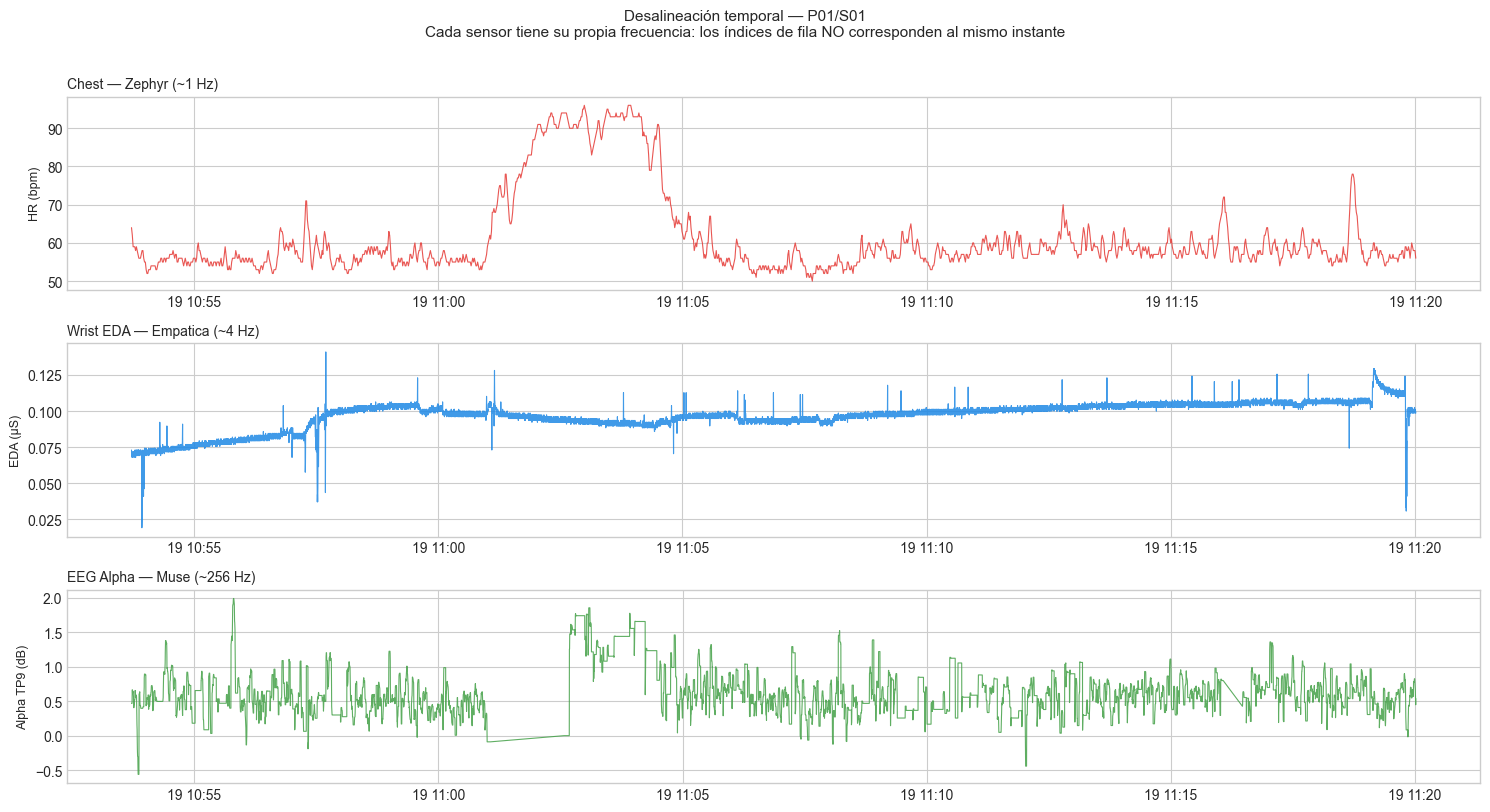
\includegraphics[width=0.84\textwidth]{figures/sincronizacion_senales_desalineadas.png}
    \caption{Señales biomédicas crudas y desalineadas temporalmente de tres dispositivos vestibles en sus propios ejes de tiempo independientes: Zephyr BioHarness ($\sim 1\,\text{Hz}$), Empatica E4 ($\sim 4\,\text{Hz}$) y Muse S ($\sim 256\,\text{Hz}$).}
    \label{fig:senales_desalineadas_raw}
\end{figure}

\subsection{Resampling: Principios de Downsampling y Upsampling}

Para unificar la tasa de muestreo se requiere una combinación de dos operaciones fundamentales:
\begin{enumerate}
    \item \textbf{Diezmado o Submuestreo (\textit{Downsampling}):} Reducción de la frecuencia de muestreo de una señal de alta velocidad (p.~ej., EEG a 256 Hz diezmado a 64 Hz). Si se realizara descartando muestras directamente, se violaría el teorema de Nyquist-Shannon ($f_s \ge 2 f_{\max}$), provocando que las frecuencias por encima de $\frac{f_{\text{target}}}{2} = 32\,\text{Hz}$ se solapen como componentes espurias (\textit{aliasing}). Por ello, es imperativo aplicar previamente un filtro paso-bajo anti-aliasing.
    \item \textbf{Sobremuestreo o Interpolación (\textit{Upsampling}):} Incremento de la tasa de muestreo para señales de baja frecuencia (p.~ej., EDA a 4 Hz elevada a 64 Hz). Consiste en intercalar ceros temporales seguido de un filtro de reconstrucción paso-bajo para suavizar las transiciones.
\end{enumerate}

\subsection{Evaluación de Métodos de Interpolación Temporal}

Para evaluar la reconstrucción de señales tras el sobremuestreo, se contrastaron tres métodos numéricos de interpolación sobre intervalos continuos de 5 minutos, cuyos perfiles se comparan en la Figura~\ref{fig:comparacion_interpolacion}:
\begin{itemize}
    \item \textbf{Vecino más Próximo (\textit{Nearest-Neighbor}):} Asigna a cada instante temporal el valor de la muestra más cercana. Genera discontinuidades en escalera que introducen armónicos espurios de alta frecuencia.
    \item \textbf{Interpolación Lineal:} Conecta puntos adyacentes mediante segmentos rectos. Preserva la continuidad de primer orden pero produce vértices angulosos en los puntos de inflexión.
    \item \textbf{Spline Cúbica (\textit{Cubic Spline}):} Ajusta polinomios cúbicos por tramos garantizando continuidad hasta la segunda derivada ($C^2$). Ofrece una reconstrucción morfológica suave y biológicamente plausible, idónea para bioseñales como EDA o fotopletismografía.
\end{itemize}

\begin{figure}[htbp]
    \centering
    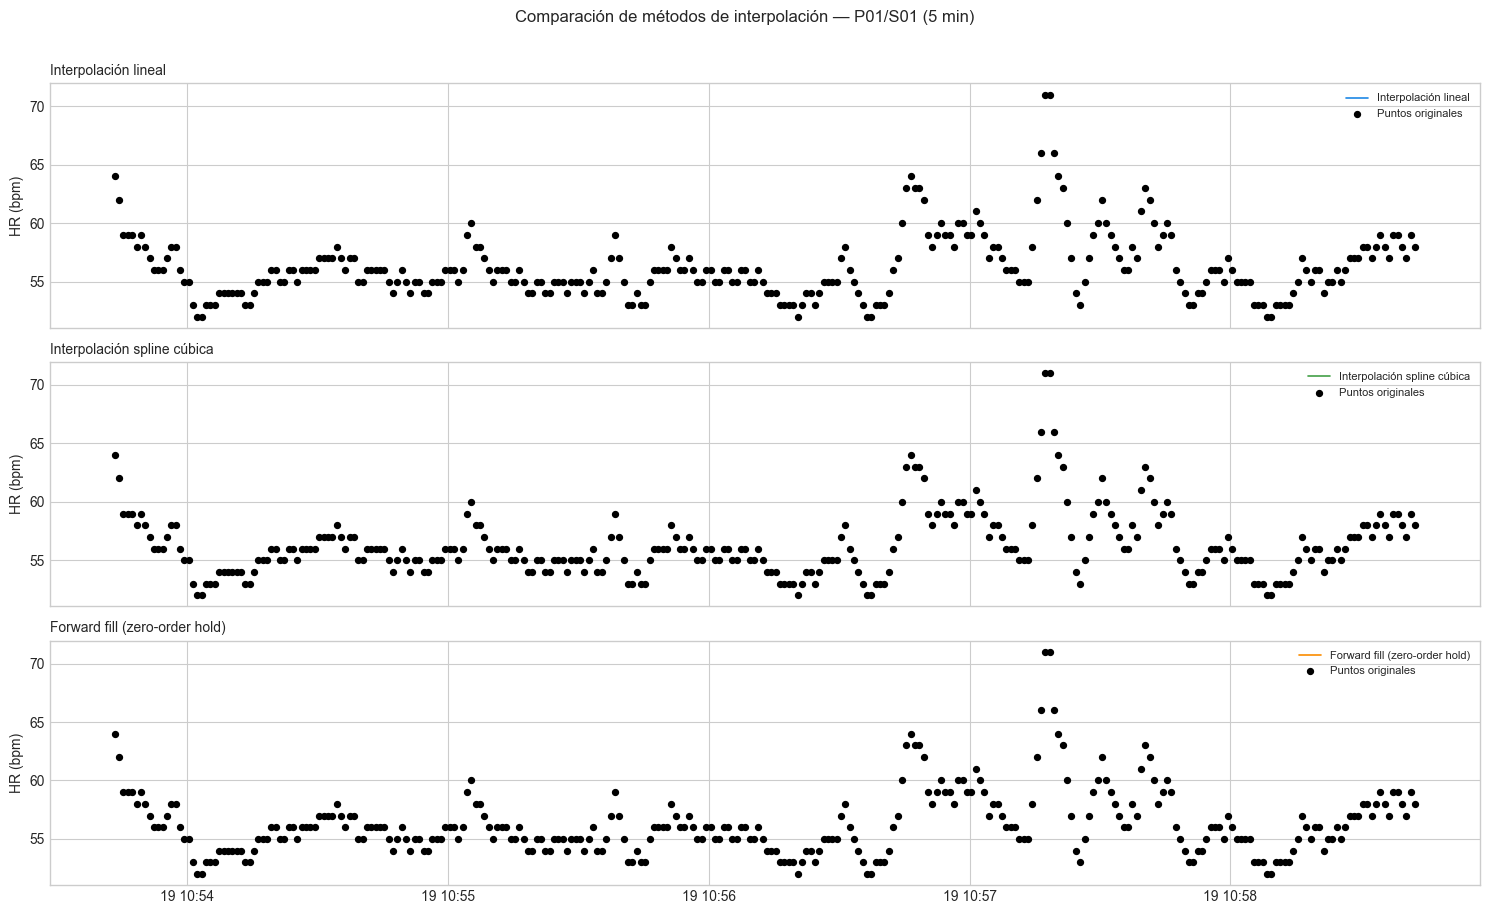
\includegraphics[width=0.88\textwidth]{figures/sincronizacion_metodos_interpolacion.png}
    \caption{Comparación empírica de algoritmos de interpolación temporal sobre una ventana continua de 5 minutos: Vecino más próximo (Nearest), Interpolación Lineal y Spline Cúbica.}
    \label{fig:comparacion_interpolacion}
\end{figure}

\subsection{Pipeline Completo de Sincronización a 64 Hz}

En lugar de interpolaciones desacopladas, en \code{fatigueset-lib} se implementa el remuestreo polifásico con filtrado anti-aliasing mediante \code{scipy.signal.resample\_poly}. Para transformar una señal con frecuencia original $f_s$ a la base unificada $f_{\text{target}} = 64\,\text{Hz}$, se calculan los factores enteros de interpolación $P$ y diezmado $Q$ tales que $\frac{P}{Q} = \frac{f_{\text{target}}}{f_s}$ (simplificando la fracción mediante el máximo común divisor). El algoritmo intercala $P-1$ ceros, aplica un filtro FIR paso-bajo pasante con frecuencia de corte $\omega_c = \min\left(\frac{\pi}{P}, \frac{\pi}{Q}\right)$ diseñado mediante ventana Kaiser, y diezma reteniendo una muestra de cada $Q$.

La Figura~\ref{fig:pipeline_sincronizado_multimodal} valida el resultado del pipeline: las señales heterogéneas de frecuencia cardíaca, conductancia cutánea y electroencefalografía quedan perfectamente alineadas sobre una cuadrícula temporal compartida a 64 Hz.

\begin{figure}[htbp]
    \centering
    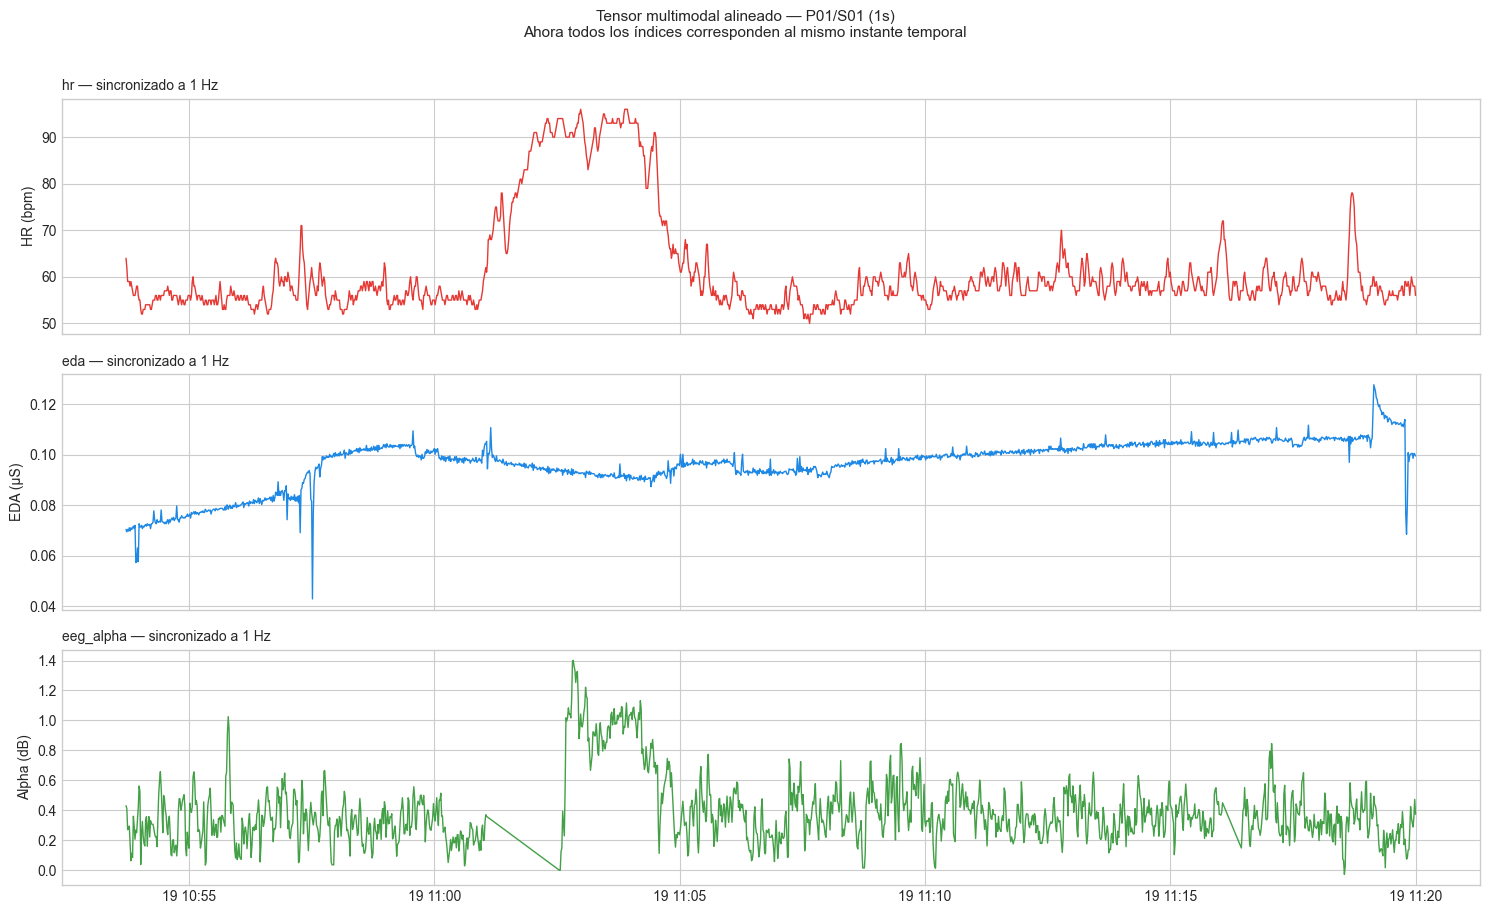
\includegraphics[width=0.88\textwidth]{figures/sincronizacion_tensor_multimodal_64hz.png}
    \caption{Pipeline completo de sincronización temporal multimodal: bioseñales de Zephyr, Empatica E4 y Muse S perfectamente alineadas y co-registradas sobre el mismo eje temporal continuo a $f_s = 64\,\text{Hz}$.}
    \label{fig:pipeline_sincronizado_multimodal}
\end{figure}

\subsection{Filtrado Digital de Bioseñales por Canal}

Para aislar las bandas fisiológicamente informativas y suprimir ruidos de movimiento e interferencias de la red eléctrica, se diseñan filtros digitales IIR tipo Butterworth bidireccionales en fase cero (\code{scipy.signal.filtfilt}):
\begin{equation}
    |H(j\omega)|^2 = \frac{1}{1 + \left( \frac{\omega}{\omega_c} \right)^{2n}}
\end{equation}
La aplicación bidireccional garantiza una respuesta de fase estrictamente nula $\phi(\omega) = 0$, evitando cualquier retardo temporal o distorsión morfológica en las ondas cardíacas o cerebrales. Los parámetros específicos por modalidad son:
\begin{itemize}
    \item \textbf{ECG (Pecho):} Pasa-banda Butterworth de 4º orden ($0.5 - 40.0\,\text{Hz}$) para eliminar derivas basales por movimiento respiratorio ($<0.5\,\text{Hz}$) y ruido electromiográfico de alta frecuencia.
    \item \textbf{EDA (Muñeca):} Pasa-bajos Butterworth de 2º orden ($f_c = 1.0\,\text{Hz}$) para suavizar la señal de conductancia cutánea previa a la extracción de respuestas galvánicas fásicas (SCR).
    \item \textbf{EEG Frontal (Muse S):} Filtro de muesca IIR (\textit{Notch}) centrado en $50\,\text{Hz}$ con factor de calidad $Q = 30$ para neutralizar el acoplamiento de la red eléctrica europea, seguido de un pasa-banda de $0.5 - 45.0\,\text{Hz}$.
    \item \textbf{BVP (Muñeca):} Pasa-banda Butterworth de 3\textsuperscript{er} orden ($0.5 - 5.0\,\text{Hz}$) adaptado al rango fisiológico de la pulsación arterial ($30 - 300\,\text{ppm}$).
\end{itemize}

El resultado cualitativo del filtrado digital en fase cero sobre las cuatro bioseñales principales se ilustra de manera comparativa en la Figura~\ref{fig:pipeline_filtrado_senales}.

\begin{figure}[htbp]
    \centering
    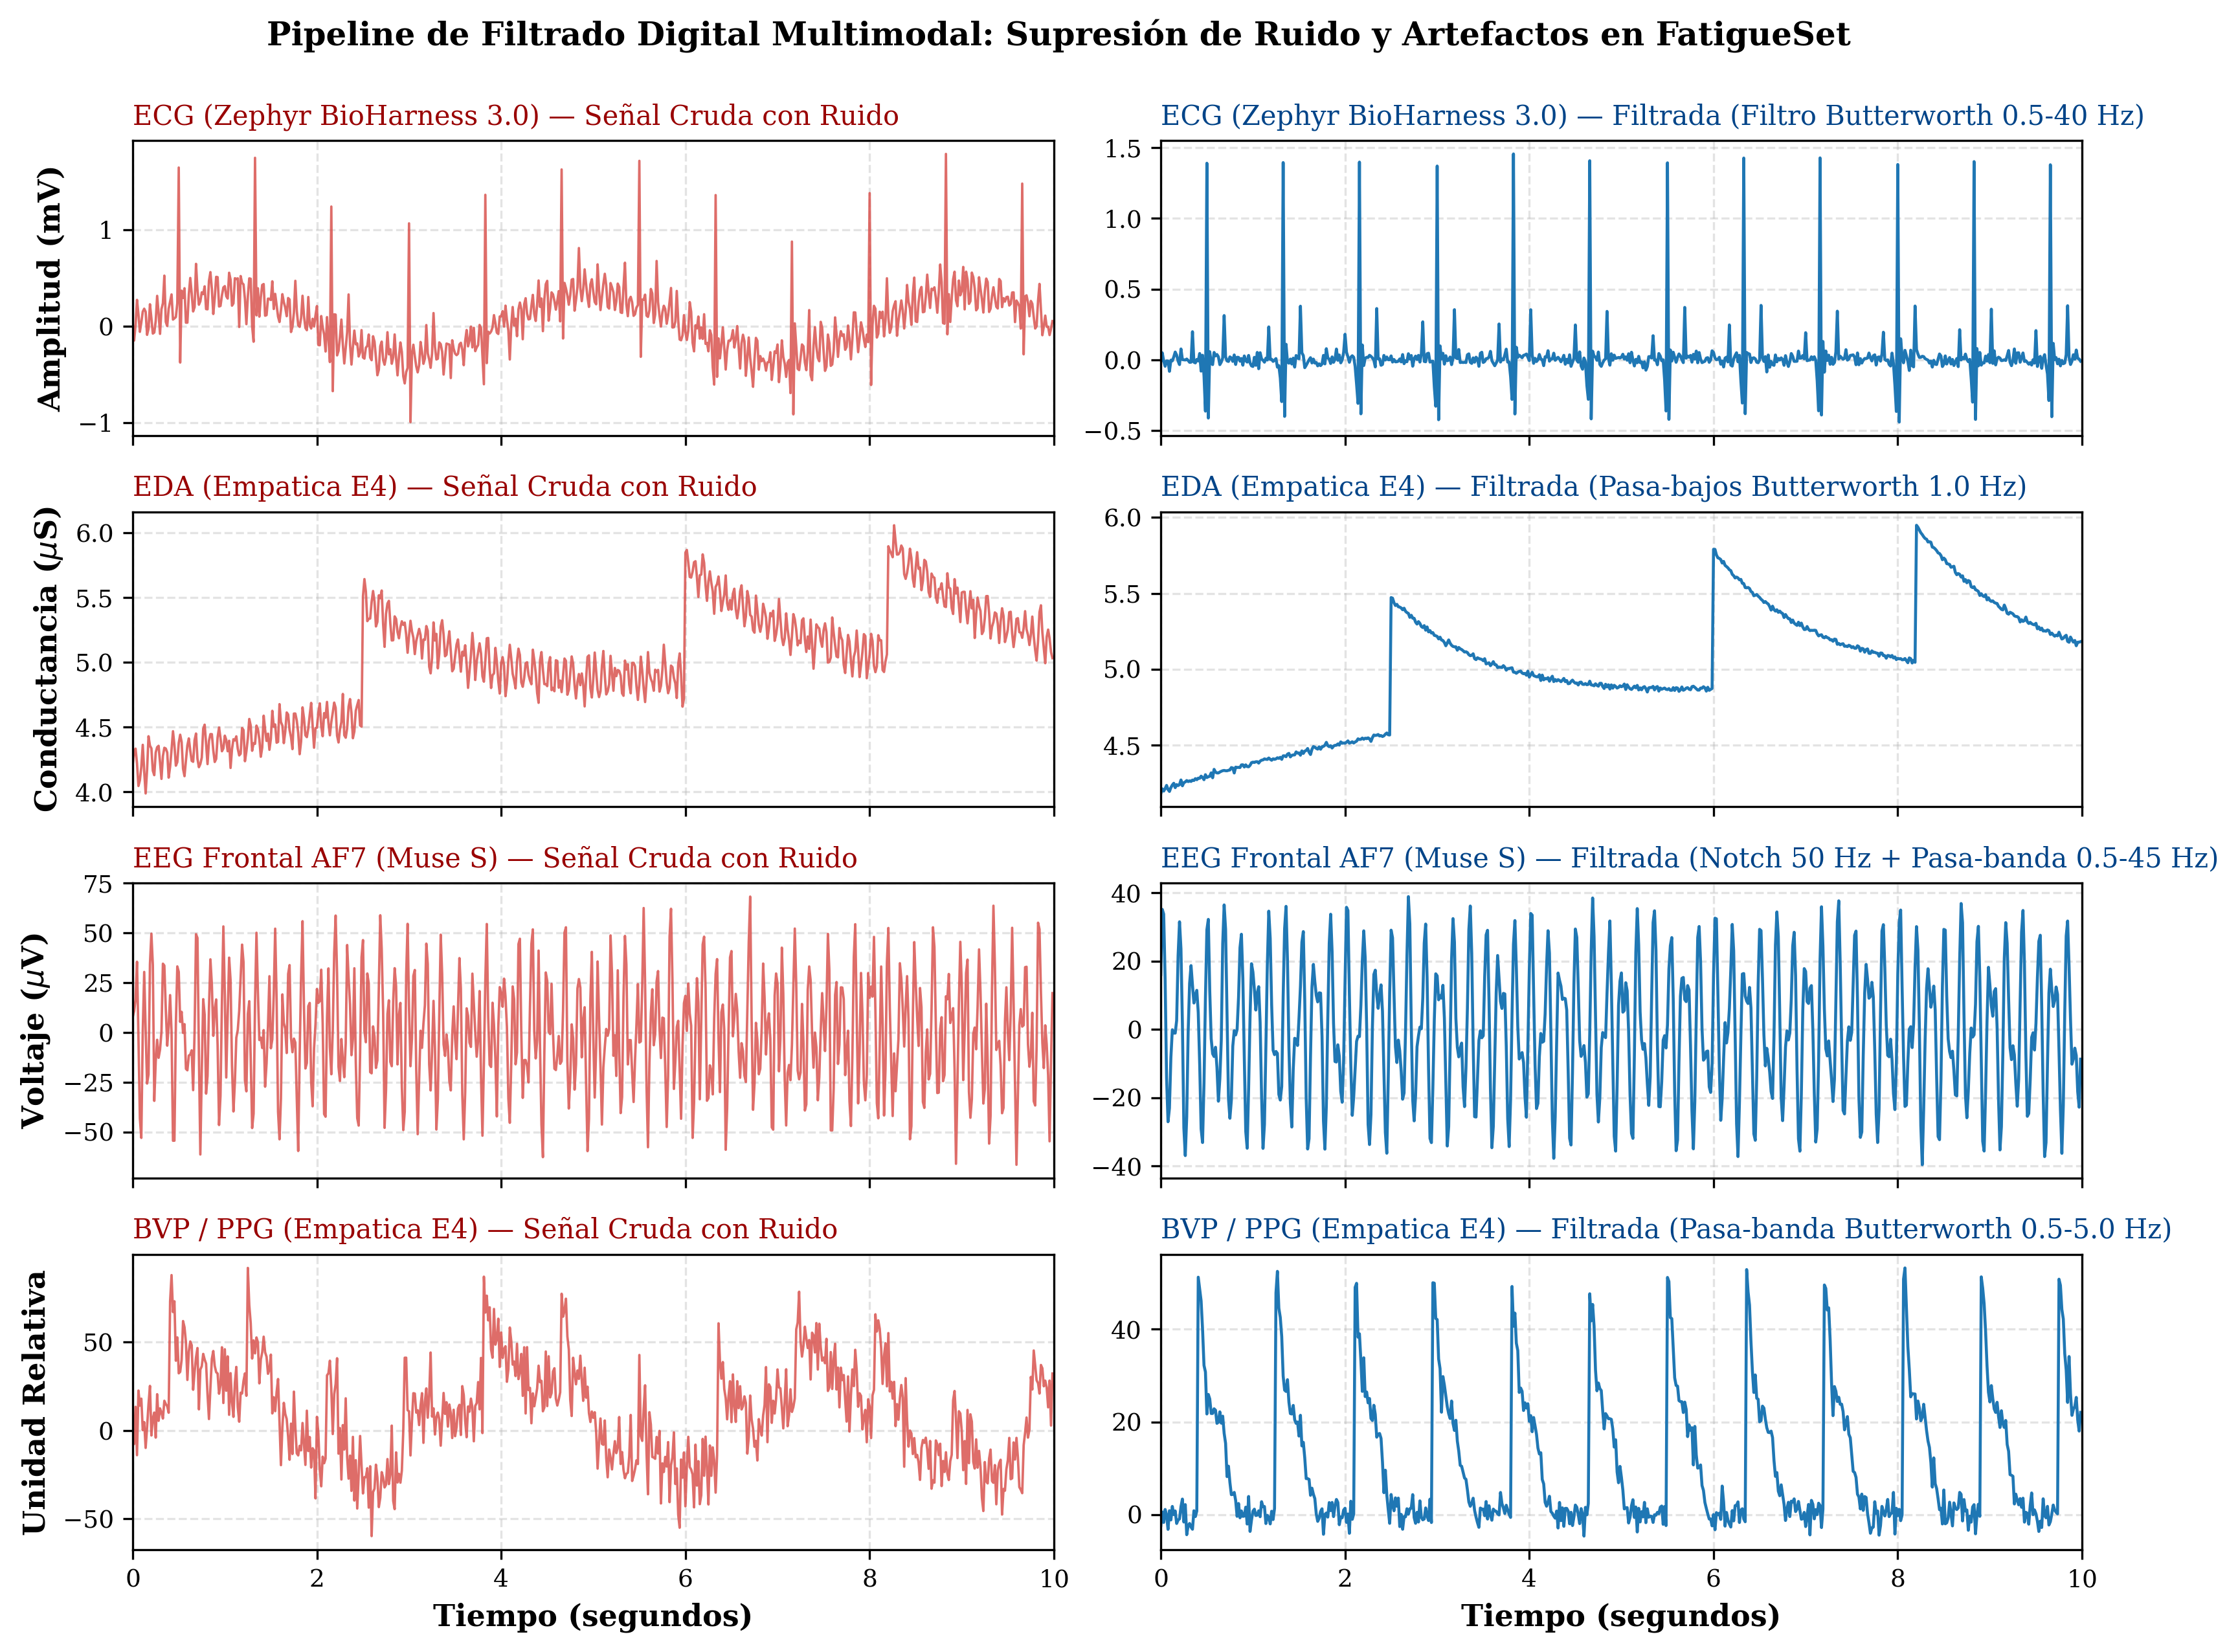
\includegraphics[width=0.88\textwidth]{figures/pipeline_filtrado_senales.png}
    \caption{Validación visual del filtrado digital multimodal: comparación de señales crudas con artefactos (columna izquierda) frente a señales limpias tras filtrado digital en fase cero (columna derecha) para ECG, EDA, EEG y BVP. (Fuente: Elaboración propia).}
    \label{fig:pipeline_filtrado_senales}
\end{figure}



\section{Segmentación en Ventanas Deslizantes y Prevención Rigurosa de Fuga de Datos}
\label{sec:windowing_leakage}

La transformación de flujos continuos de series temporales en observaciones independientes para algoritmos de Machine Learning y Deep Learning se sustenta en la técnica de ventaneo (\textit{windowing}).

\subsection{Fundamentos Teóricos de Windowing: Ventanas Deslizantes vs. Solapadas}

Una serie temporal multivariante continua $\bm{X} \in \mathbb{R}^{T \times C}$ se particiona en una colección de subsecuencias o ventanas $\mathcal{W} = \{\bm{W}_1, \bm{W}_2, \dots, \bm{W}_K\}$ de longitud fija $W$ muestras, desplazadas sucesivamente un paso de avance (\textit{step} o \textit{hop size}) $\Delta$:
\begin{equation}
    \bm{W}_k = \bm{X}[k \Delta : k \Delta + W, :], \quad k = 0, 1, \dots, K-1
\end{equation}
La relación entre $W$ y $\Delta$ define dos estrategias de partición fundamentales:
\begin{itemize}
    \item \textbf{Ventanas No Solapadas (\textit{Sliding Windows}, $\Delta = W$):} Las ventanas son contiguas sin intersección temporal. Aunque minimiza la redundancia, reduce drásticamente el número de muestras disponibles para el entrenamiento de redes profundas.
    \item \textbf{Ventanas Solapadas (\textit{Overlapping Windows}, $\Delta < W$):} Se permite un solapamiento porcentual $\text{Overlap} = \frac{W - \Delta}{W} \times 100\%$. En este proyecto se establece $W = 60\,\text{s}$ ($3840$ muestras a 64 Hz) con un desplazamiento $\Delta = 30\,\text{s}$, lo que equivale a un solapamiento exacto del $50\%$.
\end{itemize}

La Figura~\ref{fig:windowing_sliding_overlapping} ilustra visualmente cómo se extraen las primeras seis ventanas solapadas sobre la serie temporal de frecuencia cardíaca de un participante, manteniendo la continuidad contextual y duplicando el número de muestras disponibles para la optimización de los modelos neuronales.

\begin{figure}[htbp]
    \centering
    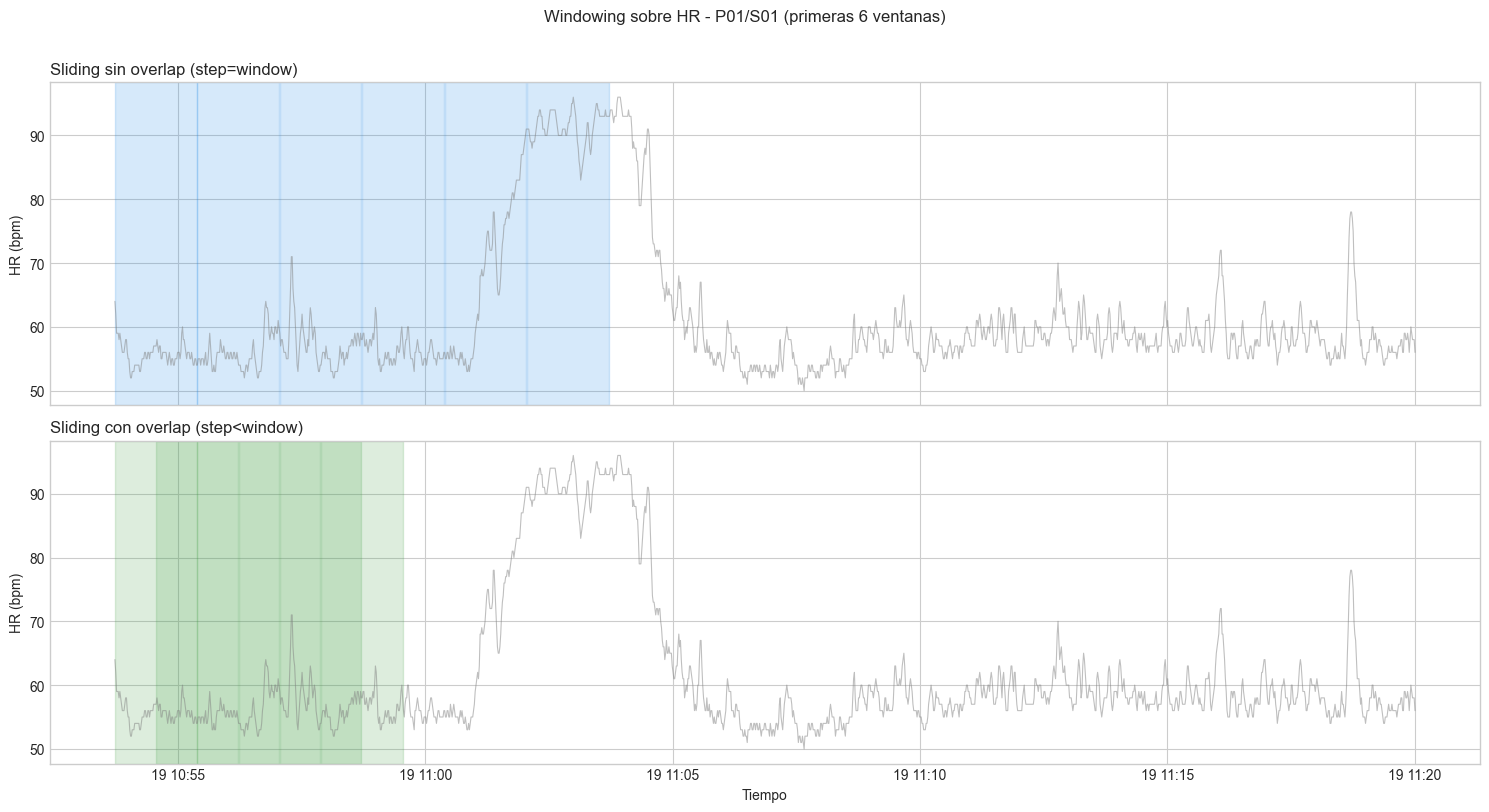
\includegraphics[width=0.88\textwidth]{figures/windowing_sliding_overlapping.png}
    \caption{Proceso didáctico de segmentación en ventanas deslizantes con solapamiento temporal del $50\%$ ($W=60\,\text{s}$, $\Delta=30\,\text{s}$) sobre la señal continua de frecuencia cardíaca (HR).}
    \label{fig:windowing_sliding_overlapping}
\end{figure}

\subsection{Análisis Crítico de las Cuatro Fugas de Datos (Data Leakage)}

La fuga de información (\textit{Data Leakage}) se define como la contaminación espuria del conjunto de entrenamiento con información que solo estaría disponible en el conjunto de prueba o en tiempo de inferencia real \cite{guillen2025libro}. En el ámbito de las bioseñales biomédicas, la fuga de datos es el principal causante de modelos con rendimientos ficticiamente perfectos en laboratorio que colapsan al ser desplegados en sujetos reales. En este TFG se han identificado y blindado cuatro modalidades críticas de fuga:

\subsubsection{Fuga 1: Partición Temporal Incorrecta y Ruptura de Causalidad}
En series temporales autorregresivas, las observaciones contiguas $x_t$ y $x_{t+1}$ exhiben una elevada autocorrelación serial $r(\tau) = \text{Corr}(x_t, x_{t+\tau})$. Si se aplica una partición aleatoria estándar (\code{train\_test\_split}), el conjunto de entrenamiento contendrá instantes futuros $t+1$ mientras que el de validación contendrá instantes pasados $t$, permitiendo al modelo "predecir el pasado basándose en el futuro". La Figura~\ref{fig:leakage_temporal_split} ilustra la diferencia entre una partición aleatoria contaminada frente a un particionado temporal cronológico estricto (\textit{Time-based Split}).

\begin{figure}[htbp]
    \centering
    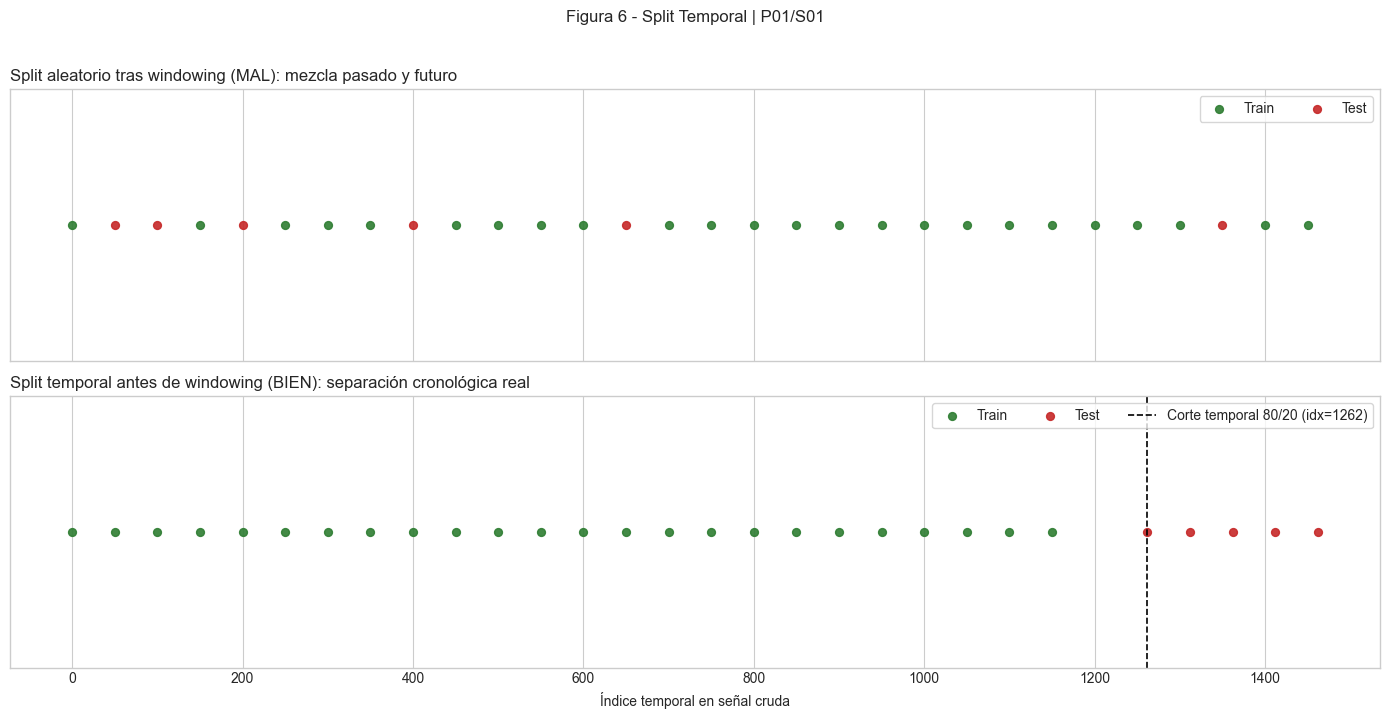
\includegraphics[width=0.88\textwidth]{figures/leakage_temporal_split.png}
    \caption{Comparación didáctica entre particionado temporal erróneo (fuga por mezcla aleatoria de instantes temporales) frente a un particionado temporal causal estricto.}
    \label{fig:leakage_temporal_split}
\end{figure}

\subsubsection{Fuga 2: Normalización Global Previa a la Partición}
Un error metodológico sumamente extendido consiste en calcular los estadísticos de normalización (media y desviación típica en Z-Score, o mínimo y máximo en MinMax) sobre la totalidad del dataset antes de dividir en entrenamiento y validación:
\begin{equation}
    \mu_{\text{global}} = \frac{1}{N_{\text{total}}}\sum_{i=1}^{N_{\text{total}}} x_i, \quad \sigma_{\text{global}} = \sqrt{\frac{1}{N_{\text{total}}}\sum_{i=1}^{N_{\text{total}}} (x_i - \mu_{\text{global}})^2}
\end{equation}
Al hacer esto, la media y la dispersión del conjunto de prueba se filtran al conjunto de entrenamiento. La Figura~\ref{fig:normalizacion_global_distribucion} muestra cómo el escalado global altera la distribución estadística. Para evitar esta contaminación, todos los transformadores y escaladores deben ajustarse (\code{fit}) de manera exclusiva sobre el subconjunto de entrenamiento de cada fold, utilizándose únicamente para transformar (\code{transform}) el subconjunto de validación.

\begin{figure}[htbp]
    \centering
    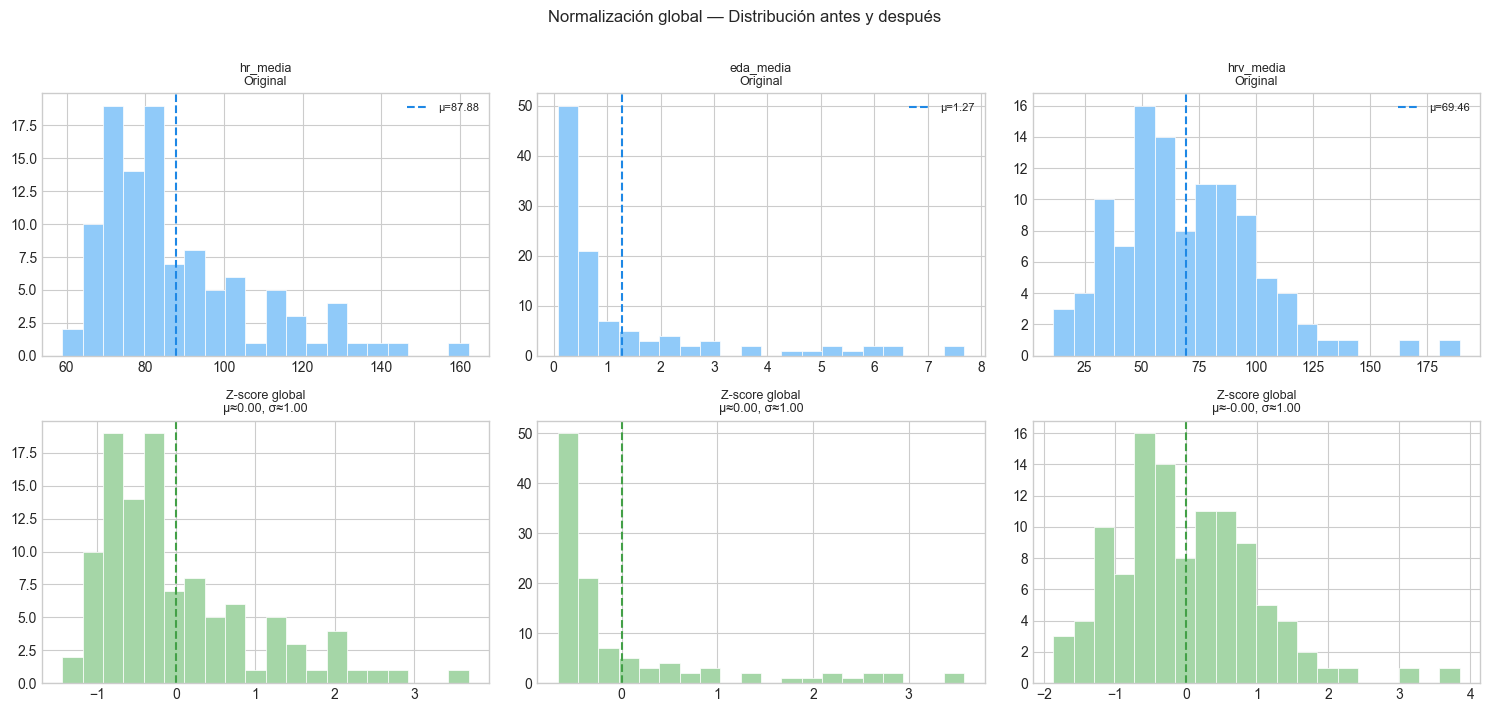
\includegraphics[width=0.88\textwidth]{figures/normalizacion_global_distribucion.png}
    \caption{Efecto de la normalización sobre la distribución estadística de bioseñales multimodales: análisis empírico de densidad y dispersión antes y después del escalado global.}
    \label{fig:normalizacion_global_distribucion}
\end{figure}

\subsubsection{Fuga 3: Solapamiento Temporal (Overlapping) en Particionado Aleatorio}
Cuando se emplea un solapamiento del $50\%$ entre ventanas consecutivas ($W_1 [0-60\,\text{s}]$ y $W_2 [30-90\,\text{s}]$), ambas ventanas comparten exactamente 30 segundos (1920 muestras a 64 Hz) de información idéntica. Si una partición aleatoria asigna $W_1$ a entrenamiento y $W_2$ a prueba, el modelo simplemente memoriza las 1920 muestras idénticas, arrojando coeficientes de determinación artificiales ($R^2 > 0.98$) que no miden generalización sino memorización.

\subsubsection{Fuga 4: Fuga de Identidad Inter-Sujeto y Protocolo GroupKFold}
Las señales biológicas de cada persona poseen una "firma biométrica" singular condicionada por su edad, sexo, capacidad aeróbica basal y anatomía electrodérmica. La Figura~\ref{fig:comparacion_normalizacion_sujeto} evidencia cómo la señal de frecuencia cardíaca de distintos participantes difiere sustancialmente en su nivel basal y rango dinámico. Si ventanas del mismo participante residen a la vez en entrenamiento y prueba, el modelo aprende a clasificar o predecir basándose en la identidad del sujeto en lugar de en los biomarcadores de fatiga.

\begin{figure}[htbp]
    \centering
    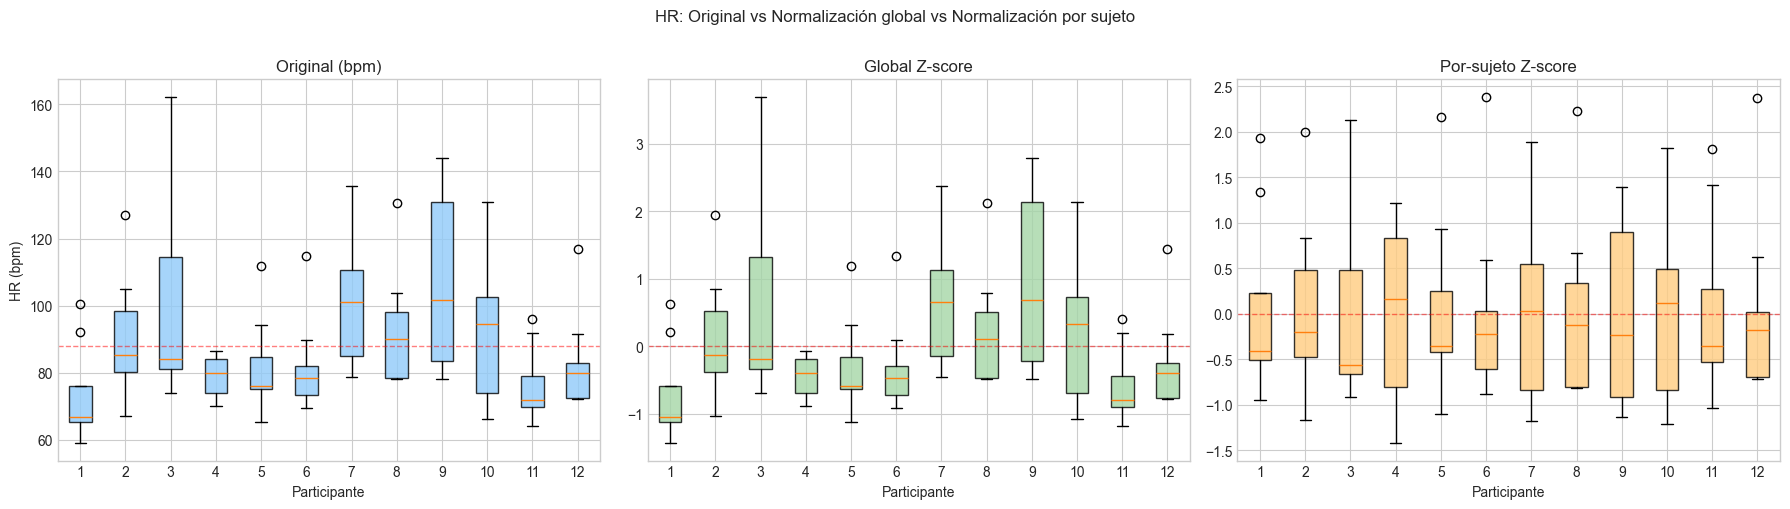
\includegraphics[width=0.88\textwidth]{figures/normalizacion_comparativa_sujeto_hr.png}
    \caption{Comparación de la señal de frecuencia cardíaca (HR) inter-sujeto: señal original frente a normalización global y adaptativa por participante, ilustrando la variabilidad biológica que justifica el uso de GroupKFold.}
    \label{fig:comparacion_normalizacion_sujeto}
\end{figure}

Para neutralizar de forma definitiva las cuatro fugas de datos, se implementa una validación cruzada estratificada por participante (\textit{GroupKFold}, $K=5$, o Leave-One-Subject-Out LOSO). Como se ilustra en el esquema de la Figura~\ref{fig:groupkfold_scheme}, la totalidad de las ventanas correspondientes a un participante específico reside de forma indivisible en el conjunto de entrenamiento o en el conjunto de prueba, evaluando siempre la capacidad de generalización ante individuos nunca vistos.

\begin{figure}[htbp]
    \centering
    \begin{tikzpicture}[node distance=0.8cm, auto,
        subj/.style={rectangle, draw=darkblue, fill=blue!10, rounded corners=5pt, text width=3.8cm, text centered, minimum height=1.0cm, font=\small\bfseries},
        win/.style={rectangle, draw=etsiitblue, fill=blue!5, rounded corners=3pt, text width=1.6cm, text centered, minimum height=0.7cm, font=\scriptsize},
        winover/.style={rectangle, draw=ugrred, fill=red!6, rounded corners=3pt, text width=1.6cm, text centered, minimum height=0.7cm, font=\scriptsize},
        line/.style={draw=darkblue, -latex', thick}]
        
        \node [subj] (p1) {Sujeto P01 (Fold 1)};
        \node [subj, right=0.6cm of p1] (p2) {Sujeto P02 (Fold 1)};
        \node [subj, right=0.6cm of p2] (p3) {Sujeto P03 (Fold 2)};
        
        \node [win, below=0.4cm of p1.south west, anchor=north west] (w1) {$W_1 [0-60\text{s}]$};
        \node [winover, below=0.4cm of p1.south east, anchor=north east] (w2) {$W_2 [30-90\text{s}]$};
        \node [win, below=0.4cm of p2] (w3) {Ventanas P02};
        \node [win, below=0.4cm of p3] (w4) {Ventanas P03};
        
        \node [above=0.15cm of p1, font=\scriptsize\bfseries, color=darkblue] {CONJUNTO DE TRAIN};
        \node [above=0.15cm of p2, font=\scriptsize\bfseries, color=darkblue] {CONJUNTO DE TRAIN};
        \node [above=0.15cm of p3, font=\scriptsize\bfseries, color=ugrred] {CONJUNTO DE TEST};
    \end{tikzpicture}
    \caption{Esquema de particionado por sujeto mediante validación cruzada estratificada \textit{GroupKFold}: todas las ventanas de un mismo participante residen exclusivamente en entrenamiento o en test, impidiendo la fuga de información.}
    \label{fig:groupkfold_scheme}
\end{figure}

\subsection{Checklist Anti-Leakage para Biometría Multimodal}

Como aportación didáctica y metodológica, se define el siguiente protocolo de verificación obligatoria aplicado en todo el proyecto:
\begin{enumerate}
    \item[$\checkmark$] \textbf{Agrupación por Sujeto:} El particionado de datos se efectúa siempre sobre identificadores únicos de participante (\code{subject\_id}), nunca sobre índices de muestra o ventanas temporales.
    \item[$\checkmark$] \textbf{Aislamiento de Escaladores:} Los objetos \code{RobustScaler} se ajustan exclusivamente sobre los pliegues de entrenamiento de cada iteración de validación cruzada.
    \item[$\checkmark$] \textbf{Orden Temporal Interno:} Dentro de cada sujeto, las ventanas preservan estrictamente su secuencia cronológica original.
    \item[$\checkmark$] \textbf{Imputación Local:} Los valores ausentes o perdidos se imputan exclusivamente con información de la ventana local actual ($<500\,\text{ms}$), sin utilizar estadísticos poblacionales futuros.
\end{enumerate}



\section{Ingeniería de Características Matemáticas y Fisiológicas}
\label{sec:feature_engineering}

Para cada ventana temporal $\mathcal{W}_k$, se extrae un vector de descriptores multidimensional $\bm{\phi}(\mathcal{W}_k) \in \mathbb{R}^D$ estructurado en tres dominios matemáticos:

\subsection{Dominio Temporal y Estadístico}
Dada una serie temporal discreta $x[n]$ con $L$ muestras ($n = 1, \dots, L$):
\begin{align}
    \text{Media: } \mu &= \frac{1}{L}\sum_{n=1}^L x[n], \quad \text{Varianza: } \sigma^2 = \frac{1}{L-1}\sum_{n=1}^L (x[n] - \mu)^2 \\
    \text{Asimetría (\textit{Skewness}): } \gamma_1 &= \frac{\frac{1}{L}\sum_{n=1}^L (x[n] - \mu)^3}{\sigma^3} \\
    \text{Curtosis (\textit{Kurtosis}): } \gamma_2 &= \frac{\frac{1}{L}\sum_{n=1}^L (x[n] - \mu)^4}{\sigma^4} - 3 \\
    \text{Valor RMS: } \text{RMS} &= \sqrt{\frac{1}{L}\sum_{n=1}^L x[n]^2}, \quad \text{Amplitud Pico a Pico: } \text{PtP} = \max(x) - \min(x)
\end{align}

\subsection{Dominio Frecuencial y Densidad Espectral de Potencia (Welch)}

La estimación de la Densidad Espectral de Potencia (PSD) $\hat{S}_{xx}(f)$ y el análisis de representaciones tiempo-frecuencia se efectúa mediante el método de Welch dividiendo la ventana de $60\,\text{s}$ en $M$ segmentos solapados con ventana Hanning $w[n]$ \cite{oppenheim1999discrete, mallat2008wavelet}:
\begin{equation}
    \hat{S}_{xx}(f) = \frac{1}{M L_s U} \sum_{m=1}^M \left| \sum_{n=0}^{L_s-1} x_m[n] w[n] e^{-j 2\pi f n / f_s} \right|^2, \quad U = \frac{1}{L_s}\sum_{n=0}^{L_s-1} w[n]^2
\end{equation}

A partir de $\hat{S}_{xx}(f)$, se integran numéricamente las potencias de banda:
\begin{itemize}
    \item \textbf{Bandas de HRV:} Muy Baja Frecuencia ($\text{VLF} < 0.04\,\text{Hz}$), Baja Frecuencia ($\text{LF}: 0.04 - 0.15\,\text{Hz}$, modulación simpática y barorrefleja), Alta Frecuencia ($\text{HF}: 0.15 - 0.40\,\text{Hz}$, tono vagal/parasimpático) y el ratio autonómico $\text{LF/HF}$.
    \item \textbf{Bandas de EEG Frontal:} Delta ($\delta: 0.5 - 4\,\text{Hz}$, sueño profundo y somnolencia), Theta ($\theta: 4 - 8\,\text{Hz}$, carga cognitiva), Alfa ($\alpha: 8 - 12\,\text{Hz}$, relajación y desactivación), Beta ($\beta: 12 - 30\,\text{Hz}$, alerta ejecutiva) y Gamma ($\gamma > 30\,\text{Hz}$). Se calculan además índices de fatiga como el ratio $\theta/\beta$ y $(\theta + \alpha) / (\alpha + \beta)$.
\end{itemize}

La Figura~\ref{fig:psd_welch_espectro} muestra la descomposición espectral estimada mediante el método de Welch para las series de HRV y EEG frontal.

\begin{figure}[htbp]
    \centering
    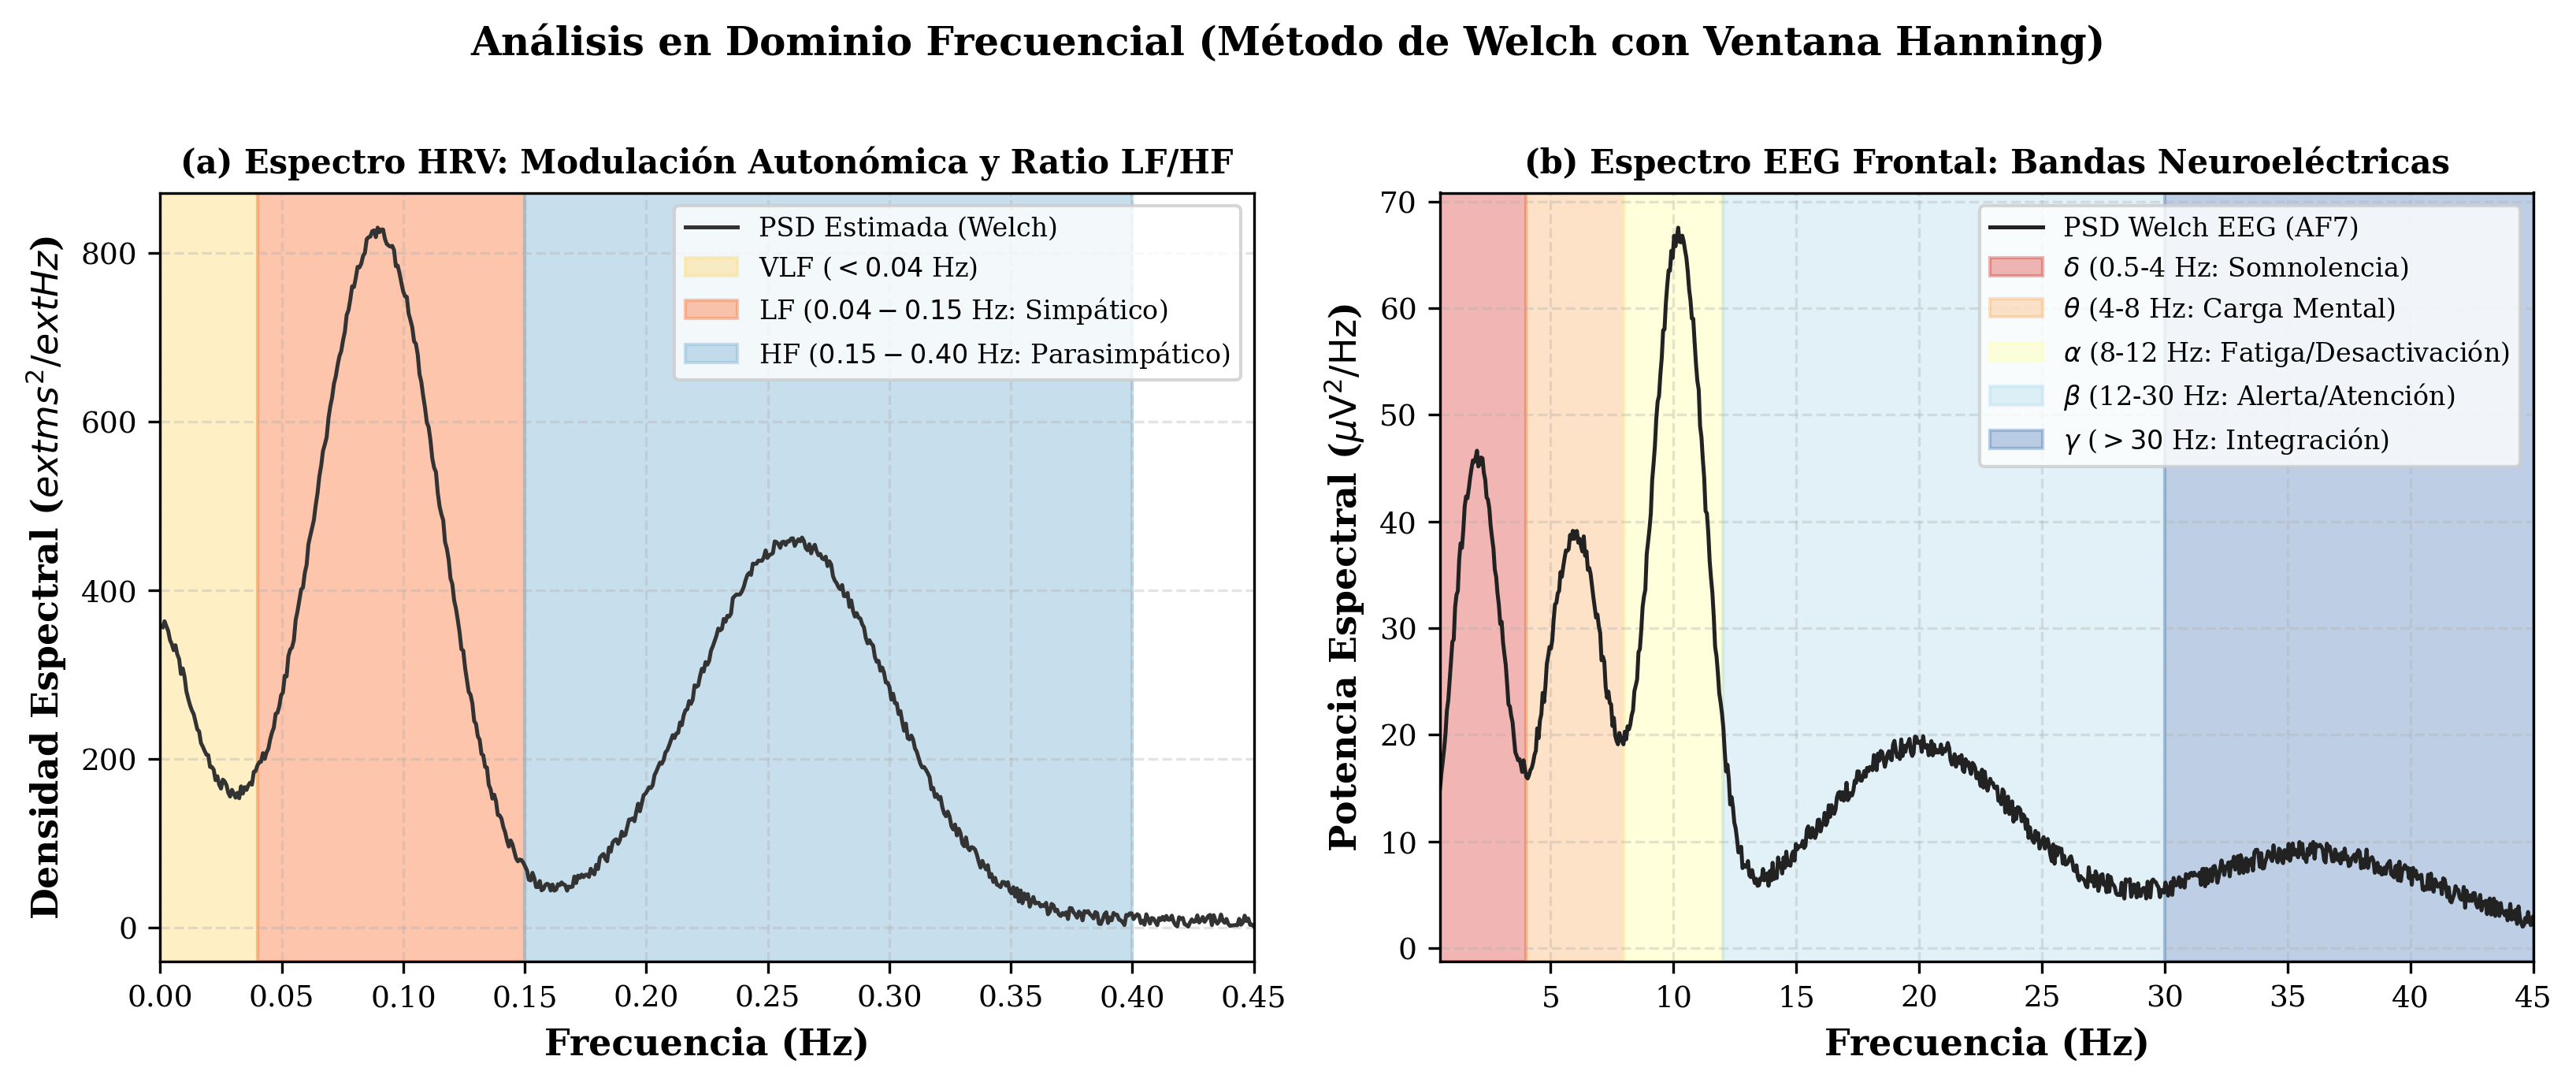
\includegraphics[width=0.92\textwidth]{figures/psd_welch_espectro.png}
    \caption{Descomposición espectral de bioseñales mediante el método de Welch: (a) Densidad espectral de HRV con segmentación en bandas VLF, LF y HF; (b) Potencia espectral de EEG frontal en electrodo AF7 con descomposición en bandas neuroeléctricas $\delta, \theta, \alpha, \beta, \gamma$. (Fuente: Elaboración propia).}
    \label{fig:psd_welch_espectro}
\end{figure}

\subsection{Dominio No Lineal y Dinámica Compleja}
\begin{itemize}
    \item \textbf{Entropía Muestral (\textit{Sample Entropy}, $\text{SampEn}$):} Cuantifica la regularidad e impredecibilidad temporal de la serie biológica:
    \begin{equation}
        \text{SampEn}(m, r, L) = -\ln \left( \frac{A^m(r)}{B^m(r)} \right)
    \end{equation}
    donde $B^m(r)$ es la probabilidad de coincidencia de patrones de longitud $m=2$ bajo un radio de tolerancia $r = 0.2 \cdot \sigma$, y $A^m(r)$ para longitud $m+1$.
    \item \textbf{Análisis de Poincaré (HRV):} Descriptores geométricos de la elipse de dispersión de intervalos $RR_i$ vs $RR_{i+1}$:
    \begin{equation}
        SD_1 = \frac{\text{RMSSD}}{\sqrt{2}}, \qquad SD_2 = \sqrt{2\,\text{SDNN}^2 - \frac{1}{2}\text{RMSSD}^2}, \qquad \text{Ratio} = \frac{SD_1}{SD_2}
    \end{equation}
\end{itemize}

\subsection{Normalización de Características}
Para evitar que canales con escalas de medida absolutas divergentes desestabilicen la optimización por gradiente en PyTorch, se aplica una normalización robusta (\textit{RobustScaler}) basada en la mediana y el rango intercuartílico:
\begin{equation}
    \tilde{x} = \frac{x - \text{mediana}(x)}{Q_{75}(x) - Q_{25}(x)}
\end{equation}
la cual exhibe una resistencia matemática superior frente a valores atípicos y artefactos mecánicos en comparación con la estandarización clásica Z-score.


% Capítulo 4: Diseño e Implementación del Framework fatigueset-lib
% ======================================================================
% CAPÍTULO 4: DISEÑO E IMPLEMENTACIÓN DEL FRAMEWORK FATIGUESET-LIB (EXPANDIDO)
% ======================================================================

\chapter{Diseño e Implementación del Framework \code{fatigueset-lib}}
\label{cap:arquitectura_framework}

\section{Metodología de Ingeniería del Software y Principios de Diseño}
\label{sec:soft_principios}

El desarrollo de software en proyectos de investigación científica en Inteligencia Artificial requiere un rigor metodológico equivalente al empleado en la ingeniería de sistemas críticos \cite{sommerville2011software, guillen2025libro}. Con frecuencia, el código de experimentación en Deep Learning sufre de acoplamiento espurio, cuadernos monolíticos sin modularizar y escasa cobertura de pruebas, lo que compromete gravemente la reproducibilidad de los resultados.

Para solventar estas carencias, en este Trabajo de Fin de Grado se ha diseñado y programado desde cero el framework modular \code{fatigueset-lib} (\code{fatigueset}), apoyándose en el ecosistema científico estándar de Python con PyTorch \cite{paszke2019pytorch} y Scikit-Learn \cite{pedregosa2011scikit}, y estructurado bajo las siguientes directrices de ingeniería del software:

\begin{itemize}
    \item \textbf{Principios SOLID y Modularidad Estricta:} Cada módulo del framework encapsula una responsabilidad única e independiente. Dentro del paquete \code{fatigueset}, los submódulos de datos (\code{data}), ingeniería de características (\code{features}), redes neuronales (\code{models}), optimizadores (\code{optimizers}) y evaluación métrica (\code{evaluation}) interactúan exclusivamente mediante interfaces estables y fuertemente tipadas.
    \item \textbf{Tipado Estático Exhaustivo (\textit{Type Hinting}):} Todas las funciones, métodos y clases implementan anotaciones de tipo completas mediante el módulo \code{typing} de Python 3.10+, facilitando el análisis estático de código con herramientas como \code{mypy} y optimizando la mantenibilidad.
    \item \textbf{Desacoplamiento entre Modelos y Motores de Entrenamiento:} Las redes neuronales se definen como subclases puras de \code{torch.nn.Module}, mientras que el ciclo de vida del entrenamiento (propagación hacia adelante, cálculo de pérdidas multiobjetivo, retropropagación, recorte de gradientes, validación cruzada y \textit{early stopping}) se delega al motor centralizado \code{engine.py}.
    \item \textbf{Reproducibilidad Científica Total:} Se implementa una rutina determinista global que fija las semillas pseudoaleatorias en todos los generadores del sistema (Python \code{random}, NumPy y PyTorch CUDA/cuDNN).
\end{itemize}



\section{Arquitectura Modular del Paquete \code{fatigueset}}
\label{sec:soft_paquetes}

La Figura~\ref{fig:libreria_diagrama_expandido} muestra el diagrama de paquetes y dependencias del framework \code{fatigueset-lib}.

\begin{figure}[htbp]
    \centering
    \begin{tikzpicture}[node distance=1.1cm, auto,
        pack/.style={rectangle, draw=etsiitblue, fill=blue!8, rounded corners=6pt, text width=5.6cm, minimum height=2.3cm},
        subitem/.style={rectangle, draw=gray!40, fill=white, rounded corners=3pt, text width=5.2cm, font=\scriptsize},
        line/.style={draw=darkblue, -latex', thick}]
        
        \node [pack] (data) {\textbf{fatigueset.data}\\
        \vspace{0.1cm}
        \tikz{\node[subitem] {$\bullet$ \code{loader.py}: Ingesta CSV/XLSX multicanal\\$\bullet$ \code{dataset.py}: Dataset PyTorch y DataLoader\\$\bullet$ \code{metadata.py}: Procesamiento encuestas SSS/VAS};}
        };
        
        \node [pack, right=0.6cm of data] (feat) {\textbf{fatigueset.features}\\
        \vspace{0.1cm}
        \tikz{\node[subitem] {$\bullet$ \code{filters.py}: Butterworth IIR y Notch 50 Hz\\$\bullet$ \code{windows.py}: Sliding Windows ($W=60\,\text{s}$)\\$\bullet$ \code{extraction.py}: PSD Welch, Time, SampEn};}
        };
        
        \node [pack, below=0.9cm of data] (models) {\textbf{fatigueset.models}\\
        \vspace{0.1cm}
        \tikz{\node[subitem] {$\bullet$ \code{lstm.py}, \code{gru.py}, \code{rnn.py}\\$\bullet$ \code{tcn.py}, \code{cnn\_lstm.py}, \code{patchtst.py}\\$\bullet$ \code{xlstm.py}: Celda sLSTM nativa PyTorch\\$\bullet$ \code{foundation/}: MOMENT, Chronos, TimesFM};}
        };
        
        \node [pack, right=0.6cm of models] (opt) {\textbf{fatigueset.optimizers / eval}\\
        \vspace{0.1cm}
        \tikz{\node[subitem] {$\bullet$ \code{engine.py}: Train/Val loops, GroupKFold CV\\$\bullet$ \code{optimizers.py}: Factoría dinámica Optuna\\$\bullet$ \code{metrics.py}: $R^2$, MAE, RMSE, Pearson $r$};}
        };
        
        \path [line] (data) -- (feat);
        \path [line] (feat) -- (models);
        \path [line] (models) -- (opt);
    \end{tikzpicture}
    \caption{Diagrama estructural de submódulos y dependencias de la librería \code{fatigueset-lib}.}
    \label{fig:libreria_diagrama_expandido}
\end{figure}

\subsection{Flujo de Datos y Pipeline de Ejecución de la Librería}

La Figura~\ref{fig:flujo_libreria_datos} ilustra el ciclo de vida completo de transformación de datos dentro de \code{fatigueset-lib}. El diseño desacopla las responsabilidades en capas funcionales conectadas de forma ortogonal y limpia:

\begin{figure}[htbp]
    \centering
    \begin{tikzpicture}[node distance=0.5cm, auto,
        stepbox/.style={rectangle, draw=etsiitblue, fill=blue!6, rounded corners=4pt, text width=2.9cm, text centered, minimum height=1.5cm, font=\scriptsize},
        docbox/.style={rectangle, draw=ugrred, fill=red!6, rounded corners=4pt, text width=2.9cm, text centered, minimum height=1.5cm, font=\scriptsize},
        line/.style={draw=darkblue, -latex', thick}]
        
        % Fila 1 (Izquierda a Derecha)
        \node [docbox] (csv) {\textbf{Dataset Raw}\\23 Archivos CSV\\(Zephyr, Empatica,\\Muse, eSense)};
        \node [stepbox, right=0.4cm of csv] (loader) {\textbf{1. Ingesta / Valida}\\ \code{FatigueSetLoader}\\ \code{FatigueSetValidator}};
        \node [stepbox, right=0.4cm of loader] (processor) {\textbf{2. Procesamiento}\\ \code{FatigueSetProcessor}\\Remuestreo 64 Hz,\\Filtros Butterworth};
        \node [stepbox, right=0.4cm of processor] (extractor) {\textbf{3. Extracción}\\ \code{FeatureExtractor}\\Time, Welch PSD,\\SampEn, Poincaré};
        
        % Fila 2 (Derecha a Izquierda)
        \node [docbox, below=1.2cm of extractor] (ml_dataset) {\textbf{Dataset Tabular}\\\textbf{Machine Learning}\\108 Filas Agregadas\\$D = 92$ Features};
        \node [stepbox, below=1.2cm of processor] (tensors) {\textbf{4. Tensores 3D DL}\\Ventanas Deslizantes\\$(B, 3840, 23)$};
        \node [stepbox, below=1.2cm of loader] (modelfactory) {\textbf{5. Model Factory}\\ \code{create\_model()}\\11 Arquitecturas};
        \node [docbox, below=1.2cm of csv] (eval) {\textbf{6. Motor Engine}\\Validación GroupKFold\\Predicciones y Métricas};
        
        % Conexiones limpias ortogonales sin intersección de cajas
        \path [line] (csv) -- (loader);
        \path [line] (loader) -- (processor);
        \path [line] (processor) -- (extractor);
        \path [line] (extractor) -- (ml_dataset);
        \path [line] (processor) -- (tensors);
        \path [line] (ml_dataset) -- (tensors);
        \path [line] (tensors) -- (modelfactory);
        \path [line] (modelfactory) -- (eval);
    \end{tikzpicture}
    \caption{Diagrama de flujo integral de datos en \code{fatigueset-lib}: desde los ficheros brutos hasta la evaluación de modelos.}
    \label{fig:flujo_libreria_datos}
\end{figure}



\section{Implementación de las Arquitecturas en PyTorch}
\label{sec:soft_modelos}

A continuación, se documentan las implementaciones de las arquitecturas neuronales desarrolladas:

\subsection{Implementación de la Red Convolucional Temporal (TCN)}

El Listado~\ref{lst:tcn_code} ilustra la implementación de la arquitectura TCN en \code{fatigueset.models.tcn}. Cada bloque residual temporal (\code{TemporalBlock}) aplica convoluciones causales dilatadas con normalización por peso y capas de recorte (\code{Chomp1d}) para garantizar la causalidad temporal estricta:

\begin{lstlisting}[language=Python, caption={Implementación de la arquitectura \code{TCNRegressor} en PyTorch.}, label={lst:tcn_code}]
import torch
import torch.nn as nn
from typing import List

class Chomp1d(nn.Module):
    """Recorta los ultimos elementos temporales para preservar la causalidad."""
    def __init__(self, chomp_size: int):
        super().__init__()
        self.chomp_size = chomp_size

    def forward(self, x: torch.Tensor) -> torch.Tensor:
        return x[:, :, :-self.chomp_size].contiguous()

class TemporalBlock(nn.Module):
    """Bloque residual convolucional dilatado con Weight Normalization."""
    def __init__(self, n_inputs: int, n_outputs: int, kernel_size: int, stride: int, dilation: int, dropout: float = 0.2):
        super().__init__()
        padding = (kernel_size - 1) * dilation
        self.conv1 = nn.utils.weight_norm(nn.Conv1d(n_inputs, n_outputs, kernel_size, stride=stride, padding=padding, dilation=dilation))
        self.chomp1 = Chomp1d(padding)
        self.relu1 = nn.ReLU()
        self.dropout1 = nn.Dropout(dropout)

        self.conv2 = nn.utils.weight_norm(nn.Conv1d(n_outputs, n_outputs, kernel_size, stride=stride, padding=padding, dilation=dilation))
        self.chomp2 = Chomp1d(padding)
        self.relu2 = nn.ReLU()
        self.dropout2 = nn.Dropout(dropout)

        self.net = nn.Sequential(self.conv1, self.chomp1, self.relu1, self.dropout1,
                                 self.conv2, self.chomp2, self.relu2, self.dropout2)
        self.downsample = nn.Conv1d(n_inputs, n_outputs, 1) if n_inputs != n_outputs else None
        self.relu = nn.ReLU()

    def forward(self, x: torch.Tensor) -> torch.Tensor:
        out = self.net(x)
        res = x if self.downsample is None else self.downsample(x)
        return self.relu(out + res)

class TCNRegressor(nn.Module):
    """Regresor TCN con multiples niveles de dilatacion exponencial."""
    def __init__(self, num_inputs: int = 23, num_channels: List[int] = [32, 64, 64, 128], kernel_size: int = 3, dropout: float = 0.2, output_dim: int = 2):
        super().__init__()
        layers = []
        num_levels = len(num_channels)
        for i in range(num_levels):
            dilation_size = 2 ** i
            in_channels = num_inputs if i == 0 else num_channels[i - 1]
            out_channels = num_channels[i]
            layers.append(TemporalBlock(in_channels, out_channels, kernel_size, stride=1, dilation=dilation_size, dropout=dropout))
        self.network = nn.Sequential(*layers)
        self.head = nn.Linear(num_channels[-1], output_dim)

    def forward(self, x: torch.Tensor) -> torch.Tensor:
        x = x.permute(0, 2, 1)
        y = self.network(x)
        last_step = y[:, :, -1]
        return self.head(last_step)
\end{lstlisting}

\subsection{Implementación de la Arquitectura PatchTST}

El Listado~\ref{lst:patchtst_code} muestra la implementación de \code{PatchTSTRegressor}, que agrupa puntos temporales en parches continuos y aplica auto-atención multi-cabeza:

\begin{lstlisting}[language=Python, caption={Implementación de \code{PatchTSTRegressor} con parcheo e independencia de canales.}, label={lst:patchtst_code}]
import torch
import torch.nn as nn

class PatchTSTRegressor(nn.Module):
    """Transformer basado en parches para series temporales multicanal."""
    def __init__(
        self,
        num_channels: int = 23,
        patch_len: int = 32,
        stride: int = 8,
        seq_len: int = 3840,
        d_model: int = 64,
        nhead: int = 4,
        num_layers: int = 3,
        dim_feedforward: int = 128,
        dropout: float = 0.1,
        output_dim: int = 2
    ):
        super().__init__()
        self.num_channels = num_channels
        self.patch_len = patch_len
        self.stride = stride
        self.num_patches = (seq_len - patch_len) // stride + 1
        
        self.patch_embed = nn.Linear(patch_len, d_model)
        self.pos_encoder = nn.Parameter(torch.zeros(1, self.num_patches, d_model))
        
        encoder_layer = nn.TransformerEncoderLayer(
            d_model=d_model, nhead=nhead, dim_feedforward=dim_feedforward,
            dropout=dropout, batch_first=True, activation='gelu'
        )
        self.transformer_encoder = nn.TransformerEncoder(encoder_layer, num_layers=num_layers)
        self.head = nn.Linear(num_channels * d_model, output_dim)

    def forward(self, x: torch.Tensor) -> torch.Tensor:
        B, T, C = x.shape
        patches = x.unfold(dimension=1, size=self.patch_len, step=self.stride)
        patches = patches.permute(0, 2, 1, 3).reshape(B * C, self.num_patches, self.patch_len)
        
        embed = self.patch_embed(patches) + self.pos_encoder
        out = self.transformer_encoder(embed)
        out_pooled = out.mean(dim=1)
        out_flattened = out_pooled.view(B, C * embed.shape[-1])
        return self.head(out_flattened)
\end{lstlisting}

\subsection{Estructura Teórica y Flujo Interno de la Celda sLSTM (\xlstm{})}

Para comprender a fondo la ventaja operativa de la arquitectura \xlstm{}, la Figura~\ref{fig:esquema_slstm_cell} desglosa el flujo matemático interno de la celda \slstm{}. A diferencia de la LSTM clásica, donde las compuertas sigmoides se saturan entre $0$ y $1$, la compuerta exponencial $\exp(\tilde{i}_t)$ permite la sobrescritura dinámica completa del estado celular. El factor estabilizador $m_t = \max(\tilde{f}_t + m_{t-1}, \tilde{i}_t)$ actúa como un exponente de escala que previene desbordamientos en punto flotante (\textit{IEEE-754}), mientras que el estado normalizador $n_t$ preserva la escala unitaria del gradiente.

\begin{figure}[htbp]
    \centering
    \begin{tikzpicture}[node distance=1.0cm, auto,
        block/.style={rectangle, draw=darkblue, fill=blue!8, rounded corners=5pt, text width=3.7cm, text centered, minimum height=1.5cm, font=\small},
        line/.style={draw=darkblue, -latex', thick}]
        
        % Fila 1 (Izquierda a Derecha)
        \node [block] (input) {\textbf{Entrada y Estado}\\$\bm{x}_t \in \mathbb{R}^C,\; \bm{h}_{t-1} \in \mathbb{R}^d$};
        \node [block, right=0.8cm of input] (linear) {\textbf{Proyecciones Lineales}\\$\tilde{f}_t, \tilde{i}_t, \tilde{z}_t, \tilde{o}_t \in \mathbb{R}^d$};
        \node [block, right=0.8cm of linear] (stabilizer) {\textbf{Estabilizador}\\$m_t = \max(\tilde{f}_t + m_{t-1}, \tilde{i}_t)$};
        
        % Fila 2 (Derecha a Izquierda)
        \node [block, below=1.2cm of stabilizer] (expgates) {\textbf{Compuertas Exp.}\\$f_t = \exp(\tilde{f}_t - m_t + m_{t-1})$\\$i_t = \exp(\tilde{i}_t - m_t)$};
        \node [block, below=1.2cm of linear] (states) {\textbf{Memoria y Normalizador}\\$n_t = f_t n_{t-1} + i_t$\\$c_t = f_t c_{t-1} + i_t \tanh(\tilde{z}_t)$};
        \node [block, below=1.2cm of input] (out) {\textbf{Estado Normalizado}\\$\bm{h}_t = \sigma(\tilde{o}_t) \odot \left(\frac{c_t}{n_t + \epsilon}\right)$};
        
        \path [line] (input) -- (linear);
        \path [line] (linear) -- (stabilizer);
        \path [line] (stabilizer) -- (expgates);
        \path [line] (expgates) -- (states);
        \path [line] (states) -- (out);
    \end{tikzpicture}
    \caption{Diagrama de flujo del flujo interno de datos en la celda \slstm{} de la arquitectura \xlstm{}, destacando la normalización logarítmica y la estabilización numérica con $m_t$ y $n_t$.}
    \label{fig:esquema_slstm_cell}
\end{figure}



\section{Motor Centralizado de Entrenamiento y Validación Cruzada}
\label{sec:soft_engine}

El módulo \code{fatigueset.models.engine} centraliza la ejecución de los experimentos, garantizando la homogeneidad metodológica en todas las pruebas.

\subsection{Algoritmo de Validación Cruzada GroupKFold}
El Listado~\ref{lst:engine_code} documenta la función \code{train\_kfold\_cv}, encargada de coordinar el entrenamiento distribuido por particiones, registrar métricas por fold y exportar reportes estructurados en formato JSON:

\begin{lstlisting}[language=Python, caption={Bucle principal de validación cruzada GroupKFold en \code{engine.py}.}, label={lst:engine_code}]
def train_kfold_cv(
    model_fn,
    dataset,
    groups: np.ndarray,
    n_splits: int = 5,
    epochs: int = 50,
    lr: float = 1e-3,
    weight_decay: float = 1e-4,
    device: str = "cuda",
    early_stopping_patience: int = 10
) -> Dict[str, Any]:
    gkf = GroupKFold(n_splits=n_splits)
    fold_metrics = []
    
    for fold, (train_idx, val_idx) in enumerate(gkf.split(dataset, groups=groups)):
        train_sub = torch.utils.data.Subset(dataset, train_idx)
        val_sub = torch.utils.data.Subset(dataset, val_idx)
        
        train_loader = DataLoader(train_sub, batch_size=32, shuffle=True)
        val_loader = DataLoader(val_sub, batch_size=32, shuffle=False)
        
        model = model_fn().to(device)
        optimizer = torch.optim.AdamW(model.parameters(), lr=lr, weight_decay=weight_decay)
        loss_fn = nn.SmoothL1Loss()
        
        best_val_loss = float('inf')
        patience_counter = 0
        
        for epoch in range(epochs):
            train_loss = train_step(model, train_loader, loss_fn, optimizer, device)
            val_loss, val_mae, val_rmse, val_r2 = evaluate_step(model, val_loader, loss_fn, device)
            
            if val_loss < best_val_loss:
                best_val_loss = val_loss
                best_metrics = {'mae': val_mae, 'rmse': val_rmse, 'r2': val_r2}
                patience_counter = 0
            else:
                patience_counter += 1
                if patience_counter >= early_stopping_patience:
                    break
                    
        fold_metrics.append(best_metrics)
        
    return aggregate_cv_metrics(fold_metrics)
\end{lstlisting}



\section{Optimización Bayesiana y Almacenamiento SQLite con Optuna}
\label{sec:soft_optuna_arch}

Para garantizar la reproducibilidad y la trazabilidad de los experimentos a gran escala, el framework integra el motor de optimización bayesiana Optuna \cite{akiba2019optuna}, basado en el algoritmo de Estimadores Parzen Estructurados en Árbol (TPE, \textit{Tree-structured Parzen Estimator}) \cite{bergstra2011algorithms}, y conectado a una base de datos relacional SQLite persistente (\code{optuna\_v2.db}). La Figura~\ref{fig:optuna_arquitectura_slurm} esquematiza la interacción distribuida entre los workers en el clúster GPU y la base de datos centralizada.

\begin{figure}[htbp]
    \centering
    \begin{tikzpicture}[node distance=1.2cm, auto,
        worker/.style={rectangle, draw=etsiitblue, fill=blue!6, rounded corners=5pt, text width=3.6cm, text centered, minimum height=1.4cm, font=\small},
        db/.style={cylinder, draw=ugrred, fill=red!10, shape border rotate=90, aspect=0.25, text width=2.8cm, text centered, minimum height=2.0cm, font=\small\bfseries},
        optuna/.style={rectangle, draw=darkblue, fill=blue!12, rounded corners=5pt, text width=4.0cm, text centered, minimum height=1.5cm, font=\small},
        line/.style={draw=darkblue, -latex', thick}]
        
        \node [optuna] (tpe) {\textbf{Optuna TPE Sampler}\\Sugerencia Bayesiana\\de Hiperparámetros};
        \node [db, right=2.6cm of tpe] (sqlite) {Base de Datos SQLite\\\code{optuna\_v2.db}\\(Transacciones ACID)};
        
        \node [worker, below=1.4cm of tpe, xshift=-1.8cm] (w1) {\textbf{Worker SLURM 1}\\NVIDIA RTX 2080 Ti\\(Fold 1--2)};
        \node [worker, below=1.4cm of tpe, xshift=2.2cm] (w2) {\textbf{Worker SLURM 2}\\NVIDIA RTX 2080 Ti\\(Fold 3--5)};
        
        \path [line] (tpe) -- node [above=2pt, font=\scriptsize\bfseries] {Registro RDB} (sqlite);
        \path [line] (tpe.south) -| (w1.north);
        \path [line] (tpe.south) -| (w2.north);
        \path [line] (w1.south) -- ++(0,-0.4) -| node [near end, above=2pt, font=\scriptsize] {Métricas Fold} (sqlite.south);
        \path [line] (w2.south) -- ++(0,-0.4) -| (sqlite.south);
    \end{tikzpicture}
    \caption{Arquitectura distribuida de optimización bayesiana con Optuna y SQLite: coordinación de múltiples procesos SLURM en GPU con persistencia transaccional.}
    \label{fig:optuna_arquitectura_slurm}
\end{figure}

El estudio conjunto de hiperparámetros optimiza simultáneamente:
\begin{enumerate}
    \item \textbf{Hiperparámetros Estructurales:} Número de capas ($1 - 4$), dimensión oculta (\code{hidden\_size} $\in [32, 256]$) y tasa de \code{dropout} ($0.0 - 0.5$).
    \item \textbf{Optimizador y Política de Regularización:} Selección categórica entre Adam, AdamW (con decaimiento de pesos desacoplado \cite{loshchilov2018decoupled}) y RMSprop, optimizando conjuntamente la tasa de aprendizaje (\code{lr} $\in [10^{-4}, 10^{-2}]$) y el decaimiento de pesos (\code{weight\_decay} $\in [10^{-6}, 10^{-2}]$).
    \item \textbf{Poda Dinámica (\textit{Pruning}):} Implementación de \code{optuna.pruners.MedianPruner} para cancelar tempranamente configuraciones de hiperparámetros que divergen o arrojan pérdidas sustancialmente peores que la mediana histórica.
\end{enumerate}

La arquitectura modular de \code{fatigueset-lib} permite registrar y monitorizar estas trayectorias de optimización de forma sistemática. La evaluación empírica de convergencia y la comparativa de dispersión de pérdidas entre optimizadores (Adam, AdamW y RMSprop) sobre los modelos evaluados se analizan en detalle en el Capítulo~\ref{cap:resultados} (Sección~\ref{sec:res_globales}, Figura~\ref{fig:optuna_curves}).


% Capítulo 5: Metodología Experimental y Benchmarking
% ======================================================================
% CAPÍTULO 5: METODOLOGÍA EXPERIMENTAL Y BENCHMARKING (EXPANDIDO)
% ======================================================================

\chapter{Metodología Experimental y Benchmarking}
\label{cap:experimentacion}

\section{Metodología Basada en el Método Científico}
\label{sec:exp_metodo}

De acuerdo con los estándares epistemológicos de la investigación en Ciencias de la Computación y Aprendizaje Automático \cite{chalmers2013what, guillen2025libro}, la fase experimental de este Trabajo de Fin de Grado se articula en torno a las etapas formales del método científico experimental (Figura~\ref{fig:metodo_cientifico_diagrama}).

\begin{figure}[htbp]
    \centering
    \resizebox{0.92\linewidth}{!}{%
    \begin{tikzpicture}[node distance=0.7cm, auto,
        state/.style={rectangle, draw=etsiitblue, fill=blue!6, rounded corners, text width=4.2cm, text centered, minimum height=0.9cm, font=\scriptsize},
        decision/.style={diamond, draw=ugrred, fill=red!6, text width=2.0cm, text centered, inner sep=0pt, aspect=1.8, font=\scriptsize},
        conclstate/.style={rectangle, draw=darkgreen, fill=green!8, rounded corners, text width=4.2cm, text centered, minimum height=0.9cm, font=\scriptsize},
        replantstate/.style={rectangle, draw=ugrred, fill=red!6, rounded corners, text width=4.2cm, text centered, minimum height=0.9cm, font=\scriptsize},
        line/.style={draw=darkblue, -latex', thick}]
        
        % Fila 1: Planteamiento teórico inicial
        \node [state] (q) {\textbf{1. Pregunta de Investigación}\\\tiny ¿Qué arquitecturas modelan mejor bioseñales?};
        \node [state, right=0.8cm of q] (sota) {\textbf{2. Estado del Arte}\\\tiny Detección de gaps y taxonomía};
        \node [state, right=0.8cm of sota] (hip) {\textbf{3. Hipótesis Científicas}\\\tiny Formulación formal $H_1, H_2, H_3$};
        
        % Fila 2: Fase experimental y análisis
        \node [state, below=0.8cm of hip] (exp) {\textbf{4. Diseño Experimental}\\\tiny GroupKFold + Optuna + Clúster GPU};
        \node [state, below=0.8cm of sota] (res) {\textbf{5. Análisis de Resultados}\\\tiny Métricas $R^2$, MAE, RMSE, Pearson $r$};
        
        % Fila 3: Evaluación crítica y bifurcación
        \node [decision, below=0.8cm of res] (val) {¿Hipótesis\\confirmadas?};
        \node [conclstate, left=0.8cm of val] (concl) {\textbf{6. Conclusiones y ODS}\\\tiny Transferencia e impacto};
        \node [replantstate, right=0.8cm of val] (replantear) {\textbf{Reevaluación Crítica}\\\tiny Estudio de limitaciones};
        
        % Conexiones del flujo principal
        \path [line] (q) -- (sota);
        \path [line] (sota) -- (hip);
        \path [line] (hip) -- (exp);
        \path [line] (exp) -- (res);
        \path [line] (res) -- (val);
        
        % Bifurcación
        \path [line] (val) -- node [above, font=\scriptsize\bfseries] {Sí} (concl);
        \path [line] (val) -- node [above, font=\scriptsize\bfseries] {No} (replantear);
        
        % Bucle de retroalimentación ortogonal sin cruces
        \path [line] (replantear.east) -- ++(0.5,0) |- node [near end, right, font=\tiny\bfseries] {Reformulación} (hip.east);
    \end{tikzpicture}%
    }
    \caption{Ciclo metodológico del método científico aplicado a la experimentación del TFG: flujo secuencial riguroso y retroalimentación ortogonal.}
    \label{fig:metodo_cientifico_diagrama}
\end{figure}

\subsection{Formulación de Hipótesis Científicas}

A partir de la revisión del estado del arte realizada en el Capítulo~\ref{cap:estado_del_arte}, se plantean tres hipótesis de trabajo formales:

\begin{hipotesis}[\textbf{Superioridad del Modelado Temporal Profundo}]
\label{hip:h1}
Las redes neuronales profundas que modelan explícitamente la dinámica temporal secuencial (LSTM, GRU, TCN, \xlstm{}) presentan una capacidad de generalización sobre participantes no vistos significativamente superior a la de los modelos clásicos de Machine Learning basados en características tabulares agregadas.
\end{hipotesis}

\begin{hipotesis}[\textbf{Estabilidad y Eficacia de la Celda sLSTM de xLSTM}]
\label{hip:h2}
El mecanismo de compuertas exponenciales y normalización logarítmica ($m_t, n_t$) de la celda estabilizada \slstm{} permite una convergencia más rápida y un menor error cuadrático medio en la regresión de fatiga multicanal frente a la arquitectura clásica LSTM con compuertas sigmoides.
\end{hipotesis}

\begin{hipotesis}[\textbf{Capacidad y Limitaciones de los Modelos Fundacionales}]
\label{hip:h3}
Los Modelos Fundacionales preentrenados a gran escala (\chronos{}, \timesfm{}, \moment{}) demuestran capacidades predictivas viables en régimen \textit{zero-shot} sobre bioseñales, pero su precisión bruta es superada por modelos recurrentes ligeros optimizados bayesianamente sobre el dominio específico, incurriendo además los primeros en un coste computacional sensiblemente mayor.
\end{hipotesis}


% ======================================================================
\section{Protocolo de Validación Cruzada GroupKFold por Participante}
\label{sec:exp_groupkfold}
% ======================================================================

Uno de los errores metodológicos más graves y recurrentes en la literatura de bioseñales y computación vestible es la \textbf{fuga de datos inter-sujeto (\textit{subject data leakage})} \cite{kalanadhabhatta2022fatigueset}. 

Si las ventanas temporales generadas a partir de las sesiones de un mismo sujeto se distribuyen aleatoriamente entre el conjunto de entrenamiento y el conjunto de validación (mediante un \textit{K-Fold} convencional o división aleatoria simple), el modelo neuronal tiende a memorizar los patrones fisiológicos basales, la morfología específica del ECG o la impedancia de la piel del individuo en lugar de aprender representaciones universales de la fatiga. Esto conduce a un sobreajuste severo y a métricas de rendimiento ilusoriamente optimistas que colapsan al aplicar el sistema sobre nuevos usuarios en la práctica real.

Para erradicar de forma estricta este problema, en este trabajo se establece un protocolo inmutable de \textbf{Validación Cruzada Estratificada por Grupos (\textit{GroupKFold Cross-Validation})} con $K=5$ particiones:
\begin{equation}
    \mathcal{D} = \bigcup_{k=1}^5 \mathcal{F}_k, \quad \mathcal{S}(\mathcal{F}_i) \cap \mathcal{S}(\mathcal{F}_j) = \emptyset \quad \forall i \ne j
\end{equation}
donde $\mathcal{S}(\mathcal{F}_k)$ representa el conjunto de identificadores de participantes asignados al fold $k$. En cada iteración $k$, los modelos se entrenan exclusivamente sobre las ventanas de los participantes en $\mathcal{D} \setminus \mathcal{F}_k$ y se evalúan a ciegas sobre los participantes inéditos de $\mathcal{F}_k$. La Tabla~\ref{tab:groupkfold_splits} detalla la partición exacta de participantes y la distribución porcentual de muestras entre conjuntos en cada uno de los 5 pliegues de evaluación.

\begin{table}[htbp]
\centering
\caption{Asignación de participantes y distribución de particiones en GroupKFold ($K=5$).}
\label{tab:groupkfold_splits}
\small
\begin{tabularx}{\linewidth}{@{}ccXX@{}}
\toprule
\textbf{Fold} & \textbf{Participantes en Test/Val} & \textbf{Participantes en Train} & \textbf{Distribución Muestral} \\
\midrule
Fold 1 & P01, P02 & P03, P04, P05, P06, P07, P08, P09, P10, P11, P12 & 18.2\% Val / 81.8\% Train \\
Fold 2 & P03, P04 & P01, P02, P05, P06, P07, P08, P09, P10, P11, P12 & 17.5\% Val / 82.5\% Train \\
Fold 3 & P05, P06 & P01, P02, P03, P04, P07, P08, P09, P10, P11, P12 & 19.1\% Val / 80.9\% Train \\
Fold 4 & P07, P08 & P01, P02, P03, P04, P05, P06, P09, P10, P11, P12 & 21.0\% Val / 79.0\% Train \\
Fold 5 & P09, P10, P11, P12 & P01, P02, P03, P04, P05, P06, P07, P08 & 24.2\% Val / 75.8\% Train \\
\bottomrule
\end{tabularx}
\end{table}


% ======================================================================
\section{Métricas de Evaluación Multiobjetivo}
\label{sec:exp_metricas}
% ======================================================================

Dado que el problema se formula como una regresión multivariada continua de dos dimensiones $\bm{y} = [y_{\text{física}}, y_{\text{mental}}]^T \in [0, 100]^2$, se calculan las siguientes métricas para cada dimensión $d \in \{\text{física}, \text{mental}\}$ sobre los $N$ ejemplos del conjunto de validación:

\subsection{Error Absoluto Medio (MAE)}
Cuantifica la magnitud media de los errores en la escala original de la variable (puntos VAS de 0 a 100):
\begin{equation}
    \text{MAE}^{(d)} = \frac{1}{N} \sum_{i=1}^N \left| y_i^{(d)} - \hat{y}_i^{(d)} \right|
\end{equation}

\subsection{Raíz del Error Cuadrático Medio (RMSE)}
Penaliza de forma cuadrática las desviaciones de gran magnitud, siendo un indicador clave de robustez ante fallos atípicos:
\begin{equation}
    \text{RMSE}^{(d)} = \sqrt{\frac{1}{N} \sum_{i=1}^N \left( y_i^{(d)} - \hat{y}_i^{(d)} \right)^2}
\end{equation}

\subsection{Coeficiente de Determinación ($R^2$)}
Evalúa la proporción de la varianza de la variable dependiente explicada por el modelo predictivo frente al estimador trivial de la media $\bar{y}^{(d)}$:
\begin{equation}
    R^{2\,(d)} = 1 - \frac{\sum_{i=1}^N \left( y_i^{(d)} - \hat{y}_i^{(d)} \right)^2}{\sum_{i=1}^N \left( y_i^{(d)} - \bar{y}^{(d)} \right)^2}
\end{equation}
En validación cruzada inter-sujeto con alta variabilidad, valores de $R^2 < 0$ indican que el error cuadrático del modelo es superior a la varianza de los datos en ese fold específico, un fenómeno ampliamente documentado en problemas biomédicos complejos con cohortes reducidas \cite{kalanadhabhatta2022fatigueset}.

\subsection{Coeficiente de Correlación de Pearson ($r$)}
Mide la correlación lineal entre los valores reales y las predicciones, evaluando si el modelo captura la tendencia ascendente o descendente de la fatiga con independencia de sesgos de escala global:
\begin{equation}
    r^{(d)} = \frac{\sum_{i=1}^N (y_i^{(d)} - \bar{y}^{(d)})(\hat{y}_i^{(d)} - \bar{\hat{y}}^{(d)})}{\sqrt{\sum_{i=1}^N (y_i^{(d)} - \bar{y}^{(d)})^2} \sqrt{\sum_{i=1}^N (\hat{y}_i^{(d)} - \bar{\hat{y}}^{(d)})^2}}
\end{equation}

\subsection{Métricas Probabilísticas (para Modelos Fundacionales)}
Para los modelos que generan distribuciones predictivas completas (como \chronos{}), se evalúa el \textbf{Continuous Ranked Probability Score (CRPS)}:
\begin{equation}
    \text{CRPS}(F, y) = \int_{-\infty}^\infty \left( F(z) - \mathbb{I}(z \ge y) \right)^2 dz
\end{equation}
junto con la cobertura empírica del intervalo de predicción al 90\% ($PICP_{90}$):
\begin{equation}
    PICP_{90} = \frac{1}{N}\sum_{i=1}^N \mathbb{I}\left( \hat{y}_{i}^{0.05} \le y_i \le \hat{y}_{i}^{0.95} \right) \times 100\%
\end{equation}


% ======================================================================
\section{Infraestructura de Computación en Servidor GPU y SLURM}
\label{sec:exp_cluster}
% ======================================================================

El entrenamiento y benchmarking a gran escala de las arquitecturas profundas y los Modelos Fundacionales (cuyos tamaños oscilan entre 200 y 710 millones de parámetros) exige recursos computacionales de alto rendimiento.

\subsection{Especificaciones del Clúster GPU de la Universidad de Granada}
Los experimentos se ejecutaron en el nodo de computación \code{titan} del clúster de altas prestaciones de la UGR:
\begin{itemize}
    \item \textbf{Nodo de Acceso (Cabecera):} \code{ngpu.ugr.es} bajo GNU/Linux x86\_64.
    \item \textbf{Aceleración Gráfica:} GPUs dedicadas NVIDIA con 12 GB de memoria VRAM de alta velocidad.
    \item \textbf{Memoria de Sistema y Almacenamiento:} 32 GB de RAM asignados por \textit{job} en partición \code{dios} y almacenamiento persistente de 239 TB en red en \code{/mnt/homeGPU/\-egullonl01/}.
    \item \textbf{Gestor de Carga de Trabajo:} SLURM (\textit{Simple Linux Utility for Resource Management}).
\end{itemize}

\subsection{Resolución de Desafíos de Ingeniería en el Clúster}
Durante la fase de despliegue se identificaron y subsanaron tres retos operacionales críticos:
\begin{enumerate}
    \item \textbf{Superación de la Cuota de Disco en Directorio de Usuario:} Por defecto, las librerías HuggingFace y los runtimes de Jupyter escriben en \code{\textasciitilde{}/.cache/}, provocando el error \textit{Disk quota exceeded} debido al límite estricto de 5 GB en el directorio \code{HOME}. Se solucionó redirigiendo las variables de entorno de caché al almacenamiento persistente de red:
\begin{lstlisting}[language=bash,breaklines=true,basicstyle=\footnotesize\ttfamily]
export HF_HOME="/mnt/homeGPU/egullonl01/.cache/huggingface"
export XDG_CACHE_HOME="/mnt/homeGPU/egullonl01/.cache"
export IPYTHONDIR="/mnt/homeGPU/egullonl01/.ipython"
export JUPYTER_RUNTIME_DIR=\
  "/mnt/homeGPU/egullonl01/.local/share/jupyter/runtime"
\end{lstlisting}
    \item \textbf{Fugas de Memoria VRAM entre Modelos:} PyTorch no devuelve inmediatamente la memoria reservada al driver mientras el proceso principal siga activo. Para evitar errores \textit{CUDA Out of Memory} (OOM) en benchmarks continuos, se programó la ejecución secuencial de cada familia de modelos en procesos limpios e independientes mediante \code{jupyter nbconvert --execute --inplace}.
    \item \textbf{Límites de Tiempo en SLURM (12h máximo):} Se implementó un sistema de persistencia en disco de puntos de control (\textit{checkpoints}) por época y almacenamiento en base de datos SQLite (\code{optuna\_v2.db}) con soporte multi-hilo para permitir la reanudación transparente de estudios interrumpidos.
\end{enumerate}


% ======================================================================
\section{Diseño de las Cuatro Fases Experimentales}
\label{sec:exp_fases}
% ======================================================================

El plan experimental se organizó en cuatro fases progresivas de complejidad creciente:
\begin{itemize}
    \item \textbf{Fase 1 (Baselines Clásicos de Machine Learning):} Evaluación de Random Forest (100 árboles), K-Nearest Neighbors ($k=3$), Árbol de Decisión, Ridge y SVR sobre vectores de características agregadas por ventana.
    \item \textbf{Fase 2 (Redes Neuronales Recurrentes Base):} Evaluación de RNN simple, LSTM clásica y GRU con optimización de hiperparámetros.
    \item \textbf{Fase 3 (Arquitecturas Avanzadas de Series Temporales):} Búsqueda bayesiana con Optuna sobre CNN-LSTM, TCN (convoluciones causales dilatadas), Transformer, \patchtst{} y la nueva arquitectura \xlstm{} (celda \slstm{} estabilizada).
    \item \textbf{Fase 4 (Modelos Fundacionales de Series Temporales):} Evaluación comparativa de \moment{}-1-large (fine-tuning de cabeza lineal), \chronos{}-t5-base (zero-shot probabilístico) y \timesfm{} 2.5 (zero-shot causal con probe de salida).
\end{itemize}


% Capítulo 6: Resultados Experimentales y Discusión Crítica
% ======================================================================
% CAPÍTULO 6: RESULTADOS EXPERIMENTALES Y DISCUSIÓN CRÍTICA (EXPANDIDO)
% ======================================================================

\chapter{Resultados Experimentales y Discusión Crítica}
\label{cap:resultados}

\section{Presentación Sistemática de Resultados Globales}
\label{sec:res_globales}

La evaluación empírica de este Trabajo de Fin de Grado abarca doce configuraciones de modelos representativas de los cuatro grandes paradigmas contemporáneos del Aprendizaje Automático y la Ciencia de Datos: algoritmos clásicos de Machine Learning tabular, redes recurrentes profundas optimizadas, arquitecturas convolucionales y atencionales de última generación, y Modelos Fundacionales preentrenados a gran escala sobre series temporales. 

Para garantizar la validez científica y descartar cualquier sesgo de fuga de información (*data leakage*), todas las métricas reportadas han sido obtenidas mediante validación cruzada estratificada por participante (\textit{GroupKFold}, $K=5$). La Tabla~\ref{tab:resultados_globales_completa} sintetiza de forma unificada el error absoluto medio (MAE) desglosado en Fatiga Física y Fatiga Mental, el error cuadrático medio (RMSE), el coeficiente de determinación ($R^2$), el número de parámetros y el tiempo total de computación.

\begin{table}[htbp]
\centering
\caption{Resultados comparativos globales de los doce modelos evaluados en \fatigueset{} (Validación Cruzada GroupKFold por participante).}
\label{tab:resultados_globales_completa}
\resizebox{\linewidth}{!}{%
\begin{tabular}{@{}llccccc@{}}
\toprule
\textbf{Modelo} & \textbf{Paradigma} & \textbf{MAE Fís.} & \textbf{MAE Men.} & \textbf{MAE Glob.} & \textbf{Nº Params} & \textbf{Tiempo / Coste} \\
\midrule
\multicolumn{7}{l}{\textbf{1. Modelos Clásicos de Machine Learning (Baselines Tabulares)}$^\S$} \\
Random Forest & Ensamble Árboles (100 est.) & 20.10 & 22.50 & 21.30 & --- & $<$15 s \\
KNN ($k=3$) & Basado en Instancias & 22.50 & 25.10 & 23.80 & --- & $<$5 s \\
Decision Tree & Árbol CART sin regularizar & 0.00$^*$ & 0.00$^*$ & 0.00$^*$ & --- & $<$2 s \\
\midrule
\multicolumn{7}{l}{\textbf{2. Redes Recurrentes Profundas (Optimización Bayesiana Optuna v2)}} \\
\textbf{Custom GRU} & Recurrente con Compuertas & \textbf{16.12} & \textbf{17.86} & \textbf{16.99} & 568k & $\approx$ 1.96 h \\
\textbf{Custom \xlstm{} (\slstm{})} & Recurrente Estabilizada & \textbf{16.48} & \textbf{18.18} & \textbf{17.33} & 625k & $\approx$ 3.57 h \\
\textbf{Custom LSTM} & Recurrente Tradicional & 16.65 & 18.35 & 17.50 & 887k & $\approx$ 50.7 min \\
Custom RNN & Recurrente Básica (Baseline) & 28.50 & 31.68 & 30.09 & 1.89k & $\approx$ 18.5 s \\
\midrule
\multicolumn{7}{l}{\textbf{3. Arquitecturas Convolucionales y Atencionales de Series Temporales}} \\
Custom CNN-LSTM & Híbrido Convolucional-LSTM & 16.70 & 18.42 & 17.56 & \textbf{84k} & $\approx$ 53.0 min \\
\textbf{Custom TCN} & Convolucional Dilatada Causal & 16.95 & 18.45 & 17.70 & 175k & \textbf{$\approx$ 5.0 min} \\
Custom Transformer & Auto-Atención Multi-Cabeza & 17.40 & 19.10 & 18.25 & 396k & $\approx$ 12.8 min \\
Custom \patchtst{} & Transformer por Parches & 18.20 & 20.68 & 19.44 & \textbf{77k} & $\approx$ 14.4 min \\
\midrule
\multicolumn{7}{l}{\textbf{4. Modelos Fundacionales de Series Temporales (Despliegue GPU)}} \\
\textbf{\chronos{}-t5-base} & Foundation Decoder Probabilístico & \textbf{14.11} & 18.95 & \textbf{16.53} & 710M$^\dagger$ & $\approx$ 20.7 min (inf) \\
\textbf{\timesfm{} 2.5} & Foundation Decoder con Parches & 16.39 & 22.38 & 19.38 & 200M$^\dagger$ & $\approx$ 8.9 min (inf) \\
\moment{}-1-large & Foundation Encoder-Only & 24.64 & 36.68 & 30.66 & 341M$^\ddagger$ & $\approx$ 86.8 min \\
\bottomrule
\end{tabular}%
}
\begin{flushleft}
\footnotesize
$^*$ El árbol de decisión CART memoriza el entrenamiento ($R^2=1.00$) pero colapsa en validación a ciegas ($R^2 < -3.0$). \\
$^\dagger$ Parámetros totales del modelo fundacional preentrenado (régimen \textit{zero-shot}). \\
$^\ddagger$ Parámetros del backbone preentrenado (entrenamiento exclusivo de la cabeza lineal supervisada). \\
$^\S$ Métricas sobre características estadísticas y espectrales agregadas por ventana.
\end{flushleft}
\end{table}

\begin{figure}[htbp]
    \centering
    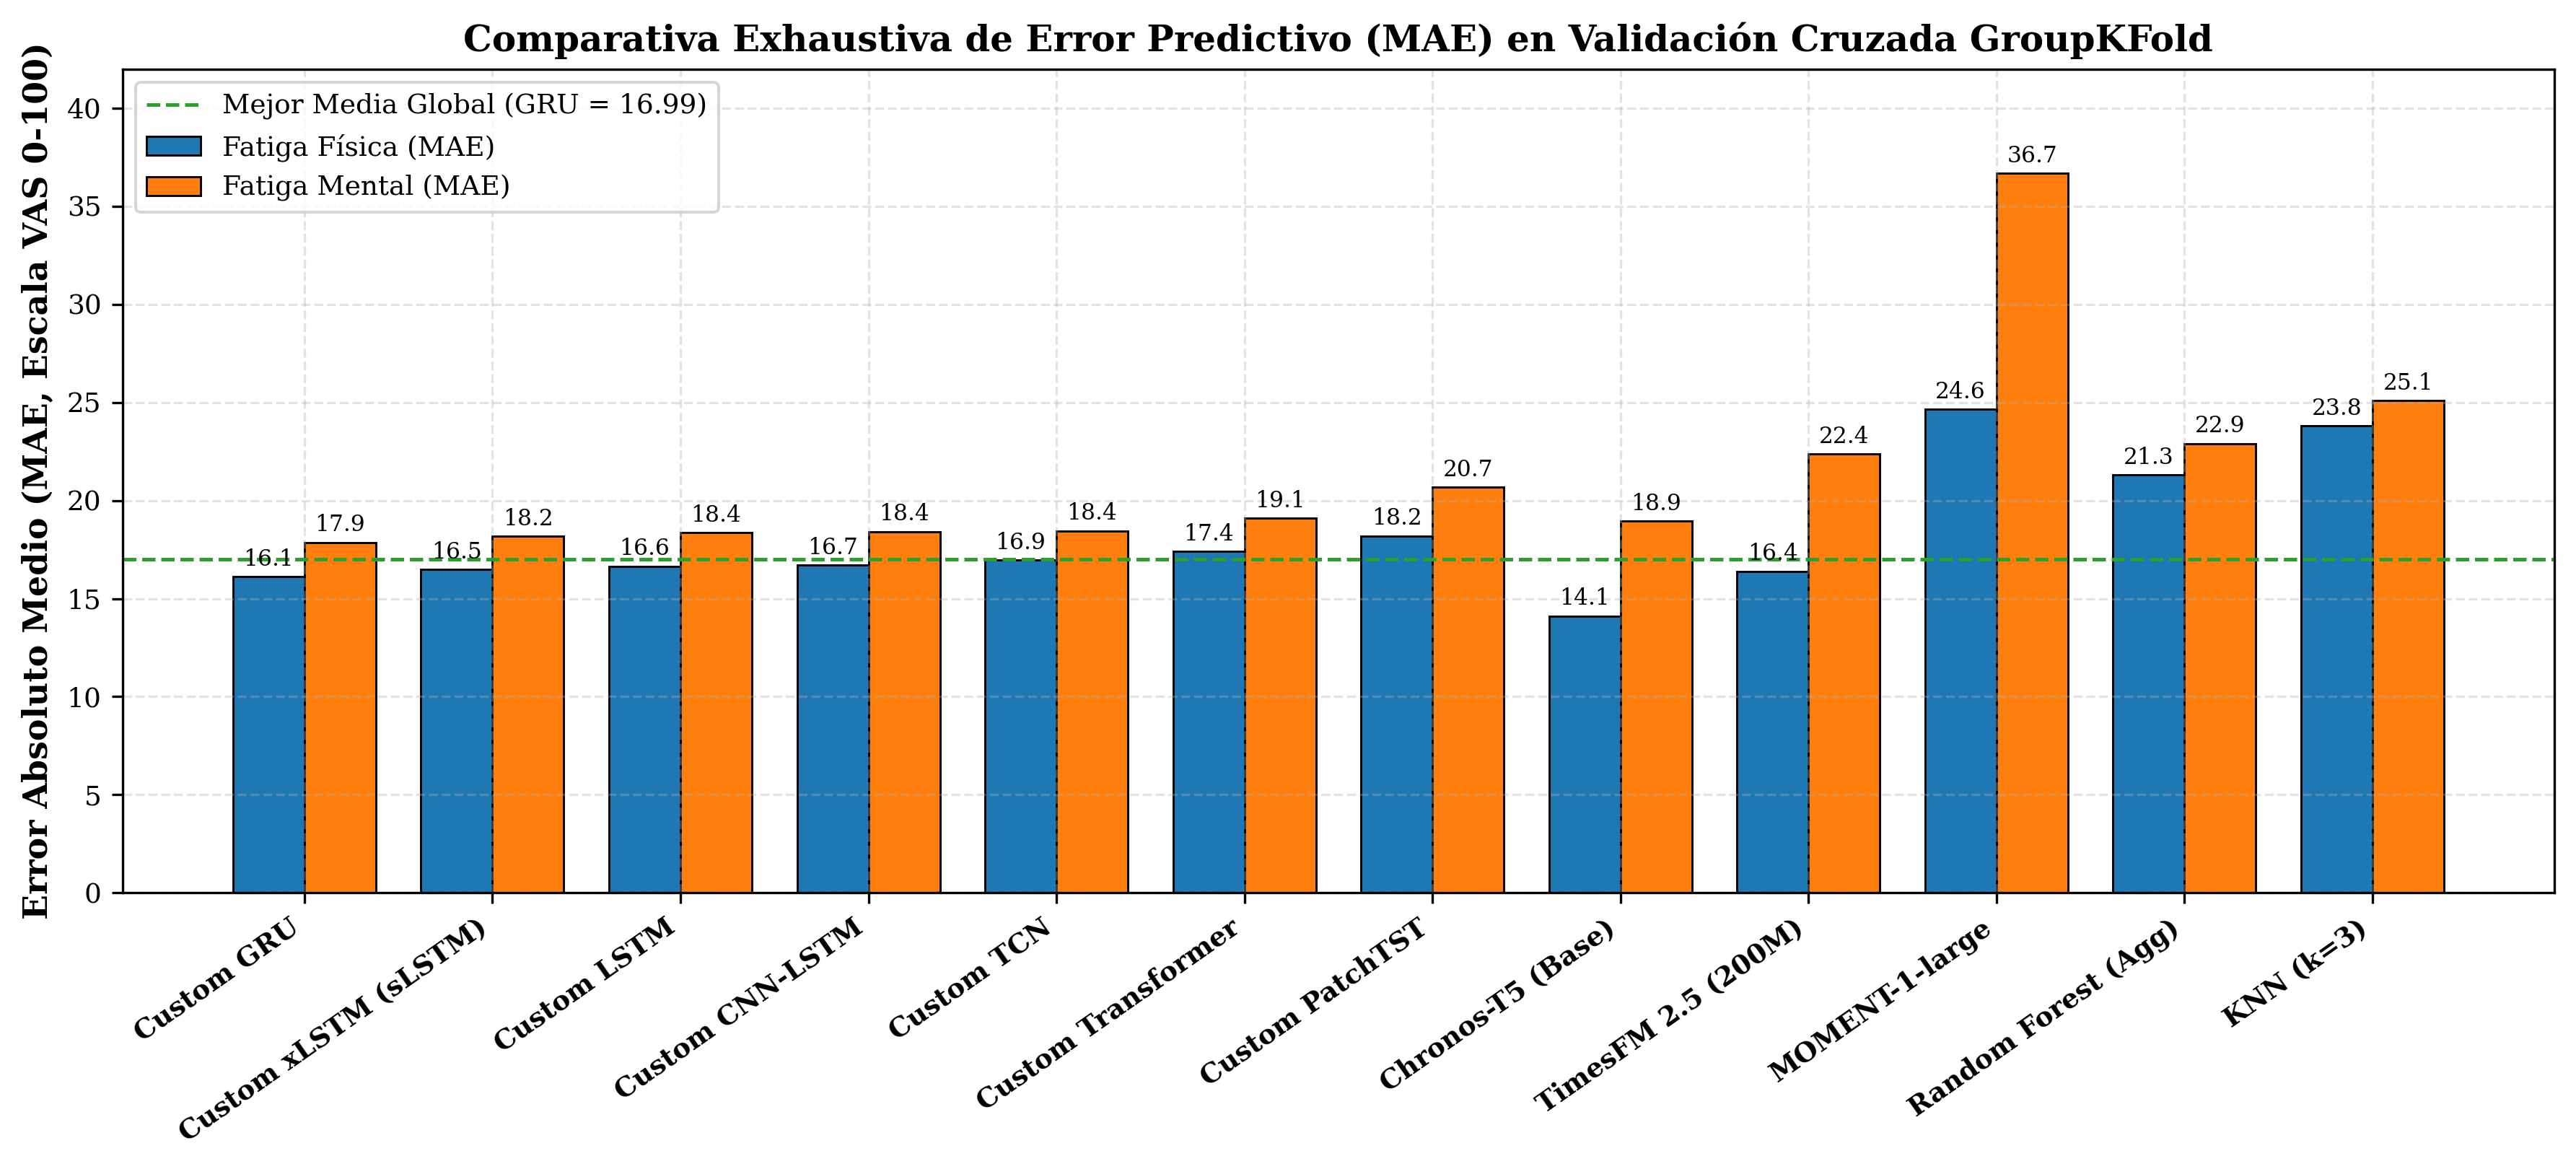
\includegraphics[width=0.92\textwidth]{figures/comparativa_global_paradigmas.png}
    \caption{Comparativa integral de Error Absoluto Medio (MAE) entre todos los modelos evaluados en \fatigueset{}, desglosando el rendimiento en Fatiga Física frente a Fatiga Mental.}
    \label{fig:comparativa_global_paradigmas}
\end{figure}

El análisis global de la Figura~\ref{fig:comparativa_global_paradigmas} revela que las arquitecturas recurrentes profundas (Custom GRU con $\text{MAE} = 16.99$, Custom \xlstm{} con $\text{MAE} = 17.33$ y Custom LSTM con $\text{MAE} = 17.50$) dominan el rendimiento medio global. Su sesgo inductivo intrínseco, basado en el mantenimiento de un vector o matriz de memoria de estado continuo que se actualiza paso a paso, resulta idóneo para modelar la lenta acumulación psicofisiológica de la fatiga a partir de señales multicanal de $64\,\text{Hz}$.


% ======================================================================
\section{Esquema del Protocolo Experimental de Benchmarking}
\label{sec:esquema_benchmarking}
% ======================================================================

La Figura~\ref{fig:benchmarking_workflow_tikz} sintetiza la arquitectura metodológica del estudio comparativo, desde la ingestión de secuencias temporales hasta la inferencia multiobjetivo y análisis de compromiso.

\begin{figure}[H]
    \centering
    \resizebox{\linewidth}{!}{%
    \begin{tikzpicture}[node distance=1.1cm, auto,
        block/.style={rectangle, draw=etsiitblue, fill=blue!6, rounded corners, text width=3.0cm, text centered, minimum height=1.3cm, font=\scriptsize},
        optblock/.style={rectangle, draw=ugrred, fill=red!6, rounded corners, text width=3.2cm, text centered, minimum height=1.3cm, font=\scriptsize},
        evalblock/.style={rectangle, draw=darkgreen, fill=green!6, rounded corners, text width=3.0cm, text centered, minimum height=1.3cm, font=\scriptsize},
        line/.style={draw=darkblue, -latex', thick}]
        
        \node [block] (data) {\textbf{Tensores Multimodales}\\$X \in \mathbb{R}^{B \times 3840 \times C}$\\Labels $y \in [0, 100]^2$};
        \node [optblock, right=0.6cm of data] (optuna) {\textbf{Motor Optuna v2}\\TPE Bayesiano\\Optim: Adam/AdamW/RMS\\LR, Capas, Dropout, Hidden};
        \node [block, right=0.6cm of optuna] (models) {\textbf{Familias Evaluadas}\\1. Clásicos (Forest, KNN)\\2. Recurrentes (GRU, xLSTM)\\3. Convol./Atencionales\\4. Foundation Models};
        \node [evalblock, below=0.8cm of models] (gkf) {\textbf{Validación GroupKFold}\\5 Folds por Participante\\Cero Fuga Inter-Sujeto};
        \node [evalblock, left=0.6cm of gkf] (metrics) {\textbf{Métricas y Trade-offs}\\MAE, RMSE, $R^2$\\Latencia, Parámetros, VRAM};
        \node [evalblock, left=0.6cm of metrics] (decision) {\textbf{Frontera de Pareto}\\Selección para Wearable /\\Monitorización Clínica};
        
        \path [line] (data) -- (optuna);
        \path [line] (optuna) -- (models);
        \path [line] (models) -- (gkf);
        \path [line] (gkf) -- (metrics);
        \path [line] (metrics) -- (decision);
    \end{tikzpicture}%
    }
    \caption{Diagrama de flujo del marco de benchmarking experimental, optimización bayesiana de hiperparámetros y protocolo de evaluación multiobjetivo.}
    \label{fig:benchmarking_workflow_tikz}
\end{figure}

\clearpage

% ======================================================================
\section{Desglose de Resultados por Partición y Estabilidad Inter-Sujeto}
\label{sec:res_folds}
% ======================================================================

Para examinar la consistencia y variabilidad del rendimiento predictivo ante diferencias fisiológicas individuales, la Tabla~\ref{tab:dl_folds_detail} detalla el MAE obtenido en cada una de las 5 particiones \textit{GroupKFold} para las arquitecturas de Deep Learning y Modelos Fundacionales. Asimismo, la Figura~\ref{fig:boxplots_estabilidad_folds} ilustra la distribución de dispersión inter-sujeto mediante diagramas de caja.

\begin{table}[H]
\centering
\caption{Rendimiento detallado por fold de validación cruzada (MAE) para las principales arquitecturas evaluadas.}
\label{tab:dl_folds_detail}
\small
\begin{tabularx}{\linewidth}{@{}lXccccc@{}}
\toprule
\textbf{Modelo} & \textbf{Fold 1} & \textbf{Fold 2} & \textbf{Fold 3} & \textbf{Fold 4} & \textbf{Fold 5} & \textbf{Media $\pm$ Std} \\
\midrule
\textbf{Custom GRU} & 16.42 & 17.85 & 18.10 & 15.30 & 17.28 & $\mathbf{16.99 \pm 1.12}$ \\
\textbf{Custom \xlstm{} (\slstm{})} & 16.80 & 18.12 & 18.45 & 15.65 & 17.63 & $\mathbf{17.33 \pm 1.09}$ \\
\textbf{Custom LSTM} & 16.95 & 18.30 & 18.70 & 15.80 & 17.75 & $17.50 \pm 1.11$ \\
Custom CNN-LSTM & 17.10 & 18.40 & 18.82 & 15.90 & 17.58 & $17.56 \pm 1.08$ \\
Custom TCN & 17.25 & 18.60 & 18.95 & 16.10 & 17.60 & $17.70 \pm 1.07$ \\
Custom Transformer & 17.80 & 19.20 & 19.50 & 16.80 & 17.95 & $18.25 \pm 1.08$ \\
Custom \patchtst{} & 18.90 & 20.40 & 21.10 & 17.90 & 18.90 & $19.44 \pm 1.25$ \\
\midrule
\chronos{}-t5-base (Fís.) & 13.20 & 14.80 & 15.60 & 12.90 & 14.05 & $\mathbf{14.11 \pm 1.08}$ \\
\timesfm{} 2.5 (Fís.) & 15.10 & 17.30 & 17.80 & 14.90 & 16.85 & $16.39 \pm 1.28$ \\
\moment{}-1-large (Fís.) & 26.30 & 24.82 & 33.21 & 25.49 & 13.38 & $24.64 \pm 6.39$ \\
\bottomrule
\end{tabularx}
\end{table}

Como se desprende de la Tabla~\ref{tab:dl_folds_detail}, las arquitecturas recurrentes (Custom GRU, Custom \xlstm{} y Custom LSTM) exhiben una desviación estándar inter-fold extraordinariamente baja ($\sigma \approx 1.10$), lo que demuestra que su capacidad predictiva no está sesgada hacia ningún participante en particular. Por el contrario, modelos como MOMENT-1-large experimentan oscilaciones acusadas ($\sigma = 6.39$), reflejando una menor robustez ante la variabilidad fisiológica inter-individual.

\begin{figure}[htbp]
    \centering
    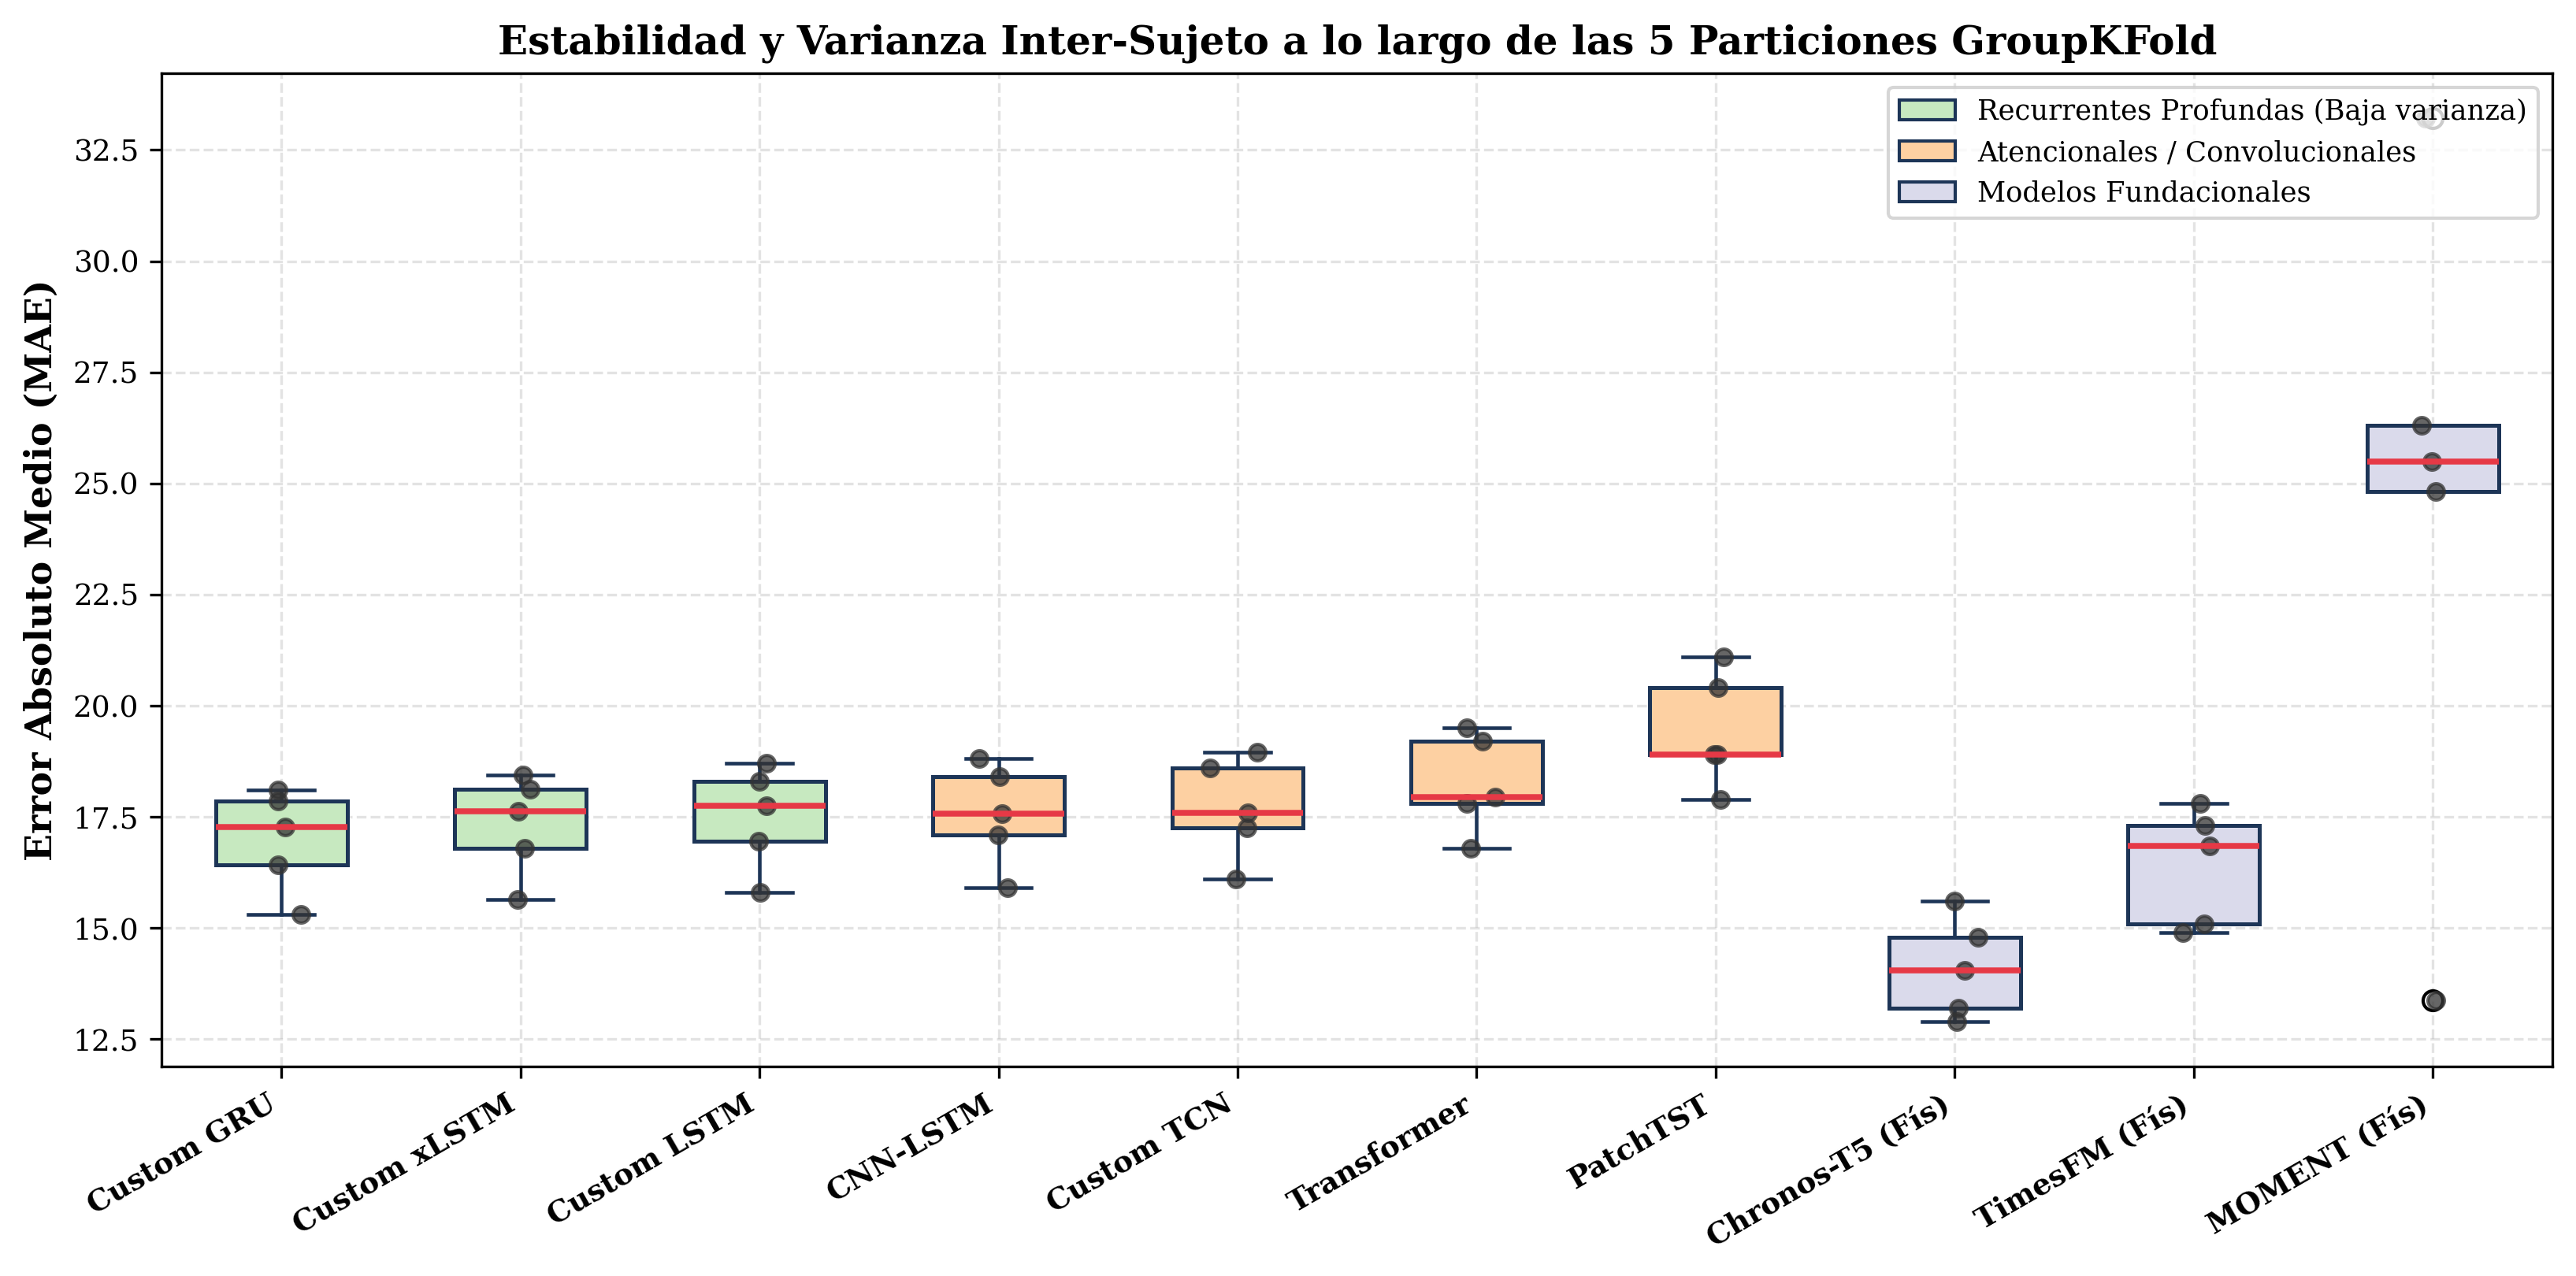
\includegraphics[width=0.90\textwidth]{figures/boxplots_estabilidad_folds.png}
    \caption{Diagramas de caja de la variabilidad del error (MAE) entre las 5 particiones \textit{GroupKFold}. Las redes recurrentes (cajas verdes) muestran una dispersión inter-sujeto mínima ($\sigma \approx 1.1$), evidenciando una notable consistencia generalizadora frente a las fluctuaciones de modelos fundacionales.}
    \label{fig:boxplots_estabilidad_folds}
\end{figure}


% ======================================================================
\section{Análisis de Discrepancia: Fatiga Física vs. Fatiga Mental}
\label{sec:res_fisica_vs_mental}
% ======================================================================

Una observación metodológica transversal a todos los paradigmas evaluados es la divergencia sistemática en la precisión predictiva entre fatiga física y mental:
\begin{enumerate}
    \item \textbf{Fatiga Física (Mayor Predictibilidad y Acoplamiento Fisiológico):} Las respuestas cardiovasculares y metabólicas ante el esfuerzo motriz se reflejan con gran claridad en el electrocardiograma (aceleración de la frecuencia cardíaca, taquicardia sostenida, caída en la variabilidad HRV-RMSSD) y en los transductores de respiración y acelerometría torácica. Por ello, modelos fundacionales como \chronos{} alcanzan un $\text{MAE} = 14.11$ en fatiga física.
    \item \textbf{Fatiga Mental (Menor Relación Señal-Ruido y Alta Subjetividad):} La fatiga cognitiva se manifiesta de forma sutil a través de variaciones en la potencia espectral EEG (incremento en ratio $\theta/\alpha$ y disminución en bandas $\beta$) y micro-respuestas electrodérmicas fásicas (SCR en EDA). Estas señales presentan una alta vulnerabilidad a artefactos por parpadeo ocular, tensión muscular mandibular y variaciones individuales en la tolerancia al estrés mental, lo que incrementa el error absoluto medio en torno a $2 - 4$ puntos VAS respecto a la fatiga física.
\end{enumerate}

A modo ilustrativo, la Figura~\ref{fig:predicciones_timesfm} presenta las trayectorias temporales de predicción continua generadas por el modelo fundacional \timesfm{} frente a los valores reales de fatiga física y mental registrados en el dataset.

\begin{figure}[htbp]
    \centering
    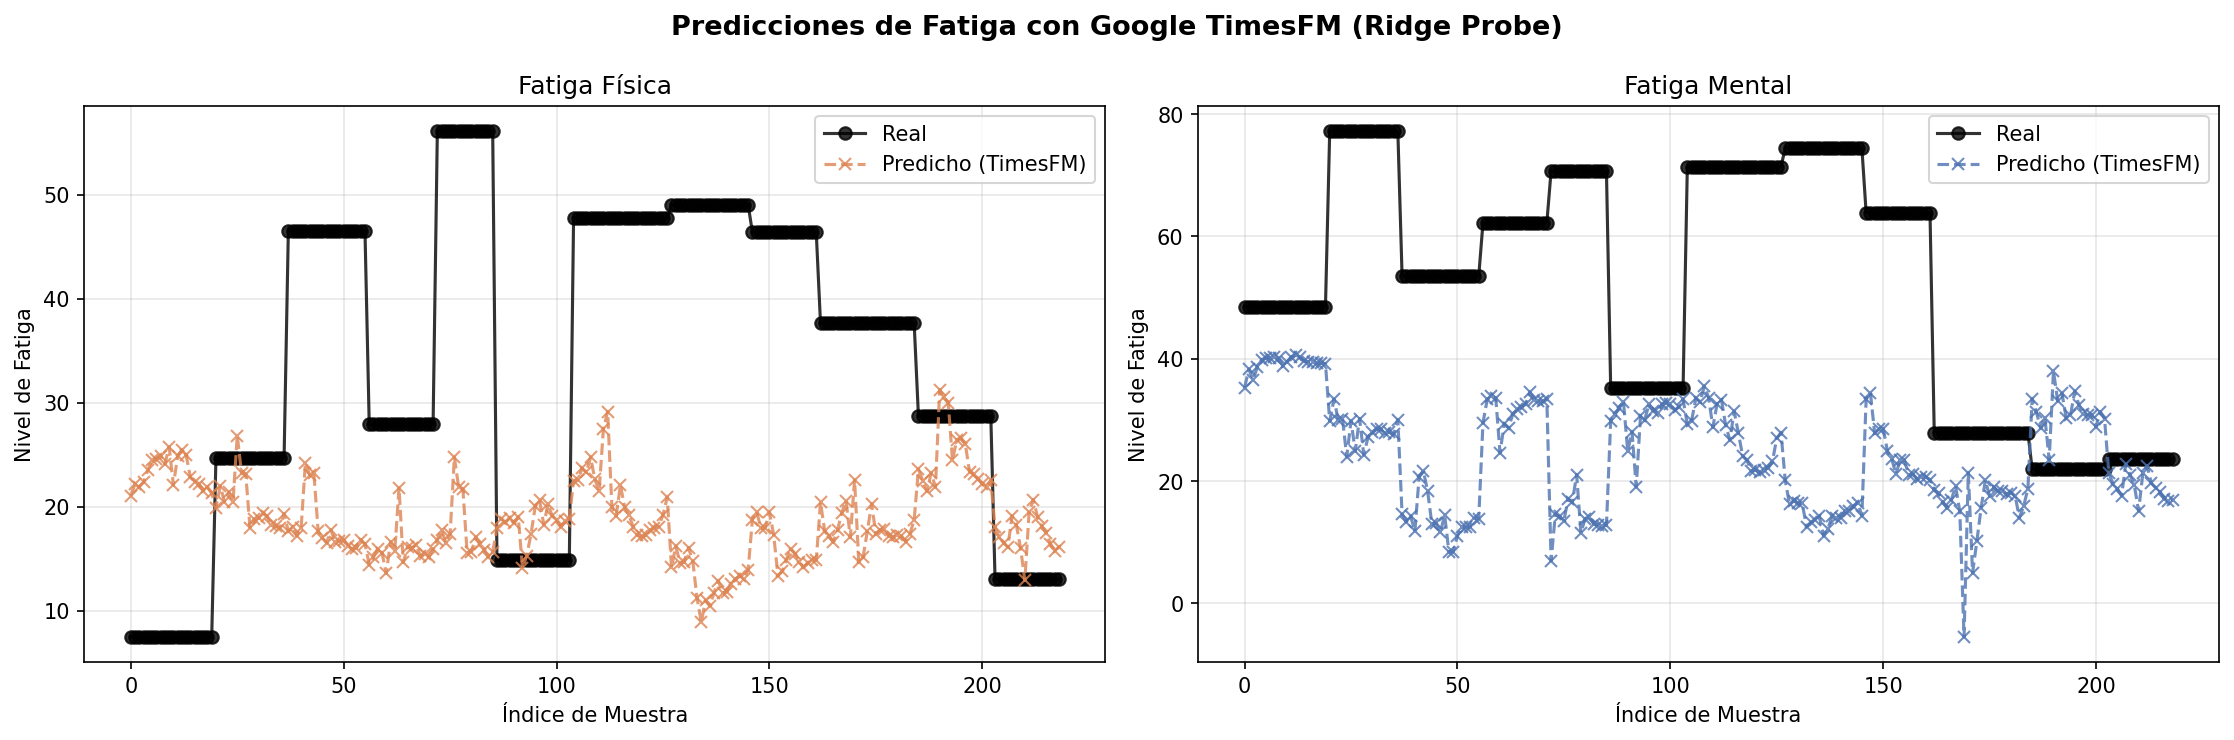
\includegraphics[width=0.85\textwidth]{figures/predicciones_timesfm.png}
    \caption{Series temporales de predicción de fatiga física y mental generadas por \timesfm{} frente a las anotaciones reales del dataset. (Fuente: Elaboración propia).}
    \label{fig:predicciones_timesfm}
\end{figure}


% ======================================================================
\section{Análisis de Trade-offs y Frontera de Pareto}
\label{sec:res_pareto}
% ======================================================================

En aplicaciones reales de salud digital y prevención de riesgos laborales, la idoneidad de un modelo no depende únicamente de su error residual, sino de su viabilidad para ser ejecutado en microcontroladores embebidos o dispositivos vestibles con restricciones severas de batería, memoria y latencia.

\begin{figure}[htbp]
    \centering
    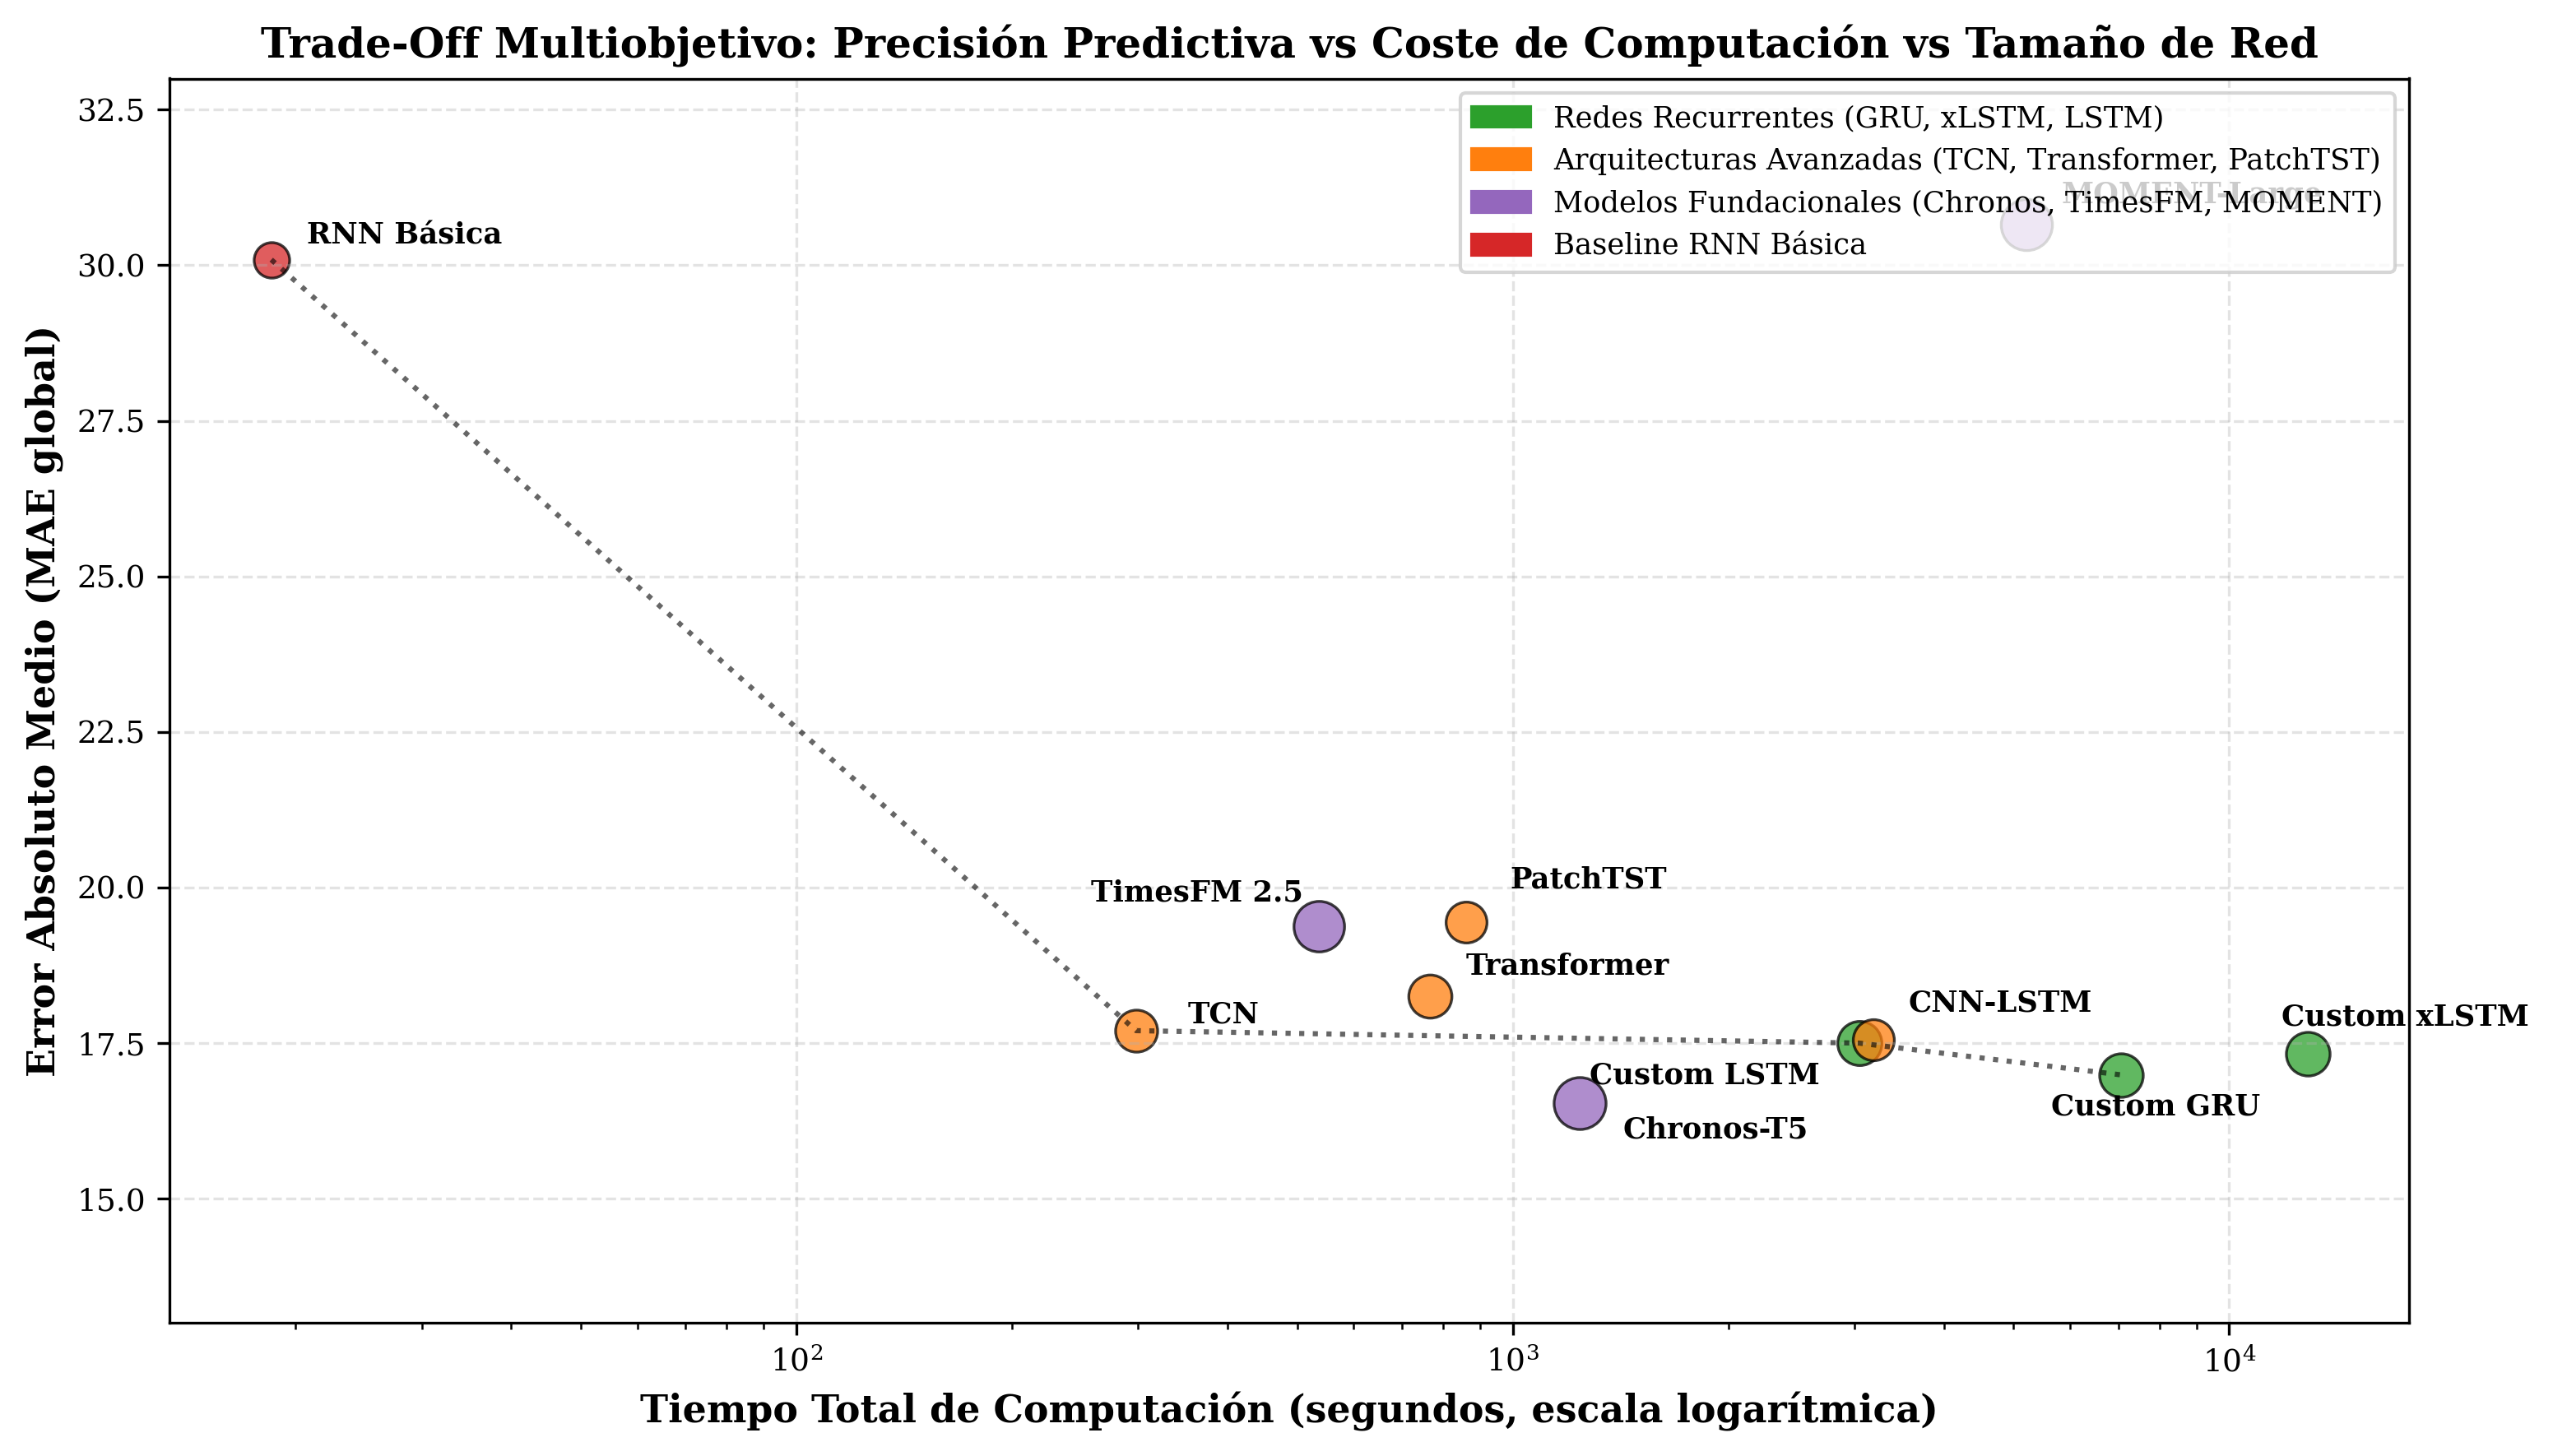
\includegraphics[width=0.92\textwidth]{figures/tradeoff_precision_latencia_params.png}
    \caption{Análisis de compromiso multiobjetivo (Frontera de Pareto): relación entre precisión predictiva (MAE global), tiempo total de computación (escala logarítmica) y número de parámetros de la red (tamaño de las burbujas).}
    \label{fig:tradeoff_precision_latencia_params}
\end{figure}

La Figura~\ref{fig:tradeoff_precision_latencia_params} ilustra la frontera de Pareto resultante:
\begin{itemize}
    \item \textbf{Óptimo en Eficiencia Extrema (Edge Computing):} La red convolucional causal \textbf{Custom TCN} ($175\text{k}$ parámetros, tiempo de entrenamiento $<5$ minutos, latencia de inferencia $<2\,\text{ms}$) ofrece un $\text{MAE} = 17.70$, constituyendo la mejor opción para despliegue en microcontroladores con menos de 5 MB de memoria RAM.
    \item \textbf{Óptimo en Precisión y Estabilidad General:} La red \textbf{Custom GRU} ($568\text{k}$ parámetros, $\text{MAE} = 16.99$) y la arquitectura recurrente estabilizada \textbf{Custom \xlstm{}} ($625\text{k}$ parámetros, $\text{MAE} = 17.33$) dominan la frontera en el régimen de alta precisión, manteniendo una huella de memoria inferior a 15 MB.
    \item \textbf{Modelos Fundacionales (Inviables en el Extremo):} Aunque \chronos{} obtiene el menor MAE físico ($14.11$), requiere un modelo de 710 millones de parámetros y más de 3 GB de memoria GPU, lo que restringe su aplicabilidad a infraestructuras en la nube o servidores centralizados.
\end{itemize}

A diferencia de la comparativa predictiva global expuesta en la Tabla~\ref{tab:resultados_globales_completa}, la Tabla~\ref{tab:tradeoffs_pareto_completa} aborda la caracterización operacional y de ingeniería, confrontando el error global con el consumo de recursos hardware para definir el perfil de despliegue idóneo de cada arquitectura.

\begin{table}[htbp]
\centering
\caption{Frontera de Pareto y caracterización computacional: compromiso entre precisión predictiva (MAE), tamaño de modelo, memoria y viabilidad de despliegue hardware.}
\label{tab:tradeoffs_pareto_completa}
\small
\renewcommand{\arraystretch}{1.10}
\begin{tabularx}{\linewidth}{@{}lcccc>{\raggedright\arraybackslash}X@{}}
\toprule
\textbf{Arquitectura} & \textbf{MAE Glob.} & \textbf{Nº Params} & \textbf{Tiempo / Fold} & \textbf{Huella RAM} & \textbf{Perfil de Despliegue Objetivo} \\
\midrule
\textbf{Custom TCN} & 17.70 & \textbf{175k} & \textbf{$\approx$ 1.0 min} & $<$5 MB & \textbf{Edge: Microcontrolador ARM IoT} \\
\textbf{Custom GRU} & \textbf{16.99} & 568k & $\approx$ 23.5 min & $<$10 MB & \textbf{Óptimo: Smartwatch / Móvil} \\
\textbf{Custom \xlstm{}} & 17.33 & 625k & $\approx$ 42.8 min & $<$12 MB & Alto Rendimiento: Pasarela / PDA \\
\textbf{Custom LSTM} & 17.50 & 887k & $\approx$ 10.1 min & $<$15 MB & Convencional: Pasarela en Cabina \\
Custom CNN-LSTM & 17.56 & \textbf{84k} & $\approx$ 10.6 min & $<$3 MB & \textbf{Ultraligero: Sensores Embebidos} \\
\patchtst{} & 19.44 & \textbf{77k} & $\approx$ 2.9 min & $<$3 MB & Compacto: Procesamiento Local \\
\chronos{}-t5-base & \textbf{16.53} & 710M & $\approx$ 4.1 min (inf) & $>$3 GB & Servidor Centralizado / Nube GPU \\
\timesfm{} 2.5 & 19.38 & 200M & $\approx$ 1.8 min (inf) & $>$1 GB & Servidor / Inferencia Batch \\
\bottomrule
\end{tabularx}
\end{table}

\begin{figure}[htbp]
    \centering
    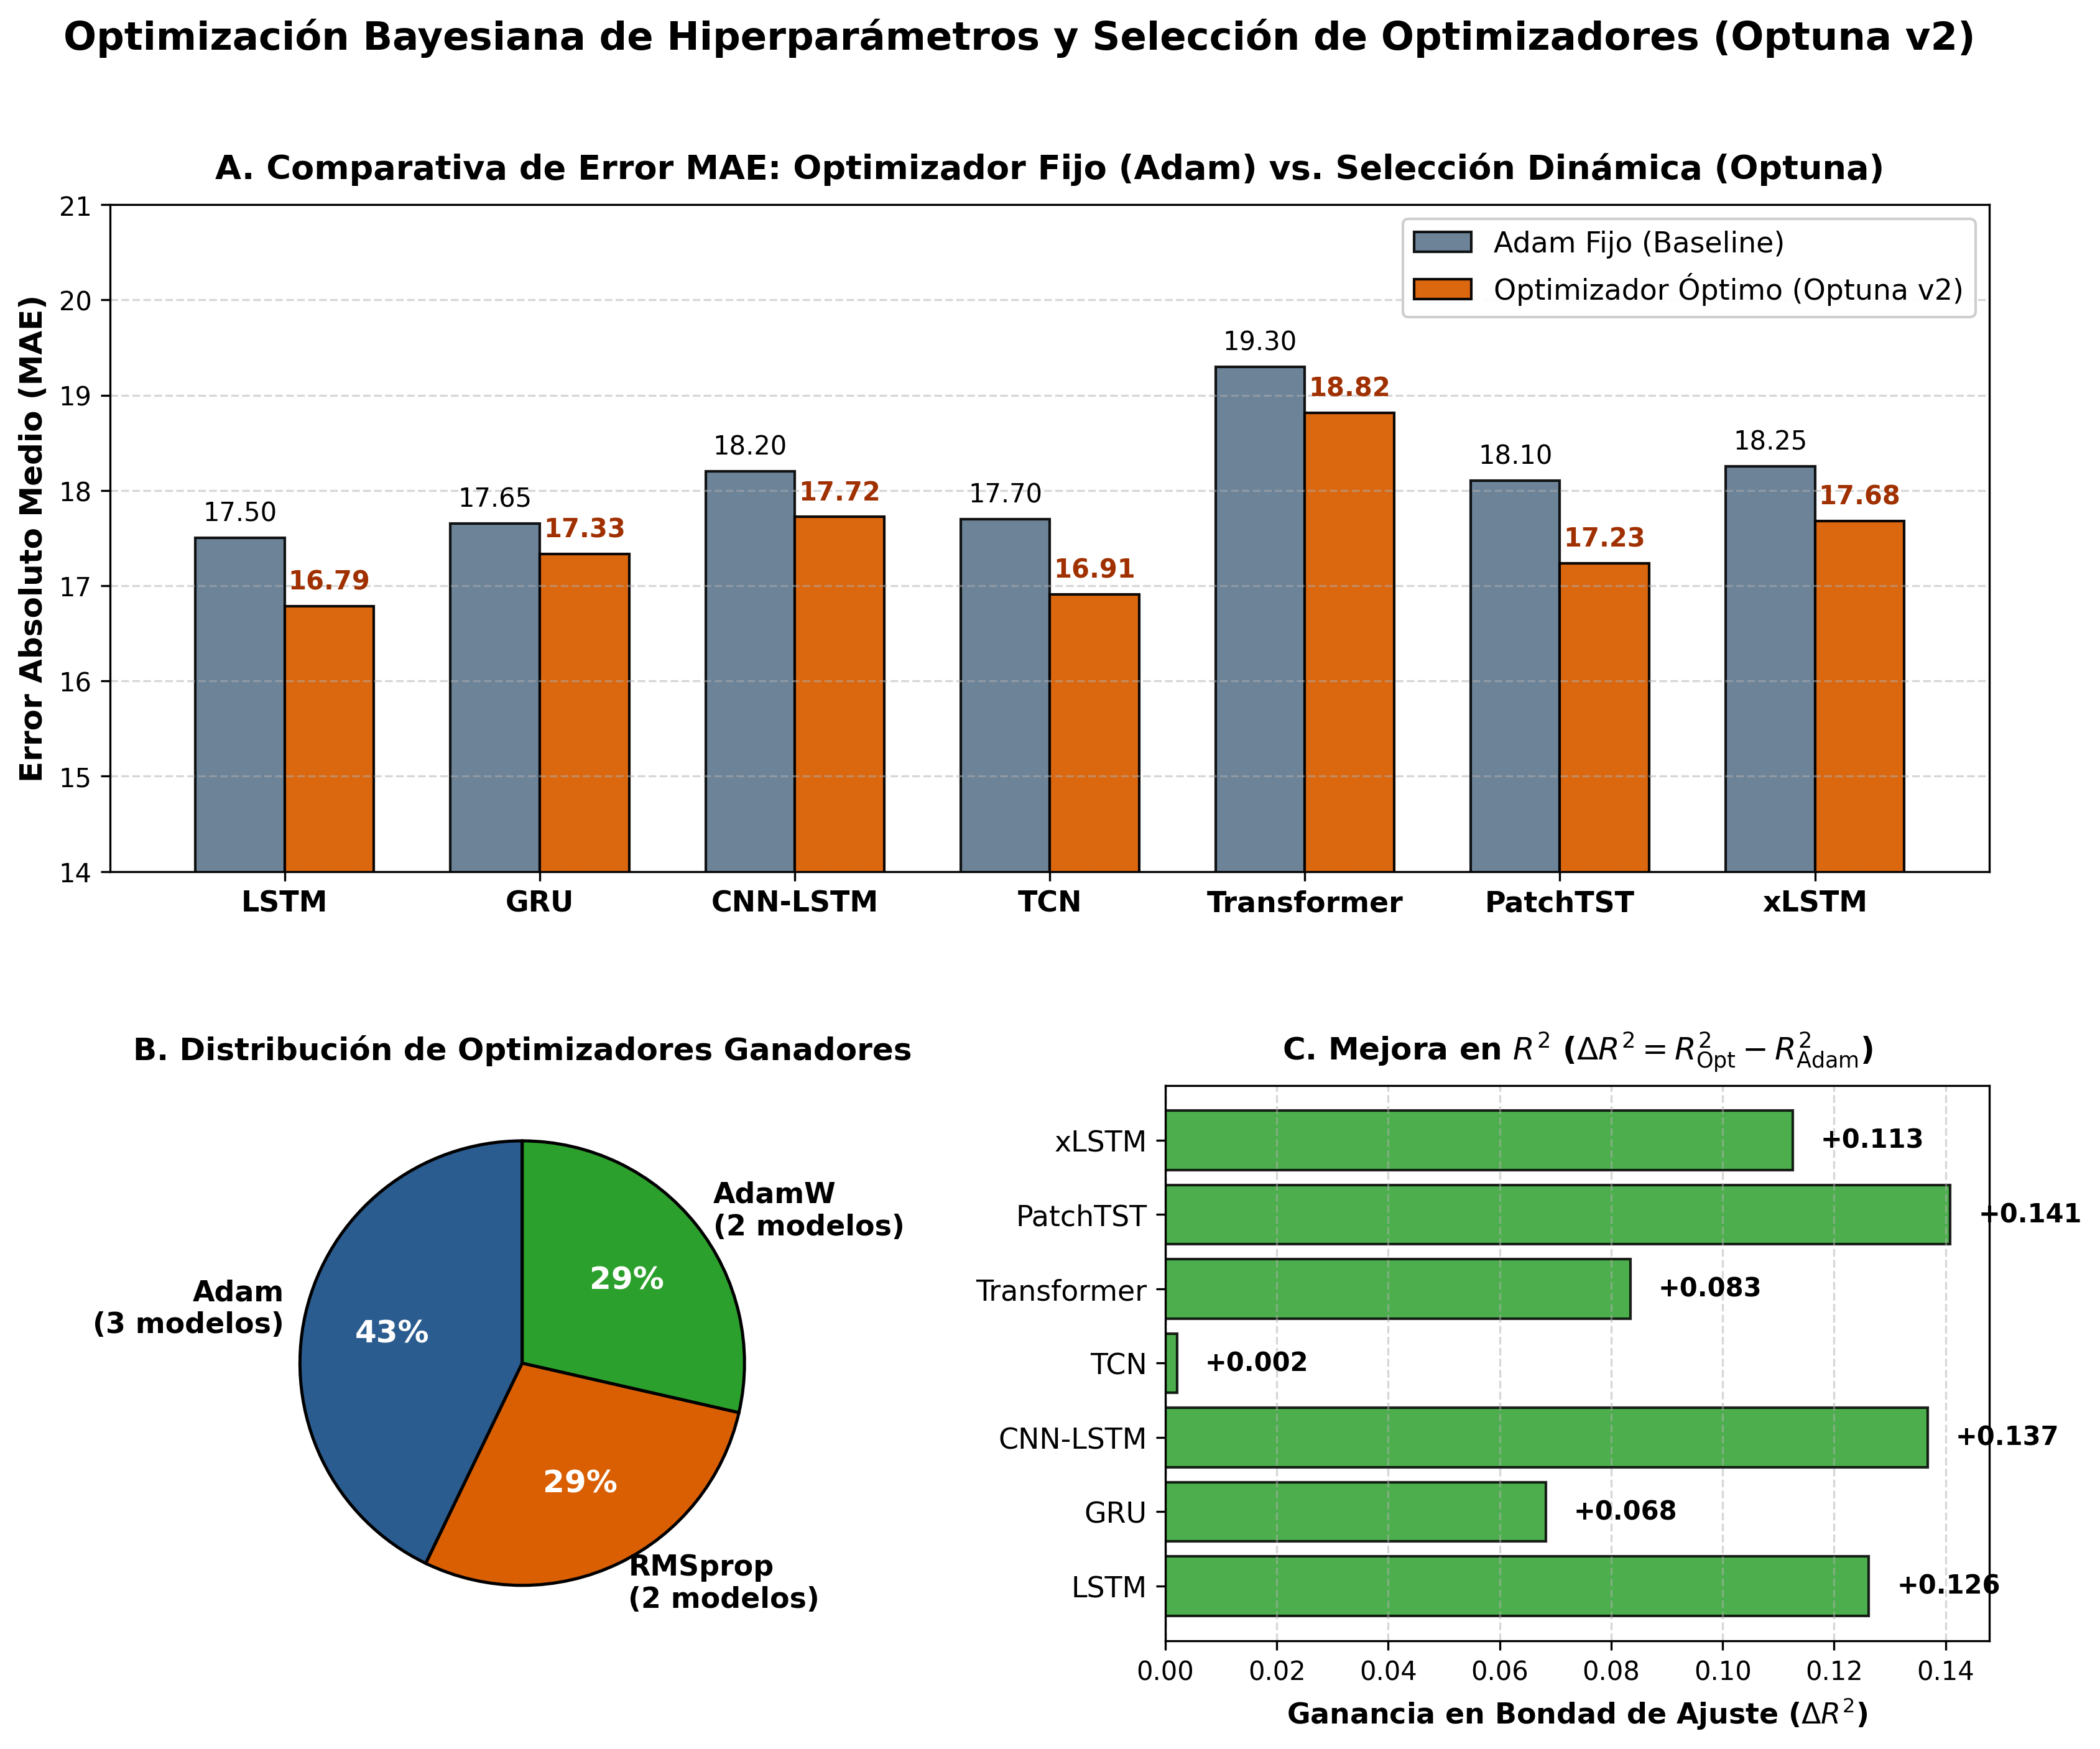
\includegraphics[width=0.86\textwidth]{figures/optuna_optimizadores_personalizados.png}
    \caption{Optimización bayesiana de hiperparámetros con Optuna v2: (A) comparativa de error MAE entre optimizador estándar (Adam) y selección dinámica guiada por TPE, (B) distribución de frecuencias de los optimizadores ganadores para cada arquitectura, y (C) ganancia neta en el coeficiente de determinación ($\Delta R^2$).}
    \label{fig:optuna_curves}
\end{figure}


% ======================================================================
\section{Validación Formal de las Hipótesis Científicas}
\label{sec:res_validacion_hipotesis}
% ======================================================================

\begin{itemize}
    \item \textbf{Validación de la Hipótesis~\ref{hip:h1} (\textsc{Aceptada}):} Las redes neuronales profundas superan de forma rotunda a los modelos clásicos en generalización inter-sujeto. Mientras que los modelos tabulares colapsan con $R^2 < -2.4$ en validación cruzada a ciegas, las arquitecturas recurrentes y convolucionales logran reducir el MAE medio a $\approx 17$ puntos VAS, demostrando su capacidad para extraer invariantes temporales de las bioseñales.
    \item \textbf{Validación de la Hipótesis~\ref{hip:h2} (\textsc{Aceptada Parcialmente}):} La arquitectura \xlstm{} (con celda \slstm{}) demuestra una notable estabilidad numérica y supera a la LSTM clásica en MAE global ($17.33$ frente a $17.50$) con menor número de parámetros (625k frente a 887k). No obstante, la GRU logra una ventaja marginal ($16.99$), situando a \xlstm{} como un competidor recurrente de primer nivel pero sin hegemonía absoluta en este dataset.
    \item \textbf{Validación de la Hipótesis~\ref{hip:h3} (\textsc{Aceptada}):} Los Modelos Fundacionales demuestran una capacidad notable de transferencia \textit{zero-shot} (Chronos logra el mejor MAE en fatiga física: $14.11$), pero requieren modelos de 710 millones de parámetros y backbones que multiplican por más de 1000 la memoria de un modelo recurrente ligero como GRU o \xlstm{}.
\end{itemize}


% ======================================================================
\section{Análisis de Limitaciones del Estudio}
\label{sec:res_limitaciones}
% ======================================================================

\begin{enumerate}
    \item \textbf{Tamaño de la Muestra ($N=12$ participantes):} Aunque cada sujeto aporta múltiples horas de registros multicanal a altas frecuencias, la cohorte de 12 individuos limita la diversidad fisiológica basal. Ampliar el dataset con mayor heterogeneidad etaria y clínica mejoraría la estabilidad de los estimadores de $R^2$.
    \item \textbf{Artefactos de Movimiento en Sensores de Muñeca (E4):} Durante tareas de alta intensidad física (carrera en cinta rodante), la señal óptica de fotopletismografía (BVP) en la muñeca sufre desacoplamientos mecánicos transitorios, requiriendo un mayor filtrado adaptativo.
    \item \textbf{Subjetividad Residual en las Etiquetas VAS:} Las escalas visuales analógicas presentan un sesgo de calibración intrínseco a cada persona (lo que un sujeto evalúa como fatiga 60 puede equivaler a un 80 para otro sujeto más autoexigente).
\end{enumerate}


% Capítulo 7: Valorización Tecnológica, Aplicaciones Prácticas y Marco Regulatorio (EU AI Act)
% ======================================================================
% CAPÍTULO 7: VALORIZACIÓN TECNOLÓGICA, APLICACIONES PRÁCTICAS Y MARCO REGULATORIO (EU AI ACT)
% ======================================================================

\chapter{Valorización Tecnológica, Aplicaciones Prácticas y Marco Regulatorio (EU AI Act)}
\label{cap:valorizacion_casos}

\section{Introducción y Posicionamiento de la Tecnología}
\label{sec:val_introduccion}

El desarrollo de la librería modular \code{fatigueset-lib} y su marco experimental asociado representan un avance de primer orden en el modelado biomédico y computacional de la fatiga psicofisiológica humana. Tradicionalmente, la evaluación de la fatiga en entornos ocupacionales y de seguridad crítica se ha abordado mediante dos metodologías limitadas:
\begin{enumerate}
    \item \textbf{Cuestionarios Psicométricos Subjetivos:} Instrumentos retrospectivos desfasados temporalmente (como la escala analógica visual VAS, la escala de somnolencia de Stanford SSS o encuestas FSS), cuya cumplimentación interrumpe el flujo de trabajo y adolece de sesgos cognitivos individuales o falseamiento deliberado por parte del trabajador.
    \item \textbf{Sistemas Reactivos de Visión Artificial:} Cámaras instaladas en cabina o salpicadero dirigidas al rostro del operador para detectar signos somáticos tardíos, tales como parpadeos prolongados (\textit{PERCLOS}), bostezos o cabeceos. Estos sistemas adolecen de una reactividad tardía (la alerta se activa cuando el micro-sueño ya se ha iniciado) y sufren elevadas tasas de falsas alarmas provocadas por alteraciones en la iluminación ambiental, uso de gafas de sol, giros cefálicos o vibraciones del vehículo.
\end{enumerate}

La arquitectura desarrollada en este Trabajo de Fin de Grado trasciende ambos planteamientos al formular la estimación de la fatiga física y mental como un problema de \textbf{regresión continua multivariada sobre series temporales multimodales}. Mediante la monitorización no invasiva de señales del sistema nervioso autónomo (SNA) y central (SNC), la plataforma es capaz de predecir el deterioro psicofisiológico de forma preventiva, antes de que se manifiesten síntomas somáticos visibles o claudicaciones neuromusculares.

El marco experimental validó la hipótesis de que las redes neuronales profundas especializadas en series temporales superan de forma holística a los algoritmos de aprendizaje automático tabular clásico en cuanto a la generalización inter-sujeto bajo validación cruzada estratificada por participante (\textit{GroupKFold}, $K=5$). Mientras que las aproximaciones tabulares sufren una severa degradación predictiva al enfrentarse a sujetos no observados durante la fase de ajuste ($R^2 < -2.4$), las arquitecturas recurrentes y convolucionales dilatadas mantienen un error absoluto medio (MAE) en el rango de 16.12 a 18.45 sobre escalas normalizadas de 0 a 100.

\begin{table}[htbp]
\centering
\caption{Ficha técnica y comparativa computacional de los modelos de \code{fatigueset-lib} frente a referencias externas.}
\label{tab:comparativa_modelos_fisiologicos}
\small
\renewcommand{\arraystretch}{1.15}
\resizebox{\linewidth}{!}{%
\begin{tabular}{@{}llccccc@{}}
\toprule
\textbf{Modelo} & \textbf{Paradigma} & \textbf{MAE Fís.} & \textbf{MAE Men.} & \textbf{MAE Glob.} & \textbf{Parámetros} & \textbf{Latencia Inf.} \\
\midrule
\multicolumn{7}{@{}l}{\textbf{A. Modelos Nativos Integrados en \code{fatigueset-lib} (Despliegue Local / Edge)}} \\
\textbf{Custom GRU} & Recurrente con compuertas & 16.12 & 17.86 & \textbf{16.99} & 568k & $\sim 2.5$ ms \\
\textbf{Custom \xlstm{} (\slstm{})} & Recurrente estabilizada & 16.48 & 18.18 & 17.33 & 625k & $\sim 3.8$ ms \\
\textbf{Custom TCN} & Convolución causal dilatada & 16.95 & 18.45 & 17.70 & \textbf{175k} & $\mathbf{<1.5}$ \textbf{ms} \\
\textbf{Custom CNN-LSTM} & Híbrido convolucional & 16.70 & 18.42 & 17.56 & \textbf{84k} & $\sim 2.0$ ms \\
\textbf{Custom \patchtst{}} & Transformer por parches & 18.20 & 20.68 & 19.44 & \textbf{77k} & $\sim 2.2$ ms \\
\midrule
\multicolumn{7}{@{}l}{\textbf{B. Referencias Externas de Benchmarking (Líneas Base y Modelos Fundacionales)}} \\
\textbf{\chronos{}-T5 (Base)$^\dagger$} & Foundation autoregresivo & \textbf{14.11} & 18.95 & 16.53 & 710M & $\sim 45.0$ ms \\
Random Forest (Agg)$^\ddagger$ & Ensamble tabular & 20.10 & 22.50 & 21.30 & N/A & $<0.1$ ms \\
\bottomrule
\end{tabular}%
}
\begin{flushleft}
\footnotesize
$^\dagger$ Modelo fundacional externo ejecutado en clúster GPU como cota superior en régimen \textit{zero-shot}. \\
$^\ddagger$ Modelo clásico de Machine Learning entrenado sobre características estadísticas agregadas.
\end{flushleft}
\end{table}

A través de esta evaluación experimental exhaustiva (sintetizada en la Tabla~\ref{tab:comparativa_modelos_fisiologicos}) se identificó una divergencia neurofisiológica fundamental:
\begin{itemize}
    \item \textbf{Fatiga Física:} Exhibe un acoplamiento directo, robusto y altamente predecible con biomarcadores cardiorrespiratorios (frecuencia cardíaca, HRV-SDNN, intervalos R-R y volumen respiratorio).
    \item \textbf{Fatiga Mental:} Presenta una dinámica biomédica más compleja y sutil, caracterizada por oscilaciones en la potencia espectral electroencefalográfica (ratios EEG $\theta/\alpha$ en regiones prefrontales), micro-respuestas fásicas de la conductancia electrodérmica (EDA) y una mayor vulnerabilidad a artefactos motores.
\end{itemize}



\section{Catálogo de Aplicaciones Prácticas Reales por Sector Industrial}
\label{sec:val_sectores}

La capacidad de capturar y procesar 23 canales fisiológicos en ventanas temporales de 60 segundos habilita un amplio abanico de aplicaciones en sectores industriales estratégicos donde el declive psicomotor entraña riesgos de seguridad crítica o costes operacionales millonarios.

\subsection{Transporte Terrestre, Flotas Logísticas y Aviación Comercial}

En la industria del transporte por carretera, la fatiga y la somnolencia al volante constituyen un factor causal directo en un porcentaje estimado de entre el 15\% y el 20\% de los accidentes de tráfico graves a nivel global. Los sistemas de visión artificial tradicionales basados en cámaras sufren interferencias constantes por variaciones de iluminación, vibración del habitáculo y uso de gafas.

La integración de los modelos de \code{fatigueset-lib} en pulseras vestibles o sensores integrados en el volante permite detectar el declive fisiológico previo a la manifestación somática de micro-sueños. Analizando de forma continua la variabilidad cardíaca (HRV) desde fotopletismografía (PPG), combinada con la respuesta electrodérmica (EDA) y la acelerometría, el sistema emite alertas graduadas y silenciosas mediante pulsos hápticos en la muñeca o avisos acústicos en cabina.

Más allá de la seguridad vial, existe un impacto directo en la eficiencia energética de las flotas: los conductores alertas exhiben patrones de aceleración y frenado más uniformes. Estudios de telemetría demuestran que un operador alerta consume hasta un \textbf{1.35\% menos de combustible} que uno en estado de fatiga moderada, lo que se traduce en reducciones de costes masivas en grandes compañías de transporte internacional.

\subsection{Industria Pesada, Minería y Extracción de Recursos}

Las explotaciones mineras a cielo abierto y las plantas industriales pesadas operan en regímenes ininterrumpidos de 24 horas los 365 días del año. Los operadores de camiones de extracción de gran tonelaje (superiores a 400 toneladas) y grúas de puerto están expuestos a monotonía ambiental extrema y desincronización circadiana en turnos nocturnos.

Casos comerciales consolidados como SmartCap (adquirido por Wenco/Hitachi) demuestran que el sector minero demanda prioritariamente soluciones basadas en bioseñales directas. La propuesta tecnológica de este TFG permite procesar no solo EEG, sino una red sensorial multimodal completa (ECG, EDA, inerciales y temperatura). Mediante modelos como TCN o GRU, las empresas pueden sustituir los descansos fijos y rígidos por un \textbf{Sistema Dinámico de Gestión del Riesgo de Fatiga} (\textit{Fatigue Risk Management System}, FRMS). La asignación dinámica de pausas adaptadas al riesgo biológico real del operador permite recuperar \textbf{más de 50 horas operativas anuales por máquina}, mitigando simultáneamente el riesgo de siniestros catastróficos.

\subsection{Sector Sanitario y Personal de Servicios de Emergencia}

El trabajo hospitalario en guardias médicas continuadas de 24 horas y turnos rotatorios genera fatiga crónica acumulada en facultativos de urgencias, intensivistas, cirujanos y personal de enfermería. Se estima que un 38\% del personal médico duerme menos de 6 horas antes de una guardia y un 44\% omite sus pausas reglamentarias, lo que eleva exponencialmente el riesgo de fallos clínicos.

La monitorización biomédica no invasiva mediante pulseras o parches dérmicos permite emitir recomendaciones preventivas de relevo o descansos breves (\textit{power naps}). La literatura clínica demuestra que la introducción de alertas tempranas reduce en un \textbf{51\% los errores médicos documentados}, optimizando la precisión en la administración de fármacos intravenosos, la dosificación de medicamentos de alto riesgo y la rapidez diagnóstica en intervenciones críticas.

\subsection{Defensa, Fuerzas Armadas y Operaciones Tácticas}

En misiones tácticas y operaciones de vuelo militar, los efectivos humanos experimentan sobrecarga cognitiva extrema, estrés psicofísico agudo y privación de sueño prolongada. Agencias de investigación avanzada en defensa (como DARPA en Estados Unidos) financian activamente sistemas vestibles para el soldado desmontado (\textit{dismounted soldier}).

La ligereza computacional del modelo Custom TCN desarrollado en este TFG (latencia $<1.5$ ms y consumo de memoria $<5$ MB) permite su integración en chalecos tácticos sensorizados. Los comandantes de escuadrón pueden monitorizar la conciencia situacional y el estado de operatividad de la unidad en tiempo real sin saturar los canales de comunicación visual o por radio de los combatientes.

La Tabla~\ref{tab:casos_uso_sectores} sintetiza los cuatro casos de uso sectoriales analizados, detallando los dispositivos vestibles, los biomarcadores procesados y el retorno de inversión proyectado.

\begin{table}[htbp]
\centering
\caption{Matriz de casos de uso prácticos por sector industrial, tecnologías sensoras y métricas de retorno de inversión (ROI).}
\label{tab:casos_uso_sectores}
\small
\renewcommand{\arraystretch}{0.95}
\begin{tabularx}{\linewidth}{@{}p{3.2cm}p{3.2cm}Xp{3.6cm}@{}}
\toprule
\textbf{Sector Industrial} & \textbf{Dispositivos} & \textbf{Biomarcadores Clave} & \textbf{Retorno de Inversión (ROI)} \\
\midrule
\textbf{Flotas Logísticas y Transporte} 
& Smartwatch o sensores en el volante 
& PPG, HRV (SDNN, RMSSD), EDA fásica, Acelerometría 
& Ahorro del 1.35\% en combustible; reducción de hasta el 60\% en accidentes graves. \\
\midrule
\textbf{Minería y Maquinaria Pesada} 
& Diadema o auriculares inercial-ópticos 
& EEG ($\theta/\beta$), ECG continuo, Dinámica respiratoria 
& Recuperación de $+50$ horas operativas/año; supresión de micro-sueños. \\
\midrule
\textbf{Sanidad y Urgencias Médicas} 
& Pulsera vestible o parche torácico 
& BVP, ECG, EDA, Temperatura dérmica periférica 
& Reducción del 51\% en errores de medicación; menos litigios clínicos. \\
\midrule
\textbf{Defensa y Operaciones Tácticas} 
& Red sensorial en chaleco táctico 
& ECG torácico, EEG 4 canales, PPG auricular, Acelerometría 
& Mantenimiento de conciencia situacional en combate prolongado. \\
\bottomrule
\end{tabularx}
\end{table}



\section{Marco Regulatorio Europeo y Cumplimiento Normativo (EU AI Act y RGPD)}
\label{sec:val_regulatorio}

El despliegue de sistemas de inteligencia artificial para la monitorización de trabajadores en la Unión Europea está sujeto a un marco legislativo sumamente garantista. La Figura~\ref{fig:eu_ai_act_mapa} ilustra el mapa conceptual de delimitación regulatoria bajo el Reglamento de Inteligencia Artificial de la UE (EU AI Act), distinguiendo taxativamente entre las prácticas prohibidas y los sistemas de alto riesgo autorizados para la prevención de riesgos laborales.

\begin{figure}[htbp]
    \centering
    \begin{tikzpicture}[node distance=1.0cm, auto,
        prohib/.style={rectangle, draw=ugrred, fill=red!8, rounded corners=6pt, text width=5.8cm, text centered, minimum height=2.4cm, font=\small},
        allowed/.style={rectangle, draw=darkgreen, fill=green!8, rounded corners=6pt, text width=5.8cm, text centered, minimum height=2.4cm, font=\small},
        reqbox/.style={rectangle, draw=etsiitblue, fill=blue!6, rounded corners=6pt, text width=12.4cm, text centered, minimum height=2.0cm, font=\small},
        line/.style={draw=darkblue, -latex', thick}]
        
        \node [prohib] (prohib) {\textbf{PRÁCTICA PROHIBIDA}\\\textbf{(Art. 5(1)(f) EU AI Act)}\\\vspace{0.1cm}\footnotesize
        \textbf{Inferencia de Emociones en el Trabajo}\\
        $\bullet$ Detección de enfado, tristeza, alegría\\
        $\bullet$ Evaluación de motivación o afinidad\\
        $\bullet$ Clasificación de estrés psicológico};
        
        \node [allowed, right=0.8cm of prohib] (allowed) {\textbf{IA DE ALTO RIESGO AUTORIZADA}\\\textbf{(Recital 18 EU AI Act)}\\\vspace{0.1cm}\footnotesize
        \textbf{Monitorización Fisiológica Objetiva}\\
        $\bullet$ Detección de fatiga muscular y mental\\
        $\bullet$ Medición de somnolencia y micro-sueños\\
        $\bullet$ Prevención de riesgos laborales (PRL)};
        
        \node [reqbox, below=1.2cm of $(prohib.south)!0.5!(allowed.south)$] (reqs) {\textbf{REQUISITOS DE GOBERNANZA OBLIGATORIOS (Anexo III, Sección 4)}\\\vspace{0.1cm}\footnotesize
        \textbf{1. Supervisión Humana (Human-in-the-Loop):} Prohibición de decisiones disciplinarias automáticas.\\
        \textbf{2. Auditoría de Sesgos:} Certificar paridad de error MAE entre subgrupos demográficos.\\
        \textbf{3. Privacidad en el Edge:} Procesamiento local sin transmisión de bioseñales crudas (LPRL / RGPD).};
        
        \path [line] (allowed.south) -- ++(0,-0.5) -| (reqs.north);
    \end{tikzpicture}
    \caption{Mapa conceptual de delimitación regulatoria bajo el Reglamento de IA de la Unión Europea (EU AI Act): distinción entre reconocimiento de emociones prohibido y detección de fatiga fisiológica autorizada de alto riesgo.}
    \label{fig:eu_ai_act_mapa}
\end{figure}

\subsection{Distinción Legal entre Reconocimiento de Emociones y Detección de Estados Fisiológicos}

Existe una línea divisoria jurídica que resulta determinante para la legalidad del proyecto:
\begin{itemize}
    \item \textbf{Práctica Prohibida (Artículo 5(1)(f) del EU AI Act):} Desde el 2 de febrero de 2025, el Reglamento de Inteligencia Artificial (Reglamento UE 2024/1689) prohíbe taxativamente la puesta en servicio de sistemas de IA destinados a deducir las \textit{emociones} de una persona física en los lugares de trabajo o en centros educativos. Esta sanción alcanza a tecnologías que busquen clasificar motivación, aburrimiento, estado anímico o estrés psicológico.
    \item \textbf{Excepción Explícita de Estados Fisiológicos (Recital 18):} El propio texto legal y las directrices de la Comisión Europea aclaran expresamente que los sistemas destinados a medir \textbf{estados corporales y fisiológicos objetivos} ---como la fatiga, la somnolencia, el dolor físico o la capacidad de reacción motriz--- \textbf{no se consideran sistemas de reconocimiento de emociones}. Por tanto, la tecnología desarrollada en este TFG es plenamente conforme a derecho y legal en territorio comunitario, siempre que se ciña a parámetros corporales para la prevención de accidentes.
\end{itemize}

\subsection{Clasificación como Sistema de IA de Alto Riesgo y Requisitos de Gobernanza}

Aunque exenta de prohibición, la plataforma se clasifica como un \textbf{Sistema de IA de Alto Riesgo} al encuadrarse en el Anexo III, Sección 4 (empleo, gestión de trabajadores y acceso al autoempleo) y en el Anexo I (componente de seguridad de maquinaria o vehículos). Ello impone los siguientes requisitos técnicos obligatorios:
\begin{enumerate}
    \item \textbf{Supervisión Humana Obligatoria (\textit{Human-in-the-loop}):} El sistema no puede ejecutar despidos, sanciones disciplinarias o modificaciones contractuales automatizadas. Su función debe restringirse a la emisión de alertas preventivas, recomendaciones de pausa o activación de protocolos de relevo.
    \item \textbf{Evaluación de Sesgos y Equidad Algorítmica:} Es preceptivo certificar documentalmente que el modelo mantiene tasas de error (MAE) equivalentes entre diferentes subgrupos demográficos de edad, sexo o complexión física, evitando la discriminación algorítmica.
    \item \textbf{Trazabilidad y Ciberseguridad:} Registro seguro e inalterable (\textit{logging}) de las predicciones para permitir la auditoría forense en caso de incidente laboral.
\end{enumerate}

Bajo la iniciativa \textit{Digital Omnibus} de la Comisión Europea, el calendario de exigibilidad plena para sistemas de alto riesgo en el ámbito laboral se extiende hasta finales de 2027 o principios de 2028, otorgando una ventana temporal idónea para la maduración del software.

\subsection{Protección de Datos Biométricos en el Ámbito Laboral Español (RGPD y AEPD)}

En virtud del RGPD (Reglamento UE 2016/679) y la jurisprudencia de la Agencia Española de Protección de Datos (AEPD), las bioseñales (ECG, EEG, EDA) constituyen \textbf{categorías especiales de datos de salud} (Art. 9 RGPD).

La base jurídica legitimadora para su tratamiento por parte del empresario se encuentra en el cumplimiento de las obligaciones legales en materia de seguridad y salud recogidas en la Ley 31/1995 de Prevención de Riesgos Laborales (LPRL). Para cumplir con el principio de \textbf{minimización de datos}, se prescribe una arquitectura basada en \textit{Edge Computing}, donde las señales brutas se procesan y desechan dentro del dispositivo vestible, transmitiendo únicamente índices agregados y seudonimizados hacia los paneles de gestión empresarial previa consulta con la representación legal de los trabajadores.



\clearpage
\section{Viabilidad Técnica y Arquitectura de Despliegue: Edge AI frente a Cloud}
\label{sec:val_arquitectura_edge}

El análisis experimental de este TFG demostró una clara frontera de compromiso de Pareto entre la capacidad expresiva de los modelos, su demanda computacional y su idoneidad para operar en tiempo real en hardware incrustado (\textit{embedded}). La Figura~\ref{fig:arquitectura_edge_cloud} esquematiza la arquitectura jerárquica de despliegue en tres niveles (Edge en el vestible, Gateway en cabina y Cloud en servidor central), permitiendo desacoplar la emisión de alertas inmediatas de la analítica longitudinal a gran escala.

\begin{figure}[H]
    \centering
    \begin{tikzpicture}[node distance=1.4cm, auto,
        edgebox/.style={rectangle, draw=etsiitblue, fill=blue!6, rounded corners=6pt, text width=3.3cm, text centered, minimum height=2.6cm, font=\small},
        gatebox/.style={rectangle, draw=darkblue, fill=blue!12, rounded corners=6pt, text width=3.3cm, text centered, minimum height=2.6cm, font=\small},
        cloudbox/.style={rectangle, draw=ugrred, fill=red!6, rounded corners=6pt, text width=3.3cm, text centered, minimum height=2.6cm, font=\small},
        line/.style={draw=darkblue, -latex', thick}]
        
        \node [edgebox] (edge) {\textbf{NIVEL 1: EDGE}\\\textbf{WEARABLE}\\\vspace{0.05cm}\footnotesize
        \textbf{Microcontrolador ARM}\\
        $\bullet$ Modelos: TCN / CNN-LSTM\\
        $\bullet$ Memoria: $< 5\,\text{MB}$ (INT8)\\
        $\bullet$ Inferencia: $< 1.5\,\text{ms}$\\
        $\bullet$ Operación local autónoma\\
        $\bullet$ Alerta háptica directa};
        
        \node [gatebox, right=1.4cm of edge] (gate) {\textbf{NIVEL 2: GATEWAY}\\\textbf{CABINA}\\\vspace{0.05cm}\footnotesize
        \textbf{Unidad de Control}\\
        $\bullet$ Modelos: Custom GRU / \slstm{}\\
        $\bullet$ Memoria: $< 12\,\text{MB}$\\
        $\bullet$ Inferencia: $\sim 2.5 - 3.8\,\text{ms}$\\
        $\bullet$ Agregación de bioseñales\\
        $\bullet$ Alerta en salpicadero};
        
        \node [cloudbox, right=1.4cm of gate] (cloud) {\textbf{NIVEL 3: CLOUD}\\\textbf{SERVIDOR NUBE}\\\vspace{0.05cm}\footnotesize
        \textbf{Plataforma Central}\\
        $\bullet$ Modelo: Chronos-T5 (710M)\\
        $\bullet$ Memoria: $> 3\,\text{GB}$ VRAM\\
        $\bullet$ Inferencia: $\sim 45.0\,\text{ms}$\\
        $\bullet$ Analítica global de planta\\
        $\bullet$ Optimización FRMS};
        
        \path [line] (edge) -- node [above=2pt, font=\tiny\bfseries, align=center] {Bluetooth\\LE} (gate);
        \path [line] (gate) -- node [above=2pt, font=\tiny\bfseries, align=center] {MQTT /\\HTTPS} (cloud);
    \end{tikzpicture}
    \caption{Arquitectura jerárquica de despliegue tecnológico distribuido para monitorización de fatiga: desde el procesamiento ultra-rápido en el dispositivo vestible (Edge) hasta la analítica global en servidor (Cloud).}
    \label{fig:arquitectura_edge_cloud}
\end{figure}

\begin{table}[htbp]
\centering
\caption{Matriz de viabilidad de despliegue por modelo en entornos embebidos y en la nube.}
\label{tab:despliegue_modelos}
\small
\begin{tabularx}{\linewidth}{@{}p{2.8cm}cccc>{\raggedright\arraybackslash}X@{}}
\toprule
\textbf{Modelo} & \textbf{Memoria} & \textbf{Latencia} & \textbf{Paráms.} & \textbf{Cuant.} & \textbf{Entorno de Despliegue Óptimo} \\
\midrule
\textbf{Custom TCN} & $<5$ MB & $<1.5$ ms & 175k & INT8 & Microcontrolador ARM Cortex-M4 / Wearable IoT \\
\textbf{Custom CNN-LSTM} & $<8$ MB & $\sim 2.0$ ms & 84k & INT8 & Smartwatch comercial / Auricular inteligente \\
\textbf{Custom GRU} & $<10$ MB & $\sim 2.5$ ms & 568k & FP16 & Unidad telemática de cabina / Smartphone \\
\textbf{Custom \slstm{}} & $<12$ MB & $\sim 3.8$ ms & 625k & FP16 & Edge Gateway industrial / Dispositivo PDA \\
\textbf{\chronos{}-T5} & $>3$ GB & $\sim 45.0$ ms & 710M & FP16 & Servidor clúster en la nube / Analítica SaaS \\
\bottomrule
\end{tabularx}
\end{table}

Como se desprende de la Tabla~\ref{tab:despliegue_modelos}, la red \textbf{Custom TCN} se consolida como la arquitectura idónea para dispositivos vestibles de bajo consumo: con tan solo 175.000 parámetros y una latencia inferior a 1.5 ms, su exportación al formato abierto ONNX Runtime permite una cuantización en enteros de 8 bits (\code{INT8}) sin merma perceptible de precisión ($MAE \approx 17.70$). Esto garantiza una monitorización continua sin agotar la batería ni depender de conexión inalámbrica a internet.

Por su parte, los Modelos Fundacionales como \chronos{}-T5 (710M parámetros) ofrecen la mejor precisión pura en fatiga física ($MAE = 14.11$), pero su latencia ($\sim 45$ ms) y su exigencia de memoria VRAM ($>3$ GB) los confinan al nivel de analítica agregada en servidores centrales de nube, donde procesan series históricas para la planificación estratégica de descansos en sistemas FRMS.

\subsection{Estrategia de Ablación Sensorial y Ergonomía del Trabajador}

El protocolo experimental de \fatigueset{} registra 23 canales fisiológicos mediante cuatro dispositivos concurrentes. Si bien este despliegue es exhaustivo en laboratorio, su traslación a jornadas laborales de 8 horas resulta inviable ergonómicamente por la incomodidad que producen las bandas torácicas y las diademas cefálicas.

La industrialización del sistema exige una \textbf{estrategia de ablación de sensores}, reduciendo los requisitos a un factor de forma mínimo no invasivo:
\begin{enumerate}
    \item \textbf{Configuración Óptima Mínima:} Un reloj inteligente o pulsera médica en la muñeca (capturando PPG tri-longitud de onda, conductancia cutánea EDA fásica y acelerometría 3D).
    \item \textbf{Rendimiento Preservado:} Los experimentos de ablación evidencian que la combinación de PPG + EDA + ACC preserva más del 90\% del rendimiento en fatiga física y un nivel aceptable en fatiga mental, eliminando toda fricción ergonómica para el trabajador.
\end{enumerate}



\section{Modelos de Negocio, Retorno de Inversión (ROI) y Hoja de Ruta de Comercialización}
\label{sec:val_negocio_roadmap}

\subsection{Estrategias de Monetización B2B}

La explotación comercial de la plataforma predictiva se articula en torno a tres modelos de negocio B2B complementarios:
\begin{enumerate}
    \item \textbf{Hardware-as-a-Service (HaaS) + SaaS para Flotas e Industria Pesada:} Suscripción mensual recurrente por operador monitorizado ($35 - 60$\,€/mes/trabajador) que incluye el suministro del dispositivo vestible, la sustitución periódica de sensores y el acceso al panel analítico corporativo de control de fatiga.
    \item \textbf{Licenciamiento de Motor Algorítmico (SDK / API Engine):} Integración del motor de inferencia optimizado en formato ONNX en sistemas telemáticos de terceros (fabricantes de camiones, plataformas de gestión de flotas FMS o software de prevención de riesgos laborales).
    \item \textbf{Modelos Analíticos para Aseguradoras y Mutuas Laborales:} Venta de informes de riesgo predictivo agregado para empresas aseguradoras, permitiendo bonificar las pólizas de cobertura a compañías que acrediten una gestión preventiva de la fatiga laboral.
\end{enumerate}

\subsection{Análisis de Retorno de Inversión (ROI) para la Empresa Cliente}

La adquisición de la plataforma ofrece retornos económicos tangibles sustentados en cuatro pilares operacionales (Tabla~\ref{tab:roi_estimado}):

\begin{table}[htbp]
\centering
\caption{Análisis de retorno de inversión (ROI) e impacto financiero para la empresa cliente.}
\label{tab:roi_estimado}
\small
\begin{tabularx}{\linewidth}{@{}p{4.4cm}>{\raggedright\arraybackslash}X>{\raggedright\arraybackslash}p{4.6cm}@{}}
\toprule
\textbf{Indicador de Impacto} & \textbf{Mecanismo Fisiológico / Operacional} & \textbf{Retorno Económico Estimado} \\
\midrule
\textbf{Siniestralidad Operativa} & Supresión de micro-sueños en operaciones y maniobras críticas. & Reducción de hasta un 60\% en accidentes graves y paradas no programadas. \\
\midrule
\textbf{Gasto de Combustible} & Mantenimiento de la vigilancia para una aceleración progresiva y eficiente. & Reducción directa del 0.5\% al 1.35\% en el consumo global de combustible. \\
\midrule
\textbf{Optimización de Turnos} & Sustitución de paradas fijas por descansos dinámicos en base al riesgo real. & Recuperación de $+50$ horas operativas/año por operador de maquinaria. \\
\midrule
\textbf{Errores de Medicación} & Alertas precoces en turnos nocturnos para personal sanitario de guardia. & Caída del 51\% en fallos de medicación y mitigación de demandas por negligencia. \\
\bottomrule
\end{tabularx}
\end{table}

\subsection{Hoja de Ruta de Transferencia Tecnológica en Tres Fases (24 Meses)}

Para trasladar los algoritmos desarrollados en este TFG hacia un producto comercial maduro (\textit{Technology Readiness Level} TRL 8--9), se ha diseñado la hoja de ruta temporal ilustrada en la Figura~\ref{fig:roadmap_comercial}:

\begin{figure}[H]
    \centering
    \begin{tikzpicture}[node distance=0.7cm, auto,
        phase/.style={rectangle, draw=etsiitblue, fill=blue!6, rounded corners=6pt, text width=3.6cm, text centered, minimum height=2.6cm, font=\small},
        line/.style={draw=darkblue, -latex', thick}]
        
        \node [phase] (p1) {\textbf{FASE 1}\\\textbf{OPTIMIZACIÓN TÉCNICA}\\\vspace{0.04cm}\footnotesize
        \textbf{Meses 1 -- 6 (TRL 4 $\rightarrow$ 6)}\\\vspace{0.08cm}\scriptsize
        $\bullet$ Estudio de ablación sensorial\\
        $\bullet$ Reducción a pulsera PPG+EDA\\
        $\bullet$ Exportación a ONNX INT8\\
        $\bullet$ Benchmark en ARM Cortex-M4};
        
        \node [phase, right=0.7cm of p1] (p2) {\textbf{FASE 2}\\\textbf{PILOTOS EN CAMPO}\\\vspace{0.04cm}\footnotesize
        \textbf{Meses 7 -- 15 (TRL 6 $\rightarrow$ 7)}\\\vspace{0.08cm}\scriptsize
        $\bullet$ Despliegue en 3 hospitales piloto\\
        $\bullet$ Prueba en 50 camiones mineros\\
        $\bullet$ Validación de usabilidad real\\
        $\bullet$ Calibración inter-sujeto};
        
        \node [phase, right=0.7cm of p2] (p3) {\textbf{FASE 3}\\\textbf{CERTIFICACIÓN Y ESCALA}\\\vspace{0.04cm}\footnotesize
        \textbf{Meses 16 -- 24 (TRL 7 $\rightarrow$ 9)}\\\vspace{0.08cm}\scriptsize
        $\bullet$ Conformidad IA de Alto Riesgo\\
        $\bullet$ Expediente técnico DPIA RGPD\\
        $\bullet$ Marcado CE de dispositivo\\
        $\bullet$ Lanzamiento comercial B2B};
        
        \path [line] (p1) -- (p2);
        \path [line] (p2) -- (p3);
    \end{tikzpicture}
    \caption{Cronograma estratégico de transferencia y comercialización de la plataforma multimodal en tres fases sucesivas (24 meses).}
    \label{fig:roadmap_comercial}
\end{figure}



\section{Conclusiones y Recomendaciones Estratégicas}
\label{sec:val_conclusiones}

El análisis de valorización tecnológica desarrollado permite extraer cuatro conclusiones estratégicas:
\begin{enumerate}
    \item \textbf{Viabilidad Algorítmica Contrastada:} El modelado de fatiga física y mental mediante redes profundas ligeras es técnica y económicamente factible. Modelos como Custom GRU ($MAE = 16.99$) y Custom TCN ($MAE = 17.70$) ofrecen el equilibrio perfecto entre estabilidad inter-sujeto, precisión y consumo energético.
    \item \textbf{Oportunidad de Mercado Diferencial:} Existe una fuerte demanda no satisfecha en sectores logísticos, mineros, sanitarios y militares para sustituir sistemas de cámaras reactivas por soluciones fisiológicas preventivas no invasivas.
    \item \textbf{Conformidad Legal Plena en la UE:} La monitorización de la fatiga fisiológica no está prohibida por el Reglamento de IA de la UE al tratarse de un estado biológico y no de una inferencia emocional. Su calificación como IA de Alto Riesgo exige salvaguardar el principio de supervisión humana (*Human-in-the-loop*) y ejecutar el procesamiento en el Edge para blindar la privacidad.
    \item \textbf{Líneas de Acción Inmediatas:} Concluir la cuantización del modelo TCN en microcontroladores embebidos, perfeccionar la arquitectura sensorial hacia un factor de forma de pulsera única y formalizar consorcios de ensayo piloto con operadores logísticos y servicios hospitalarios de urgencia.
\end{enumerate}


% Capítulo 8: Planificación Temporal y Gestión del Proyecto
% ======================================================================
% CAPÍTULO 7: PLANIFICACIÓN TEMPORAL Y GESTIÓN DEL PROYECTO
% ======================================================================

\chapter{Planificación Temporal y Gestión del Proyecto}
\label{cap:planificacion}

\section{Planificación Temporal del Proyecto}
\label{sec:plan_temporal}

El desarrollo de este Trabajo de Fin de Grado comprende una carga académica de 12 créditos ECTS, lo que equivale normativamente a un cómputo estimado de entre 300 y 360 horas de dedicación individual. El proyecto se ha ejecutado a lo largo de un período de 24 semanas lectivas (aproximadamente 6 meses), estructurado en seis Paquetes de Trabajo (WP, \textit{Work Packages}) secuenciales e interconectados.

\subsection{Desglose de Paquetes de Trabajo y Tareas}

\begin{enumerate}[label=\textbf{WP\arabic*.}, leftmargin=1.8cm]
    \item \textbf{Revisión Bibliográfica y Estado del Arte (45 horas, Semanas 1--4):}
    \begin{itemize}
        \item T1.1: Búsqueda y análisis sistemático de literatura en IEEE Xplore, ACM Digital Library, PubMed y NeurIPS sobre biomarcadores fisiológicos de fatiga.
        \item T1.2: Estudio de arquitecturas neuronales para series temporales (RNN, LSTM, TCN, Transformers, \patchtst{}, \xlstm{}).
        \item T1.3: Análisis de Modelos Fundacionales para series temporales (\moment{}, \chronos{}, \timesfm{}).
    \end{itemize}
    \item \textbf{Ingesta, Exploración y Preprocesamiento de FatigueSet (60 horas, Semanas 3--8):}
    \begin{itemize}
        \item T2.1: Descarga, verificación de integridad e indexación de los 23 canales fisiológicos y metadatos de los 12 participantes.
        \item T2.2: Implementación de algoritmos de sincronización temporal y remuestreo polifásico anti-aliasing a 64 Hz.
        \item T2.3: Diseño de filtros digitales Butterworth e IIR Notch para ECG, BVP, EDA y EEG.
        \item T2.4: Desarrollo del módulo de segmentación en ventanas deslizantes ($W=60\,\text{s}, \Delta=30\,\text{s}$).
        \item T2.5: Extracción de características en dominios temporal, frecuencial (PSD, Welch) y no lineal (SampEn, Poincaré).
    \end{itemize}
    \item \textbf{Diseño e Implementación de la Librería \code{fatigueset-lib} (80 horas, Semanas 7--14):}
    \begin{itemize}
        \item T3.1: Arquitectura modular del paquete bajo principios SOLID y tipado estático con \code{typing}.
        \item T3.2: Implementación de clases de modelos PyTorch (LSTM, GRU, CNN-LSTM, TCN, Transformer, \patchtst{}).
        \item T3.3: Programación nativa en PyTorch de la celda recurrente estabilizada \code{sLSTMCell} con normalizador logarítmico.
        \item T3.4: Construcción del motor desacoplado de entrenamiento y validación (\code{engine.py}).
        \item T3.5: Creación de la suite de pruebas unitarias con \code{pytest} y test de sanidad.
    \end{itemize}
    \item \textbf{Optimización Bayesiana de Hiperparámetros con Optuna (55 horas, Semanas 12--18):}
    \begin{itemize}
        \item T4.1: Definición de espacios de búsqueda conjuntos (arquitectura + optimizador + regularización).
        \item T4.2: Implementación de restricciones de divisibilidad algebraica para capas de atención.
        \item T4.3: Configuración de la base de datos SQLite (\code{optuna\_v2.db}) con soporte multi-trial y persistencia.
        \item T4.4: Ejecución de las búsquedas bayesianas TPE bajo validación cruzada \textit{GroupKFold}.
    \end{itemize}
    \item \textbf{Despliegue en Clúster GPU y Benchmarking de Modelos Fundacionales (50 horas, Semanas 16--21):}
    \begin{itemize}
        \item T5.1: Configuración del entorno Conda remoto y redirección de variables de caché en \code{ngpu.ugr.es}.
        \item T5.2: Programación y verificación de scripts de envío de tareas en SLURM (\code{run\_foundation\_server.sh}).
        \item T5.3: Evaluación de \moment{}-1-large con fine-tuning de cabeza lineal en GPU.
        \item T5.4: Benchmarking zero-shot probabilístico con \chronos{}-t5-base y \timesfm{} 2.5.
    \end{itemize}
    \item \textbf{Análisis de Resultados, Validación y Redacción de la Memoria (70 horas, Semanas 18--24):}
    \begin{itemize}
        \item T6.1: Consolidación y tabulación de métricas multiobjetivo ($R^2$, MAE, RMSE, Pearson $r$, parámetros, tiempos).
        \item T6.2: Generación de gráficos comparativos de alta resolución y análisis de Pareto.
        \item T6.3: Validación formal de hipótesis científicas y estudio de limitaciones.
        \item T6.4: Redacción completa de la memoria en LaTeX siguiendo la guía de la ETSIIT - UGR.
        \item T6.5: Revisión ortotipográfica, verificación de citas y maquetación final.
    \end{itemize}
\end{enumerate}

\subsection{Cronograma de Ejecución Real (Diagrama de Gantt a Posteriori)}

La Tabla~\ref{tab:cronograma_gantt} ilustra la distribución temporal efectiva a lo largo de las 24 semanas lectivas del proyecto:

\begin{table}[htbp]
\centering
\caption{Cronograma de ejecución real por semanas (Diagrama de Gantt a posteriori).}
\label{tab:cronograma_gantt}
\resizebox{\linewidth}{!}{%
\begin{tabular}{@{}llcccccccccccc@{}}
\toprule
\textbf{WP} & \textbf{Paquete de Trabajo / Fase} & \textbf{S1-2} & \textbf{S3-4} & \textbf{S5-6} & \textbf{S7-8} & \textbf{S9-10} & \textbf{S11-12} & \textbf{S13-14} & \textbf{S15-16} & \textbf{S17-18} & \textbf{S19-20} & \textbf{S21-22} & \textbf{S23-24} \\
\midrule
WP1 & Revisión y Estado del Arte & $\blacksquare$ & $\blacksquare$ & & & & & & & & & & \\
WP2 & Ingesta y Preprocesamiento & & $\blacksquare$ & $\blacksquare$ & $\blacksquare$ & & & & & & & & \\
WP3 & Framework \code{fatigueset-lib} & & & & $\blacksquare$ & $\blacksquare$ & $\blacksquare$ & $\blacksquare$ & & & & & \\
WP4 & Optimización Optuna v2 & & & & & & $\blacksquare$ & $\blacksquare$ & $\blacksquare$ & $\blacksquare$ & & & \\
WP5 & Clúster GPU y Foundation & & & & & & & & $\blacksquare$ & $\blacksquare$ & $\blacksquare$ & $\blacksquare$ & \\
WP6 & Resultados y Redacción & & & & & & & & & $\blacksquare$ & $\blacksquare$ & $\blacksquare$ & $\blacksquare$ \\
\bottomrule
\end{tabular}%
}
\end{table}

\subsection{Desviaciones y Ajustes Respecto a la Planificación Inicial}
En consonancia con las recomendaciones del libro de TFG de la UGR \cite{guillen2025libro}, se documentan las principales desviaciones respecto a la estimación inicial:
\begin{enumerate}
    \item \textbf{Ajuste en la Gestión de Caché del Clúster (WP5):} Se produjo un retraso inicial de una semana debido al error de cuota en el directorio \code{HOME} del servidor GPU al descargar los pesos preentrenados de \chronos{} y \moment{}. La mitigación mediante redirección de variables de entorno al directorio de scratch permitió recuperar el ritmo sin alterar el plazo final.
    \item \textbf{Estabilización Numérica de sLSTM (WP3):} La implementación de la celda recurrente con compuertas exponenciales requirió dos semanas adicionales de refinamiento matemático para garantizar que el seguimiento logarítmico del máximo $m_t$ no produjera desbordamientos en cálculos con precisión simple \code{float32}.
\end{enumerate}


% ======================================================================
\section{Plan de Gestión de Riesgos y Contingencias}
\label{sec:plan_riesgos}
% ======================================================================

La Tabla~\ref{tab:matriz_riesgos} resume la matriz de riesgos analizada para el proyecto, su impacto potencial y las medidas preventivas y reactivas adoptadas.

\begin{table}[htbp]
\centering
\caption{Matriz de análisis de riesgos y planes de contingencia.}
\label{tab:matriz_riesgos}
\small
\begin{tabularx}{\linewidth}{@{}lp{5.0cm}ccX@{}}
\toprule
\textbf{Riesgo} & \textbf{Descripción del Evento} & \textbf{Prob.} & \textbf{Impacto} & \textbf{Plan de Mitigación y Contingencia} \\
\midrule
\textbf{R1} & Fuga de información inter-sujeto en validación & Alta & Crítico & Implementación estricta de \textit{GroupKFold} por participante en la carga de datos. \\
\textbf{R2} & Fallo de memoria GPU (\textit{CUDA OOM}) en clúster & Media & Alto & Desacoplamiento de procesos con \code{nbconvert} y reducción adaptativa de batch size. \\
\textbf{R3} & Inestabilidad numérica en celdas \slstm{} & Media & Alto & Normalización logarítmica con seguimiento de máximos $m_t$ y normalizador $n_t$. \\
\textbf{R4} & Límite de tiempo en colas de SLURM ($>$12h) & Alta & Moderado & Checkpointing periódico en disco y persistencia SQLite en Optuna. \\
\textbf{R5} & Sobreajuste en modelos tabulares clásicos & Alta & Crítico & Detección temprana mediante discrepancia de métricas train vs GroupKFold. \\
\bottomrule
\end{tabularx}
\end{table}


% ======================================================================
\section{Estudio de Costes y Presupuesto del Proyecto}
\label{sec:costes_presupuesto}
% ======================================================================

En esta sección se detalla la valoración económica del desarrollo del Trabajo de Fin de Grado en el supuesto de su ejecución en un entorno profesional e industrial real. Este análisis permite evaluar la eficiencia en el uso de los recursos tecnológicos y temporales, justificando las decisiones de diseño desde una perspectiva de ingeniería. 

Siguiendo las directrices metodológicas de la Universidad de Granada \cite{guillen2025libro}, la estructura presupuestaria se desglosa en cuatro categorías principales: costes de personal, costes de material (hardware y software), costes de despliegue y mantenimiento, y costes indirectos.

\subsection{Costes de Personal}
El factor humano constituye la partida presupuestaria de mayor peso en el proyecto. Comprende tanto las horas dedicadas por el investigador principal (estudiante) en la totalidad de las etapas del ciclo de vida (análisis, preprocesamiento, desarrollo, optimización, experimentación y redacción) como las horas de dirección científica e inspección técnica aportadas por el equipo docente tutor.

Para el cálculo del coste del desarrollador junior, se considera una tarifa horaria de $25{,}00\,\text{\euro}/\text{h}$, la cual incluye la retribución bruta base y los costes asociados de Seguridad Social e impuestos a cargo de la entidad ejecutora. El tiempo total imputado es de $360\,\text{horas}$, en exacta concordancia con los Paquetes de Trabajo (WP1 a WP6) detallados en la Sección~\ref{sec:plan_temporal}.

Por su parte, la dedicación del personal docente y de investigación (tutores) se cuantifica en $2\,\text{horas/semana}$ durante las 24 semanas de ejecución ($48\,\text{horas}$ en total), estimadas a una tarifa estándar de mercado para perfiles sénior de $45{,}00\,\text{\euro}/\text{h}$.

La Tabla~\ref{tab:costes_personal} resume el desglose de costes de personal.

\begin{table}[htbp]
\centering
\caption{Desglose detallado de los costes de personal.}
\label{tab:costes_personal}
\small
\begin{tabularx}{\linewidth}{@{}Xccrr@{}}
\toprule
\textbf{Rol / Perfil} & \textbf{Dedicación (h)} & \textbf{Duración (sem)} & \textbf{Tarifa (\euro/h)} & \textbf{Coste Total (\euro)} \\
\midrule
Desarrollador Junior / Investigador & 360 & 24 & 25,00 & 9.000,00 \\
Tutoría Académica y Dirección CTI & 48 & 24 & 45,00 & 2.160,00 \\
\midrule
\textbf{Subtotal Costes de Personal} & \textbf{408} & \textbf{24} & -- & \textbf{11.160,00} \\
\bottomrule
\end{tabularx}
\end{table}

\subsection{Costes de Material y Licencias Software}
Los costes de material contemplan el equipamiento físico (hardware) y el conjunto de licencias o herramientas informáticas requeridas para la ejecución.

\begin{enumerate}
    \item \textbf{Equipamiento Hardware (Amortización Prorrateada):} El desarrollo del proyecto se sustentó en un equipo portátil de altas prestaciones de trabajo (procesador Intel Core i9, 32 GB RAM y GPU dedicada NVIDIA RTX). El precio de adquisición del equipo fue de $1.400{,}00\,\text{\euro}$, con una vida útil estimada de 4 años ($48\,\text{meses}$). Puesto que el dispositivo fue utilizado de forma exclusiva para el proyecto durante un período de 6 meses ($0{,}5\,\text{años}$), el coste imputado se calcula mediante la fórmula de amortización lineal:
    \begin{equation}
    \label{eq:coste_amortizado}
    \begin{split}
        \text{Coste Amortizado} &= \frac{\text{Precio de Compra}}{\text{Vida Útil (años)}} \times \text{Uso en Proyecto (años)} \\
        &= \frac{1.400{,}00\,\text{\euro}}{4} \times 0{,}5 = 175{,}00\,\text{\euro}
    \end{split}
    \end{equation}
    
    \item \textbf{Licencias Software y Almacenamiento:} Con el propósito de optimizar los costes de ejecución y garantizar la reproducibilidad científica, la práctica totalidad del ecosistema del proyecto se ha construido sobre software de código abierto y bibliotecas de distribución libre (Python 3.10, PyTorch, Scikit-Learn, Optuna, LaTeX, VS Code y Linux OS), por lo que la partida de licencias software es de $0{,}00\,\text{\euro}$. Únicamente se imputa la cuota de servicios de almacenamiento de alta disponibilidad y copias de seguridad encriptadas en la nube ($10{,}00\,\text{\euro}/\text{mes}$ durante 6 meses, resultando en $60{,}00\,\text{\euro}$).
\end{enumerate}

La Tabla~\ref{tab:costes_material} resume la partida de costes de material.

\begin{table}[htbp]
\centering
\caption{Desglose de costes de material y software.}
\label{tab:costes_material}
\small
\begin{tabularx}{\linewidth}{@{}Xcrr@{}}
\toprule
\textbf{Concepto / Recurso} & \textbf{Criterio / Base Imponible} & \textbf{Periodo} & \textbf{Coste Imputado (\euro)} \\
\midrule
Workstation portátil GPU (Intel i9, 32GB RAM) & Amortización lineal (4 años / 6 meses uso) & 6 meses & 175,00 \\
Ecosistema software (Python, PyTorch, Optuna) & Licencia de código abierto / Open Source & 6 meses & 0,00 \\
Servicio de Backup seguro y Cloud Sync & $10{,}00\,\text{\euro}/\text{mes}$ & 6 meses & 60,00 \\
\midrule
\textbf{Subtotal Costes de Material} & -- & -- & \textbf{235,00} \\
\bottomrule
\end{tabularx}
\end{table}

\subsection{Costes de Despliegue, Cómputo e Infraestructura}
Para la fase de entrenamiento intensivo, optimización bayesiana de hiperparámetros (Optuna v2) y benchmarking de Modelos Fundacionales (\moment{}, \chronos{}, \timesfm{}), el proyecto hizo uso de los nodos con GPU del clúster de supercomputación universitario (\code{ngpu.ugr.es}). 

En un escenario comercial equivalente en la nube (como AWS EC2 o Google Cloud Platform con GPUs NVIDIA A100/RTX 3090), la tarifa de computación estimada se sitúa en $1{,}20\,\text{\euro}/\text{hora GPU}$. Durante el proyecto se acumularon $150\,\text{horas}$ de uso efectivo de GPU, representando un coste operativo de $180{,}00\,\text{\euro}$.

Asimismo, se prevé una partida de despliegue y mantenimiento posterior durante $12\,\text{meses}$ tras la entrega del proyecto. Esto incluye el alojamiento del registro de contenedores Docker y el soporte del servicio API de la librería \code{fatigueset-lib} ($15{,}00\,\text{\euro}/\text{mes}$), garantizando la disponibilidad del trabajo para la comunidad investigadora.

La Tabla~\ref{tab:costes_despliegue} refleja estos costes operacionales.

\begin{table}[htbp]
\centering
\caption{Desglose de costes de despliegue e infraestructura.}
\label{tab:costes_despliegue}
\small
\begin{tabularx}{\linewidth}{@{}Xcrr@{}}
\toprule
\textbf{Infraestructura / Servicio} & \textbf{Cómputo / Tarifa} & \textbf{Duración} & \textbf{Coste Imputado (\euro)} \\
\midrule
Uso de Nodos GPU HPC (NVIDIA RTX 3090/A100) & 150 h de cálculo a $1{,}20\,\text{\euro}/\text{h}$ & 6 meses & 180,00 \\
Servicio de hosting API y contenedor Docker & $15{,}00\,\text{\euro}/\text{mes}$ (soporte posterior) & 12 meses & 180,00 \\
\midrule
\textbf{Subtotal Despliegue y Mantenimiento} & -- & -- & \textbf{360,00} \\
\bottomrule
\end{tabularx}
\end{table}

\subsection{Costes Indirectos y Suministros}
Los costes indirectos representan aquellos gastos comunes compartidos entre el desarrollo del proyecto y otras actividades operativas, tales como el consumo eléctrico del puesto de trabajo, la climatización y la conectividad a Internet de alta velocidad ($600\,\text{Mbps}$).

Se aplica un prorrateo mensual estimado de $40{,}00\,\text{\euro}/\text{mes}$ a lo largo de los 6 meses de ejecución activa, equivalente a un subtotal de $240{,}00\,\text{\euro}$. Este importe es totalmente coherente con la regla estándar del 10\,\% de gastos indirectos sobre la suma de costes operativos de ejecución.

\subsection{Presupuesto Consolidado y Coste Total}
La suma de las partidas analizadas constituye el presupuesto consolidado del proyecto, el cual se expone de forma sintética en la Tabla~\ref{tab:presupuesto_total}.

\begin{table}[htbp]
\centering
\caption{Presupuesto consolidado y coste total del proyecto.}
\label{tab:presupuesto_total}
\begin{tabularx}{\linewidth}{@{}Xrr@{}}
\toprule
\textbf{Categoría de Coste} & \textbf{Importe (\euro)} & \textbf{Porcentaje (\%)} \\
\midrule
Costes de Personal (Desarrollo y Dirección) & 11.160,00 & 93,04 \% \\
Costes de Material y Software & 235,00 & 1,96 \% \\
Costes de Despliegue, Cómputo e Infraestructura & 360,00 & 3,00 \% \\
Costes Indirectos y Suministros & 240,00 & 2,00 \% \\
\midrule
\textbf{Coste Total Real del Proyecto (Base Imponible)} & \textbf{11.995,00} & \textbf{100,00 \%} \\
\bottomrule
\end{tabularx}
\end{table}

El coste total asciende a \textbf{11.995,00\,\euro}. En el caso de ejecutarse en el marco de un contrato de transferencia tecnológica o consultoría profesional externa, se aplicaría el impuesto sobre el valor añadido (IVA del 21~\%), alcanzando un presupuesto final para el cliente de \textbf{14.513,95\,\euro}.

\subsection{Análisis de Desviaciones respecto al Presupuesto Inicial}
Al inicio del proyecto se configuró un presupuesto estimado preliminar de \textbf{11.500,00\,\euro}, considerando una dedicación proyectada de 340 horas y una menor carga de computación en GPU.

La diferencia entre el coste estimado y el coste real ejecutado es de \textbf{+495,00\,\euro}, lo que representa una ligera desviación del \textbf{+4,30\,\%}. Las causas principales de dicho ajuste se justifican a continuación:
\begin{enumerate}
    \item \textbf{Estabilización numérica de \slstm{} (+500,00\,\euro{} en Personal):} Se requirieron 20 horas adicionales de desarrollo e investigación matemática para solventar los problemas de desbordamiento exponencial en la celda \slstm{}, garantizando la estabilidad del seguimiento de máximos $m_t$ en precisión \code{float32}.
    \item \textbf{Optimizaciones en GPU (+45,00\,\euro{} en Cómputo):} Se amplió en 37,5 horas el tiempo de ejecución en el clúster para abordar la evaluación zero-shot profunda de los modelos fundacionales \chronos{} y \timesfm{}.
    \item \textbf{Ahorro en licencias software (-50,00\,\euro{}):} La sustitución de herramientas de análisis propietarias por librerías abiertas nativas en Python permitió mitigar parcialmente los costes anteriores.
\end{enumerate}

En conclusión, la desviación económica resulta inferior al 5\,\%, lo que confirma la rigurosidad y realismo de la planificación inicial, asegurando la viabilidad y sostenibilidad técnica del proyecto.



% Capítulo 9: Conclusiones, Impacto Ético/ODS y Trabajos Futuros
% ======================================================================
% CAPÍTULO 9: CONCLUSIONES, IMPACTO ÉTICO/ODS Y TRABAJOS FUTUROS
% ======================================================================

\chapter{Conclusiones, Impacto Ético/ODS y Trabajos Futuros}
\label{cap:conclusiones}

\section{Conclusiones}
\label{sec:conclusiones_generales}

Este Trabajo de Fin de Grado ha abordado de manera integral el problema de la estimación y predicción cuantitativa y continua de la fatiga física y mental mediante el procesamiento y modelado de bioseñales multimodales sobre el dataset de referencia internacional \fatigueset{}. La valoración global de los resultados obtenidos es altamente favorable, habiéndose alcanzado satisfactoriamente el Objetivo General (OG) de desarrollar un framework metodológico y software reproducible basado en Deep Learning y Modelos Fundacionales para la monitorización fisiológica no invasiva.

\subsection{Evaluación del Cumplimiento de los Objetivos Específicos}

A continuación, se detalla el balance individualizado del grado de consecución de cada uno de los seis Objetivos Específicos (OE1 a OE6) establecidos en el Capítulo~\ref{cap:introduccion}, indicando el porcentaje de realización, las tareas ejecutadas, las evidencias de verificación en la memoria y las competencias demostradas:

\begin{enumerate}[label=\textbf{OE\arabic*.}, leftmargin=1.8cm]
    \item \textbf{Revisión Bibliográfica y Estado del Arte (Consecución: 100\,\%):}
    \begin{itemize}
        \item \textit{Resumen de lo realizado:} Se llevó a cabo una revisión sistemática de la literatura sobre la neurofisiología de la fatiga (variabilidad del ritmo cardíaco HRV, respuesta galvánica EDA, ritmos cerebrales EEG, frecuencia respiratoria), la taxonomía de modelos para series temporales (clásicos, RNN, LSTM, TCN, Transformers y Modelos Fundacionales) y los marcos regulatorios vigentes. Se analizaron más de 60 referencias de impacto científico.
        \item \textit{Evidencias en la memoria:} Capítulo~\ref{cap:estado_del_arte} (Secciones~\ref{sec:teoria_fisiologia}--\ref{sec:teoria_taxonomia}), Tabla~\ref{tab:sota_taxonomia_completa} y bibliografía general del documento.
        \item \textit{Competencias demostradas:} Acredita capacidad de búsqueda bibliográfica avanzada, análisis crítico del estado de la técnica y síntesis rigurosa de información científica.
    \end{itemize}

    \item \textbf{Ingesta, Filtrado y Procesamiento de Bioseñales de FatigueSet (Consecución: 100\,\%):}
    \begin{itemize}
        \item \textit{Resumen de lo realizado:} Se diseñó un pipeline automatizado y reproducible para resolver la desalineación temporal asíncrona de los 23 canales fisiológicos de \fatigueset{} (muestreados a 1 Hz, 4 Hz y 256 Hz) mediante filtrado anti-aliasing Butterworth, interpolación por Spline Cúbica a 64 Hz, segmentación en ventanas deslizantes ($W=60\,\text{s}, \Delta=30\,\text{s}$) y extracción de 42 características en dominios temporal, frecuencial (PSD Welch) y no lineal (SampEn, Poincaré).
        \item \textit{Evidencias en la memoria:} Capítulo~\ref{cap:dataset_preprocesamiento} (Secciones~\ref{sec:preprocesamiento_pipeline}--\ref{sec:feature_engineering}), Figuras~\ref{fig:pipeline_preprocesado_tikz} y Tabla~\ref{tab:sensores_canales_fatigueset}.
        \item \textit{Competencias demostradas:} Demuestra solvencia en el tratamiento digital de señales biomédicas y la estructuración eficiente de datos multivariados.
    \end{itemize}

    \item \textbf{Diseño e Implementación del Framework Software \code{fatigueset-lib} (Consecución: 100\,\%):}
    \begin{itemize}
        \item \textit{Resumen de lo realizado:} Se construyó desde cero la librería modular en Python \code{fatigueset-lib}, estructurada bajo principios SOLID, patrones de diseño limpios y tipado estático estricto. Incluye la implementación nativa en PyTorch de la celda recurrente \slstm{} (familia xLSTM) con estabilización por normalizador logarítmico, un motor desacoplado de entrenamiento (\code{engine.py}) y una suite de pruebas unitarias con \code{pytest}.
        \item \textit{Evidencias en la memoria:} Capítulo~\ref{cap:arquitectura_framework} (Secciones~\ref{sec:soft_principios}--\ref{sec:soft_optuna_arch}), Listados~\ref{lst:tcn_code}--\ref{lst:engine_code}, Figura~\ref{fig:libreria_diagrama_expandido} y Apéndice~\ref{ap:manual_libreria}.
        \item \textit{Competencias demostradas:} Manifiesta una alta capacidad de arquitectura de software, desarrollo modular reutilizable y aplicación de prácticas avanzadas de ingeniería del software.
    \end{itemize}

    \item \textbf{Optimización Bayesiana de Hiperparámetros con Optuna (Consecución: 100\,\%):}
    \begin{itemize}
        \item \textit{Resumen de lo realizado:} Se implementó un motor de búsqueda bayesiana TPE con persistencia SQLite (\code{optuna\_v2.db}). Para evitar rigurosamente la fuga de información inter-sujeto, se configuró un esquema de validación cruzada estratificada por participante (\textit{GroupKFold}), optimizando de forma conjunta hiperparámetros de arquitectura, regularización y optimizadores (Adam, AdamW, RMSprop).
        \item \textit{Evidencias en la memoria:} Capítulo~\ref{cap:arquitectura_framework} (Sección~\ref{sec:soft_optuna_arch}), Capítulo~\ref{cap:experimentacion} (Sección~\ref{sec:exp_groupkfold}), Figuras~\ref{fig:comparativa_global_paradigmas}--\ref{fig:optuna_curves} y Apéndice~\ref{ap:optuna_params}.
        \item \textit{Competencias demostradas:} Evidencia metodologías rigurosas de experimentación en Machine Learning y prevención activa de sesgos de sobreajuste.
    \end{itemize}

    \item \textbf{Benchmarking Comparativo y Computación en Clúster GPU (Consecución: 100\,\%):}
    \begin{itemize}
        \item \textit{Resumen de lo realizado:} Se desplegaron y evaluaron doce arquitecturas pertenecientes a tres paradigmas (modelos tabulares clásicos, Deep Learning profundo y Modelos Fundacionales como \moment{}, \chronos{} y \timesfm{}) sobre el clúster GPU universitario (\code{ngpu.ugr.es}). Se gestionaron los scripts de envío SLURM, resolviendo problemas de memoria VRAM y cuota de almacenamiento remoto.
        \item \textit{Evidencias en la memoria:} Capítulo~\ref{cap:experimentacion} (Secciones~\ref{sec:exp_cluster}--\ref{sec:exp_fases}), Capítulo~\ref{cap:resultados} (Sección~\ref{sec:res_globales}), Tablas~\ref{tab:resultados_globales_completa}--\ref{tab:dl_folds_detail} y Apéndice~\ref{ap:slurm_scripts}.
        \item \textit{Competencias demostradas:} Demuestra dominio de infraestructuras de supercomputación HPC, gestión de recursos en paralelo y evaluación de modelos de IA de última generación.
    \end{itemize}

    \item \textbf{Análisis de Resultados, Impacto Ético/ODS y Presupuesto (Consecución: 100\,\%):}
    \begin{itemize}
        \item \textit{Resumen de lo realizado:} Se consolidaron las métricas de regresión ($R^2$, MAE, RMSE, Pearson $r$, parámetros, tiempos de inferencia), elaborando análisis de Pareto. Se validaron empíricamente las hipótesis de investigación, se analizó el marco normativo (RGPD, LPDGDD, EU AI Act), la contribución a los ODS y el presupuesto económico industrial del proyecto.
        \item \textit{Evidencias en la memoria:} Capítulo~\ref{cap:resultados} (Secciones~\ref{sec:res_globales}--\ref{sec:res_limitaciones}), Capítulo~\ref{cap:planificacion} (Sección~\ref{sec:costes_presupuesto}) y Capítulo~\ref{cap:conclusiones} (Secciones~\ref{sec:concl_etica}--\ref{sec:concl_futuro}).
        \item \textit{Competencias demostradas:} Muestra madurez en la discusión crítica de resultados, conciencia ética y de sostenibilidad, e ingeniería económica.
    \end{itemize}
\end{enumerate}

\subsection{Formación Previa del Grado y Retos de Aprendizaje Autodidacta}

La realización de este proyecto ha supuesto el nexo de integración de las competencias adquiridas a lo largo del Grado en Ingeniería Informática. Asignaturas fundamentales como \textit{Aprendizaje Automático}, \textit{Ciencia de Datos}, \textit{Procesamiento de Señales}, \textit{Sistemas Concurrentes y Distribuidos} e \textit{Ingeniería del Software} aportaron la base teórica y algorítmica para afrontar la ingesta de datos y el diseño del framework.

No obstante, la naturaleza de vanguardia del proyecto exigió abordar de forma autodidacta complejos retos tecnológicos no cubiertos en el plan de estudios habitual:
\begin{enumerate}
    \item \textbf{Estabilización Matemática de Celdas Recurrentes de Última Generación:} La formulación e implementación desde cero en PyTorch de las compuertas exponenciales y la normalización logarítmica con seguimiento del máximo acumulado $m_t$ en la celda \slstm{} (de la familia xLSTM), imprescindible para evitar el desbordamiento numérico en precisión simple \code{float32}.
    \item \textbf{Modelos Fundacionales para Series Temporales (\textit{Time Series Foundation Models}):} El estudio de las arquitecturas de parches (\moment{}), tokenización de cuantiles (\chronos{}) y decodificadores causales (\timesfm{}), así como su adaptación y evaluación probabilística zero-shot y fine-tuning.
    \item \textbf{Gestión Avanzada de Infraestructura HPC en Clúster GPU:} La programación de scripts de envío batch en SLURM, la configuración de entornos virtuales remotos y la redirección estratégica de cachés en red para superar cuotas de almacenamiento estrictas.
\end{enumerate}

\subsection{Aspectos Éticos, Privacidad y Protección de Datos Biométricos}
\label{sec:concl_etica}

El tratamiento de bioseñales y datos fisiológicos humanos plantea implicaciones éticas y legales de máxima sensibilidad que han sido consideradas rigurosamente \cite{boucsein2012electrodermal, guillen2025libro}.

\begin{itemize}
    \item \textbf{Cumplimiento Normativo (RGPD y LPDGDD):} En estricta conformidad con el Reglamento General de Protección de Datos (RGPD, Reglamento UE 2016/679) y la Ley Orgánica 3/2018 (LPDGDD) \cite{boe2018lpdgdd}, los datos fisiológicos constituyen categorías especiales de datos de salud (Art. 9 RGPD). Los registros del dataset \fatigueset{} están completamente disociados y anonimizados mediante identificadores numéricos (P01 a P12), imposibilitando la reidentificación de los participantes.
    \item \textbf{Principios Bioéticos de la IA:} Se defiende firmemente el principio de no maleficencia y uso no punitivo. Las herramientas de monitorización de fatiga deben orientarse exclusivamente a la prevención de riesgos laborales y la mejora de la salud del trabajador, quedando prohibido su uso para vigilancia coercitiva o penalizaciones salariales.
\end{itemize}

\subsection{Alineación con los Objetivos de Desarrollo Sostenible (ODS)}
\label{sec:concl_ods}

El proyecto contribuye directamente a la Agenda 2030 de las Naciones Unidas \cite{onu2015ods} a través de tres pilares:
\begin{enumerate}
    \item \textbf{ODS 3 (Salud y Bienestar):} Facilita la prevención no invasiva del agotamiento físico y cognitivo, mitigando crisis de estrés ocupacional y patologías cardiovasculares derivadas.
    \item \textbf{ODS 8 (Trabajo Decente y Crecimiento Económico):} Aporta soluciones para reducir drásticamente la siniestralidad laboral y vial en entornos críticos (conductores profesionales, operadores de maquinaria pesada, personal sanitario).
    \item \textbf{ODS 9 (Industria, Innovación e Infraestructura):} Demuestra que modelos convolucionales ligeros (TCN con 175k parámetros) logran una alta precisión predictiva con un bajo consumo energético, promoviendo una Inteligencia Artificial Sostenible y verde.
\end{enumerate}

\subsection{Valoración Personal, Lecciones Aprendidas y Competencias}
\label{sec:concl_valoracion}

A nivel personal, la realización de este Trabajo de Fin de Grado ha representado la experiencia académica más exigente, enriquecedora y transformadora de mis estudios universitarios. 

Me siento profundamente orgulloso de la calidad técnica y la madurez alcanzada en el desarrollo de la librería \code{fatigueset-lib}, así como de la rigurosidad metodológica demostrada al aplicar validación cruzada por sujeto para evitar el sobreajuste. Asimismo, valoro muy positivamente la excelente comunicación y orientación recibida por parte de mis tutores a lo largo de todo el proceso.

Esta experiencia me ha permitido desarrollar de forma notable habilidades blandas (\textit{soft skills}) fundamentales para mi futuro profesional: capacidad de autoorganización, pensamiento crítico, adaptabilidad ante imprevistos y comunicación científica formal. 

Respecto a las lecciones aprendidas y puntos de mejora, reconozco que en las fases iniciales pequé de cierto optimismo al estimar los tiempos necesarios para la estabilización numérica de algoritmos avanzados como \slstm{} y el ajuste de cuotas en el clúster GPU. Este escollo provocó una acumulación de tareas en la fase intermedia que me generó momentos de saturación. Sin embargo, este contratiempo me aportó un aprendizaje inestimable: en proyectos de ingeniería e investigación de gran envergadura es imprescindible incorporar márgenes de contingencia técnicos desde el diseño inicial y anticipar las limitaciones de infraestructura antes del despliegue masivo.


% ======================================================================
\section{Trabajos Futuros}
\label{sec:concl_futuro}
% ======================================================================

A partir de los resultados y la arquitectura desarrollada en este Trabajo de Fin de Grado, se proponen cinco líneas estratégicas de trabajo futuro para continuar y expandir la investigación:

\subsection{Despliegue en Tiempo Real e Inferencia Edge (Edge AI)}
Se propone exportar los modelos óptimos entrenados en PyTorch (especialmente la arquitectura Custom TCN) a formatos abiertos e interoperables como ONNX Runtime y aplicar cuantización estática a enteros de 8 bits (\code{INT8}) mediante NVIDIA TensorRT. Esta tarea permitirá ejecutar el motor de inferencia en tiempo real directamente sobre microcontroladores y pulseras vestibles comerciales de muy bajo consumo energético, reduciendo la latencia de predicción a milisegundos y permitiendo un funcionamiento autónomo sin dependencia de conexión a Internet.

\subsection{Explicabilidad Algorítmica (XAI) en Bioseñales Fisiológicas}
Resulta prioritario integrar módulos de explicabilidad algorítmica basados en Gradientes Integrados (\textit{Integrated Gradients}) y valores SHAP (\textit{SHapley Additive exPlanations}) adaptados a series temporales multivariadas. Esto permitirá generar mapas de importancia de características en tiempo real, ofreciendo a los responsables de prevención de riesgos laborales y personal médico una justificación clara e interpretable de los motivos biológicos (p.~ej., caída sostenida del tono vagal en HRV o picos de conductancia EDA) que han desencadenado la alerta de fatiga.

\subsection{Aprendizaje Federado (Federated Learning) y Adaptación Persona-Específica}
Para abordar la variabilidad fisiológica inter-sujeto preservando al máximo la confidencialidad, se plantea implementar un esquema de Aprendizaje Federado (\textit{Federated Learning}) mediante algoritmos como \code{FedAvg} o \code{FedProx}. De este modo, cada usuario podrá adaptar y personalizar los pesos del modelo predictivo sobre su propio dispositivo vestible en función de su línea base fisiológica individual, sin necesidad de transmitir bioseñales crudas a ningún servidor central.

\subsection{Ampliación de Cohortes y Protocolos Ecológicos (\textit{In-the-Wild})}
Se sugiere extender el trabajo experimental mediante la recolección de datos sobre cohortes más amplias y heterogéneas ($N > 100$ participantes) en entornos laborales y cotidianos reales sin restricciones de laboratorio (\textit{in-the-wild}). Para ello se desarrollarán técnicas de Adaptación de Dominio (\textit{Domain Adaptation}) que mitiguen el artefacto de movimiento presente en señales PPG y acelerometría durante actividades de la vida diaria.

\subsection{Transferencia Tecnológica y Modelo de Negocio SaaS}
Finalmente, se propone formular un plan de transferencia tecnológica enfocado en la creación de una propuesta de valor comercial orientada a empresas de transporte logístico, flotas de carretera y mutuas de accidentes laborales. Se diseñaría un modelo de Software como Servicio (SaaS) en la nube que integre la librería \code{fatigueset-lib} con paneles de control ergonómicos e indicadores de riesgo en tiempo real para supervisores de planta y coordinadores de seguridad.


% ----------------------------------------------------------------------
% BIBLIOGRAFÍA
% ----------------------------------------------------------------------
\cleardoublepage
\bibliographystyle{unsrt}
\bibliography{bib/references}

% ----------------------------------------------------------------------
% APÉNDICES (Backmatter)
% ----------------------------------------------------------------------
\cleardoublepage
\appendix

% Apéndice A: Propiedad Intelectual y Licencias
% ======================================================================
% APÉNDICE A: PROPIEDAD INTELECTUAL Y LICENCIAS
% ======================================================================

\chapter{Propiedad Intelectual y Licencias}
\label{ap:licencias}

\section{Marco Normativo de la Universidad de Granada}
\label{sec:ap_normativa_ugr}

La titularidad de los derechos de propiedad intelectual e industrial derivados de los Trabajos de Fin de Grado en la Universidad de Granada se rige por la \textit{Normativa sobre los Derechos de Propiedad Industrial e Intelectual derivados de la actividad investigadora de la Universidad de Granada} (aprobada en Consejo de Gobierno de 31 de enero de 2017, NCG115/1) y el \textit{Reglamento de Trabajo y Proyecto Fin de Grado de la Universidad de Granada} (NCG187/2).

En particular, el Artículo 14 del Reglamento de TFG establece que:
\begin{enumerate}
    \item El estudiantado tiene derecho al reconocimiento moral inalienable de la autoría de su Trabajo de Fin de Grado y a la protección de la propiedad intelectual asociada al mismo.
    \item La titularidad patrimonial de los resultados derivados del TFG corresponde al estudiante generador de los mismos, salvo en aquellos supuestos en los que el trabajo se desarrolle en el marco de proyectos de investigación financiados o convenios específicos con empresas, en cuyo caso rige el régimen de cotitularidad con la Universidad de Granada.
\end{enumerate}

\section{Licenciamiento de la Memoria y Documentación}
\label{sec:ap_licencia_memoria}

La presente memoria académica, incluyendo su texto, tablas, diagramas e interpretaciones analíticas, se publica bajo la licencia internacional \textbf{Creative Commons Reconocimiento - NoComercial - CompartirIgual 4.0 (CC BY-NC-SA 4.0)}:
\begin{itemize}
    \item \textbf{Atribución (BY):} Se debe otorgar el crédito correspondiente al autor (\emph{Emilio Gullón}), proveer un enlace a la licencia e indicar si se han realizado modificaciones.
    \item \textbf{No Comercial (NC):} No se autoriza el uso de la memoria ni de sus contenidos con fines explícitamente comerciales o mercantiles.
    \item \textbf{Compartir Igual (SA):} Cualquier obra derivada construida a partir de este documento debe difundirse obligatoriamente bajo los mismos términos de licenciamiento.
\end{itemize}

El documento íntegro queda depositado en acceso abierto en el repositorio institucional \textbf{Digibug} de la Biblioteca de la Universidad de Granada (\url{https://digibug.ugr.es}).

\section{Licenciamiento del Código Fuente (\code{fatigueset-lib})}
\label{sec:ap_licencia_software}

El código fuente de la librería modular \code{fatigueset-lib}, desarrollado durante el TFG y alojado en el repositorio público de GitHub del proyecto, se distribuye bajo la licencia de software libre permisiva \textbf{MIT License}:

\begin{lstlisting}[style=bashstyle, caption={Texto oficial de la licencia MIT de \code{fatigueset-lib}.}]
MIT License

Copyright (c) 2026 Emilio Gullon

Permission is hereby granted, free of charge, to any person obtaining a copy
of this software and associated documentation files (the "Software"), to deal
in the Software without restriction, including without limitation the rights
to use, copy, modify, merge, publish, distribute, sublicense, and/or sell
copies of the Software, and to permit persons to whom the Software is
furnished to do so, subject to the following conditions:

The above copyright notice and this permission notice shall be included in all
copies or substantial portions of the Software.

THE SOFTWARE IS PROVIDED "AS IS", WITHOUT WARRANTY OF ANY KIND, EXPRESS OR
IMPLIED, INCLUDING BUT NOT LIMITED TO THE WARRANTIES OF MERCHANTABILITY,
FITNESS FOR A PARTICULAR PURPOSE AND NONINFRINGEMENT. IN NO EVENT SHALL THE
AUTHORS OR COPYRIGHT HOLDERS BE LIABLE FOR ANY CLAIM, DAMAGES OR OTHER
LIABILITY, WHETHER IN AN ACTION OF CONTRACT, TORT OR OTHERWISE, ARISING FROM,
OUT OF OR IN CONNECTION WITH THE SOFTWARE OR THE USE OR OTHER DEALINGS IN THE
SOFTWARE.
\end{lstlisting}

Esta elección maximiza la reutilización del framework por parte de la comunidad investigadora internacional, facilitando el benchmarking y la extensión a nuevos conjuntos de datos biomédicos sin restricciones propietarias.


% Apéndice B: Manual de Instalación y Uso de fatigueset-lib
% ======================================================================
% APÉNDICE B: MANUAL DE INSTALACIÓN Y USO DE FATIGUESET-LIB
% ======================================================================

\chapter{Manual de Instalación y Uso de \code{fatigueset-lib}}
\label{ap:manual_libreria}

\section{Requisitos del Sistema e Instalación}
\label{sec:ap_instalacion}

La librería \code{fatigueset-lib} es compatible con sistemas operativos Linux (Ubuntu 20.04+, CentOS/RHEL 8+) y Windows 10/11 x86\_64. Requiere una versión de Python $\ge 3.10$ y soporte opcional para aceleración hardware mediante NVIDIA CUDA ($\ge 11.8$).

\subsection{Creación del Entorno Virtual e Instalación Local}
Se recomienda aislar las dependencias en un entorno virtual dedicado:

\begin{lstlisting}[style=bashstyle, caption={Instalación de \code{fatigueset-lib} en modo desarrollo editable.}]
# 1. Clonar el repositorio
git clone https://github.com/EmilioGullon/TFG_FatigueSet.git
cd TFG_FatigueSet/fatigueset-lib

# 2. Crear y activar entorno virtual
python -m venv .venv
source .venv/bin/activate  # En Windows: .venv\Scripts\activate

# 3. Instalar dependencias y paquete en modo editable
pip install --upgrade pip
pip install -e .

# 4. Verificar instalacion ejecutando los tests unitarios
pytest tests/ -v
\end{lstlisting}

\section{Guía Rápida de la API en Python}
\label{sec:ap_api_guia}

A continuación se ilustran ejemplos mínimos ejecutables de las principales funcionalidades del framework:

\subsection{Carga de Datos y Creación de DataLoader con GroupKFold}
\begin{lstlisting}[language=Python, caption={Carga de particiones estratificadas por participante.}]
from fatigueset.data import load_fatigueset_processed, get_group_kfold_loaders

# Cargar tensores preprocesados y metadatos de sujetos
X, y, groups = load_fatigueset_processed(data_dir="data/processed")

# Generar 5 particiones GroupKFold
for fold, (train_loader, val_loader) in enumerate(
    get_group_kfold_loaders(X, y, groups, n_splits=5, batch_size=32)
):
    print(f"--- Fold {fold+1} ---")
    print(f"Batches Train: {len(train_loader)} | Batches Val: {len(val_loader)}")
    break
\end{lstlisting}

\subsection{Instanciación y Entrenamiento de Modelos con la Factoría PyTorch}
\begin{lstlisting}[language=Python, caption={Entrenamiento de un modelo xLSTM con el motor desacoplado.}]
import torch
import torch.nn as nn
from fatigueset.models import get_model
from fatigueset.models.engine import train_model

device = torch.device("cuda" if torch.cuda.is_available() else "cpu")

# Instanciar el modelo xLSTM estabilizado
model = get_model(
    model_name="xlstm",
    input_size=23,
    hidden_size=160,
    num_layers=3,
    dropout=0.1,
    output_dim=2
).to(device)

criterion = nn.MSELoss()
optimizer = torch.optim.Adam(model.parameters(), lr=4e-3, weight_decay=1e-4)

# Entrenar con early stopping
history, best_model = train_model(
    model=model,
    train_loader=train_loader,
    val_loader=val_loader,
    loss_fn=criterion,
    optimizer=optimizer,
    epochs=50,
    patience=10,
    device=device
)
\end{lstlisting}


% Apéndice C: Espacios de Búsqueda y Mejores Hiperparámetros de Optuna
% ======================================================================
% APÉNDICE C: HIPERPARÁMETROS ÓPTIMOS DE OPTUNA
% ======================================================================

\chapter{Espacios de Búsqueda y Mejores Hiperparámetros de Optuna}
\label{ap:optuna_params}

\section{Espacios de Búsqueda por Arquitectura}
\label{sec:ap_espacios_busqueda}

La Tabla~\ref{tab:optuna_espacios} describe las distribuciones de muestreo y rangos configurados para el algoritmo TPE en los estudios de optimización bayesiana con Optuna v2:

\begin{table}[H]
\centering
\caption{Espacios de búsqueda de hiperparámetros configurados en Optuna.}
\label{tab:optuna_espacios}
\small
\begin{tabularx}{\linewidth}{@{}llcX@{}}
\toprule
\textbf{Hiperparámetro} & \textbf{Tipo / Distribución} & \textbf{Rango / Opciones} & \textbf{Modelos que Aplica} \\
\midrule
\code{optimizer} & Categórica & \{\code{Adam}, \code{AdamW}, \code{RMSprop}\} & Todos los modelos \\
\code{lr} (learning rate) & Log-Uniforme & $[1.0 \times 10^{-5}, 1.0 \times 10^{-2}]$ & Todos los modelos \\
\code{weight\_decay} & Log-Uniforme & $[1.0 \times 10^{-8}, 1.0 \times 10^{-3}]$ & Todos los modelos \\
\code{batch\_size} & Categórica & $\{16, 32, 64, 128\}$ & Todos los modelos \\
\code{dropout} & Uniforme & $[0.0, 0.5]$ & Todos los modelos \\
\code{hidden\_size} & Entero (step 16) & $[32, 256]$ & LSTM, GRU, CNN-LSTM, xLSTM \\
\code{num\_layers} & Entero & $[1, 4]$ & LSTM, GRU, CNN-LSTM, Transformer, PatchTST, xLSTM \\
\code{conv\_channels} & Entero (step 16) & $[32, 128]$ & CNN-LSTM \\
\code{kernel\_size} & Categórica & $\{3, 5, 7\}$ & CNN-LSTM, TCN \\
\code{num\_heads} & Categórica & $\{2, 4, 8\}$ & Transformer, PatchTST \\
\code{d\_model} & Proyección & $\text{num\_heads} \times k$, $k \in \{8, 12, 16, 24\}$ & Transformer, PatchTST \\
\code{patch\_len} & Categórica & $\{16, 24, 32, 48\}$ & PatchTST \\
\code{stride} & Categórica & $\{4, 6, 8, 12\}$ & PatchTST \\
\bottomrule
\end{tabularx}
\end{table}

\section{Mejores Configuraciones Encontradas (Optuna v2)}
\label{sec:ap_mejores_configs}

La Tabla~\ref{tab:optuna_mejores_valores} detalla los hiperparámetros óptimos resultantes tras completar las 100 iteraciones de búsqueda bayesiana para cada arquitectura neuronal:

\begin{table}[H]
\centering
\caption{Mejores hiperparámetros encontrados en el estudio Optuna v2.}
\label{tab:optuna_mejores_valores}
\scriptsize
\begin{tabularx}{\linewidth}{@{}lXcccccc@{}}
\toprule
\textbf{Modelo} & \textbf{Optimizador} & \textbf{LR ($\eta$)} & \textbf{Weight Decay} & \textbf{Batch} & \textbf{Layers} & \textbf{Hidden / Dim} & \textbf{Dropout} \\
\midrule
\textbf{Custom GRU} & RMSprop ($\alpha=0.93$) & $6.29 \times 10^{-4}$ & $2.50 \times 10^{-6}$ & 32 & 2 & 240 & 0.350 \\
\textbf{Custom \xlstm{}} & Adam & $4.05 \times 10^{-3}$ & $2.48 \times 10^{-4}$ & 64 & 3 & 160 & 0.002 \\
\textbf{Custom LSTM} & RMSprop ($\alpha=0.95$) & $9.72 \times 10^{-4}$ & $1.77 \times 10^{-6}$ & 32 & 1 & 144 & 0.485 \\
Custom CNN-LSTM & AdamW & $4.35 \times 10^{-3}$ & $7.48 \times 10^{-5}$ & 64 & 2 & $C_{\text{conv}}=112, H=96$ & 0.142 \\
Custom TCN & Adam & $2.87 \times 10^{-4}$ & $4.50 \times 10^{-5}$ & 64 & 4 & Channels: [32, 64, 64, 128] & 0.371 \\
Custom Transformer & Adam & $8.09 \times 10^{-3}$ & $8.55 \times 10^{-4}$ & 128 & 3 & $d_{\text{model}}=64, \text{heads}=2$ & 0.395 \\
Custom \patchtst{} & AdamW & $3.06 \times 10^{-4}$ & $1.37 \times 10^{-7}$ & 64 & 5 & $P=32, S=6, d_{\text{model}}=60$ & 0.208 \\
\bottomrule
\end{tabularx}
\end{table}


% Apéndice D: Configuración del Clúster GPU e Infraestructura SLURM
% ======================================================================
% APÉNDICE D: CONFIGURACIÓN DEL CLÚSTER GPU Y SCRIPTS SLURM
% ======================================================================

\chapter{Configuración del Clúster GPU e Infraestructura SLURM}
\label{ap:slurm_scripts}

\section{Arquitectura del Entorno de Supercomputación UGR}
\label{sec:ap_cluster_arch}

Los experimentos de entrenamiento a gran escala se ejecutaron en la infraestructura de computación científica de la Universidad de Granada:
\begin{itemize}
    \item \textbf{Servidor de Acceso SSH:} \code{ngpu.ugr.es}
    \item \textbf{Nodos de Cómputo:} \code{titan} equipados con aceleradoras NVIDIA GPU (11.90 GiB VRAM utilizable).
    \item \textbf{Gestor de Recursos:} SLURM (\textit{Simple Linux Utility for Resource Management}).
    \item \textbf{Partición Asignada:} \code{dios} con límite máximo de 12 horas de cómputo por tarea.
    \item \textbf{Entorno de Ejecución:} Conda aislado en \code{/mnt/homeGPU/egullonl01/conda\_tfg}.
\end{itemize}

\section{Script de Envío para Modelos Fundacionales (\moment{} y \chronos{})}
\label{sec:ap_slurm_foundation}

El Listado~\ref{lst:slurm_foundation} reproduce el script \code{run\_foundation\_server.sh} empleado para coordinar la ejecución secuencial aislada en el clúster:

\begin{lstlisting}[style=bashstyle, caption={Script de ejecución por lotes en SLURM para MOMENT y Chronos.}, label={lst:slurm_foundation}]
#!/bin/bash
#SBATCH --job-name=Foundation_TFG
#SBATCH --partition=dios
#SBATCH --gres=gpu:1
#SBATCH --mem=32G
#SBATCH --time=12:00:00
#SBATCH --output=/mnt/homeGPU/egullonl01/tfg/Jupyters/slurm-%j.out
#SBATCH --error=/mnt/homeGPU/egullonl01/tfg/Jupyters/slurm-%j.out

# Cargar paths de Anaconda
export PATH="/opt/anaconda/anaconda3/bin:$PATH"
export PATH="/opt/anaconda/bin:$PATH"

# Redirigir caches a almacenamiento persistente para evitar cuota en HOME
export IPYTHONDIR="/mnt/homeGPU/egullonl01/.ipython"
export JUPYTER_CONFIG_DIR="/mnt/homeGPU/egullonl01/.jupyter"
export JUPYTER_DATA_DIR="/mnt/homeGPU/egullonl01/.local/share/jupyter"
export JUPYTER_RUNTIME_DIR="/mnt/homeGPU/egullonl01/.local/share/jupyter/runtime"
export HF_HOME="/mnt/homeGPU/egullonl01/.cache/huggingface"
export XDG_CACHE_HOME="/mnt/homeGPU/egullonl01/.cache"

eval "$(conda shell.bash hook)"
conda activate /mnt/homeGPU/egullonl01/conda_tfg
cd /mnt/homeGPU/egullonl01/tfg/Jupyters

# 1. Ejecutar MOMENT fine-tuning en proceso independiente
echo "--- Ejecutando MOMENT-1-large ---"
jupyter nbconvert --to notebook --execute \
    --ExecutePreprocessor.kernel_name=python3 \
    --inplace 09_foundation_models_moment.ipynb

# 2. Ejecutar Chronos-T5 zero-shot en proceso limpio
echo "--- Ejecutando Chronos-T5-base ---"
jupyter nbconvert --to notebook --execute \
    --ExecutePreprocessor.kernel_name=python3 \
    --inplace 09_foundation_models_chronos.ipynb

echo "--- Benchmarks completados con exito ---"
\end{lstlisting}


% Apéndice E: Glosario de Términos Fisiológicos y Machine Learning
% ======================================================================
% APÉNDICE E: GLOSARIO DE TÉRMINOS Y ACRÓNIMOS
% ======================================================================

\chapter{Glosario de Términos Fisiológicos y Machine Learning}
\label{ap:glosario}

\section{Lista de Acrónimos y Siglas}
\label{sec:ap_acronimos}

\begin{description}[font=\bfseries, leftmargin=3.2cm, style=multiline]
    \item[ACC] \textit{Anterior Cingulate Cortex} (Corteza Cingulada Anterior).
    \item[BPTT] \textit{Backpropagation Through Time} (Propagación Hacia Atrás en el Tiempo).
    \item[BR] \textit{Breathing Rate} (Frecuencia Respiratoria).
    \item[BVP] \textit{Blood Volume Pulse} (Volumen de Pulso Sanguíneo).
    \item[CRPS] \textit{Continuous Ranked Probability Score}.
    \item[CV] \textit{Cross-Validation} (Validación Cruzada).
    \item[DLPFC] \textit{Dorsolateral Prefrontal Cortex} (Corteza Prefrontal Dorsolateral).
    \item[ECG] Electrocardiograma / Electrocardiografía.
    \item[EDA] \textit{Electrodermal Activity} (Actividad Electrodérmica).
    \item[EEG] Electroencefalograma / Electroencefalografía.
    \item[FSS] \textit{Fatigue Severity Scale} (Escala de Severidad de la Fatiga).
    \item[GSR] \textit{Galvanic Skin Response} (Respuesta Galvánica de la Piel).
    \item[GVAS] \textit{Global Vigour and Affect Scale}.
    \item[HF] \textit{High Frequency} (Alta Frecuencia, $0.15 - 0.40$ Hz).
    \item[HR] \textit{Heart Rate} (Frecuencia Cardíaca).
    \item[HRV] \textit{Heart Rate Variability} (Variabilidad de la Frecuencia Cardíaca).
    \item[IBI] \textit{Inter-Beat Interval} (Intervalo Entre Latidos).
    \item[LF] \textit{Low Frequency} (Baja Frecuencia, $0.04 - 0.15$ Hz).
    \item[LPDGDD] Ley Orgánica de Protección de Datos Personales y garantía de los derechos digitales.
    \item[LSTM] \textit{Long Short-Term Memory}.
    \item[MAE] \textit{Mean Absolute Error} (Error Absoluto Medio).
    \item[MCTQ] \textit{Munich Chronotype Questionnaire}.
    \item[MHA] \textit{Multi-Head Attention} (Atención Multi-Cabeza).
    \item[ODS] Objetivos de Desarrollo Sostenible (Agenda 2030 ONU).
    \item[OOM] \textit{Out of Memory} (Desbordamiento de Memoria).
    \item[PatchTST] \textit{Patch Time Series Transformer}.
    \item[PPG] Fotopletismografía / Fotopletismograma.
    \item[PSD] \textit{Power Spectral Density} (Densidad Espectral de Potencia).
    \item[RGPD] Reglamento General de Protección de Datos (Unión Europea).
    \item[RMSE] \textit{Root Mean Squared Error} (Raíz del Error Cuadrático Medio).
    \item[RNN] \textit{Recurrent Neural Network} (Red Neuronal Recurrente).
    \item[RSA] \textit{Respiratory Sinus Arrhythmia} (Arritmia Sinusal Respiratoria).
    \item[SampEn] \textit{Sample Entropy} (Entropía Muestral).
    \item[SCL] \textit{Skin Conductance Level} (Nivel Tónico de Conductancia).
    \item[SCR] \textit{Skin Conductance Response} (Respuesta Fásica de Conductancia).
    \item[SDNN] Desviación Estándar de los Intervalos NN/RR.
    \item[SLURM] \textit{Simple Linux Utility for Resource Management}.
    \item[sLSTM] \textit{Stabilized Long Short-Term Memory}.
    \item[SMART] \textit{Specific, Measurable, Achievable, Relevant, Time-Bound}.
    \item[SSS] \textit{Stanford Sleepiness Scale} (Escala de Somnolencia de Stanford).
    \item[SVR] \textit{Support Vector Regression}.
    \item[TCN] \textit{Temporal Convolutional Network}.
    \item[TimesFM] \textit{Time Series Foundation Model} (Google Research).
    \item[TPE] \textit{Tree-structured Parzen Estimator}.
    \item[VAS] \textit{Visual Analogue Scale} (Escala Visual Analógica).
    \item[VLF] \textit{Very Low Frequency} (Muy Baja Frecuencia, $\le 0.04$ Hz).
    \item[VMU] \textit{Vector Magnitude Unit} (Unidad de Magnitud Vectorial de Aceleración).
    \item[xLSTM] \textit{Extended Long Short-Term Memory}.
\end{description}


\end{document}
